\section{Practice}
\label{sec:experiments}

% - statistics on the code
%     - type of input 
%     - visualisations
%     - savefiles

This section provides the implementation details of the theory part (Section \ref{sec:theory}). Then, we  introduce our experimental setup. The experiments include basic test polygons to showcase the execution of the program. In the experimental setup we discover the benefits of each heuristic. We then analyse how the program scales in the context of the comb polygon. Lastly, we  mention the importance of the hyperparameter values used.

The algorithm is implemented in C++ and makes use of the CGAL library \cite{cgal}. The project is publicly found at \url{https://github.com/geo-j/master-thesis}. It contains 22 code files and 1873 lines of code (excluding comments and empty lines).
From the CGAL library we are using the Triangular Expansion Visibility algorithm \cite{DBLP:journals/corr/BungiuHHHK14} to compute the visibility polygons.

The program takes the segments of a boundary of a simple polygon, and the initial coordinates of the guards as input. For each iteration, the new position of the guards, the area seen by each guard and their movement direction details (momentum, pull, events i.e. pulling on top of reflex vertices) are logged in a file. Using the logfile, the program creates visualisations for the position of each guard, their visibility polygon area and their movement direction vector for each iteration. The program also plots the area seen both by each guard and in total. The visualisations are created using the Python 3 libraries matplotlib \cite{matplotlib} and the scikit-geometry \cite{scikit-geometry}.
The plots displaying guard movements inside polygons show, for each guard, the total gradient vector in red. For each reflex vertex, the partial gradient vectors are  green and the pull vectors are purple.
% It is worth mentioning that the program stops when the polygon becomes fully seen. This can happen upon the movement of only some of the guards. For this reason, the plots may show no movement for some guards in the last iteration.


% Polygons used:
% - 2 guards
% - random
% - love
% - comb
% - corridor

% For every heuristic:
% - show how each polygon behaves when turning it off

% Try to see if the comb polygon scales

\subsection{Heuristics}
In this section we  observe the role played by each of the heuristics used. We  additionally notice how different heuristics are relevant for different types of polygons. In order to do so, we  run the program with all the heuristics but one, for each of the heuristics. By analysing the difference in movement for each of the guards, we assess the influence every heuristic has on different types of polygons.

It is worth mentioning that the experiments are not run with greedy initialisation. When initialising guards greedily, some polygons already become solved from the beginning. This does not allow us to properly showcase the other heuristics. Nonetheless, we still discuss the greedy initialisation heuristic at the end of this section.

We  use fixed hyperparameters for all the runs. This allows us to focus on the differences between the heuristics. 
% Later in this section we will also discuss the actual hyperparameter choice. 
As such, we  use the momentum hyperparameter $\gamma = 0.8$ and pull attraction $\beta = 1$. The hyperparameter values were chosen through experimentation. The algorithm is sensitive to the hyperparameter choices, so for other values it often becomes stuck in local optima.

\subsubsection{Without Momentum}
In this section we  discuss the impact momentum has on the overall behaviour of the algorithm. As introduced in Section \ref{sec:momentum}, momentum takes into account the position history of the guards. In this way, the overall trajectory of a guard is smoothened out.

We observe this behaviour with an arbitrary polygon in Figure \ref{fig:random}. The polygon requires a minimum of 3 guards to be fully seen. They start at the same fixed position in both cases. We  compare how the guards move with all the heuristics to when not using momentum. 

\begin{figure}[h!]
    \centering
    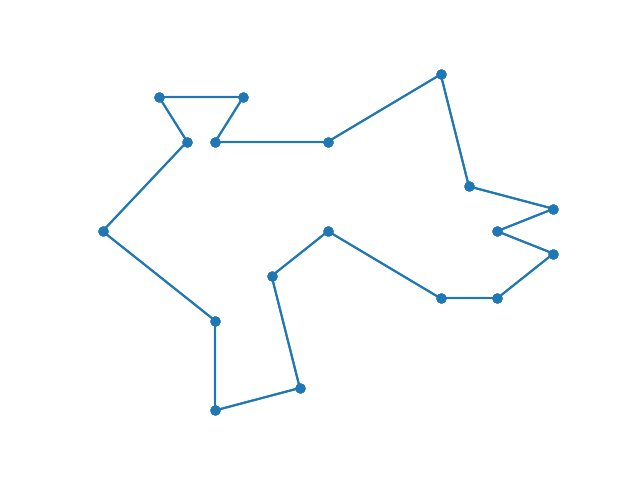
\includegraphics[width = 0.4\textwidth]{experiments/random.png}
    \caption{Arbitrarily shaped polygon.}
    \label{fig:random}
\end{figure}

\newpage
Figure \ref{fig:no_momentum} displays the area seen per iteration for the arbitrary polygon. Both the total and the individual areas seen by each guard are shown. Starting with almost the whole polygon seen, the guards are eventually optimally placed. Nonetheless, using momentum clearly makes a difference in Subfigure \ref{fig:no_momentum1}, than when not using it in Subfigure \ref{fig:no_momentum2}. Momentum allows the overall seen area to keep a steady trajectory towards its maximum. Additionally, guards quickly find their optimum in only 4 iterations, without many oscillations. In Subfigure \ref{fig:no_momentum2} however we  observe how the total area fluctuates. The guards display large jumps close to iterations 5 and 20. These jumps cause the overall progress towards the optimum to be less stable. For example, when guard 2 ($g2$) has a sudden drop in the area it sees around iteration 5, the total area seen naturally drops as well. The algorithm only recovers after iteration 20, when guard 0 ($g0$) makes another large jump. This behaviour also emphasises how the movement of one guard heavily influences the other guards' trajectories. As a result, the guards' trajectories to optimality become noisier and slower (more iterations are needed).
% Subfigure \ref{fig:no_momentum1} displays a more smoothened out trajectory for each guard. 


\begin{figure}[h!]
    \centering
    \begin{subfigure}{0.45\textwidth}
        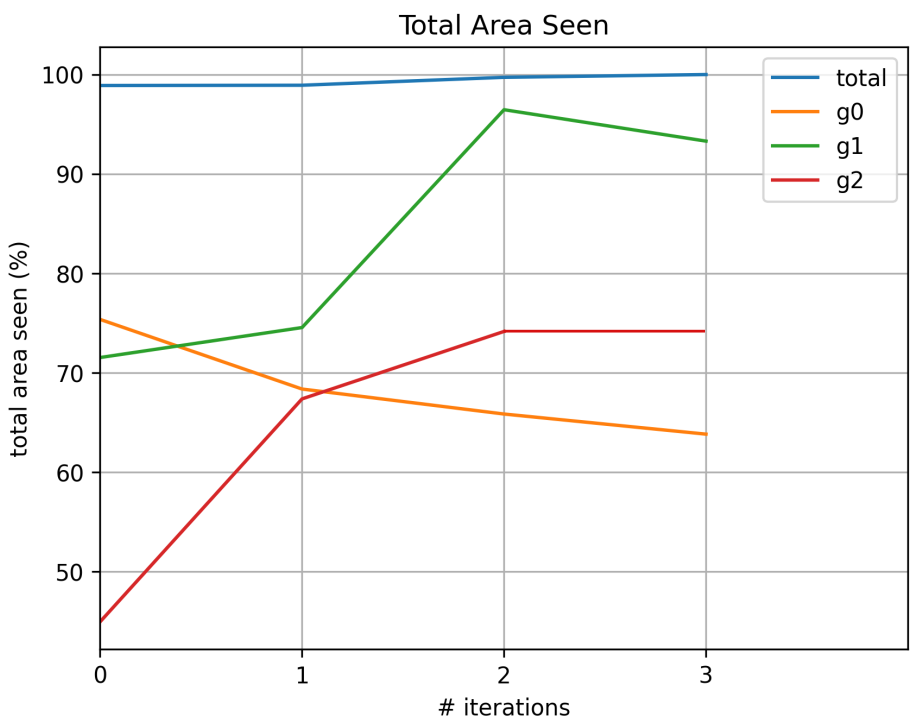
\includegraphics[width = \textwidth]{experiments/area_random_all2.png}
        \caption{All heuristics.}
        \label{fig:no_momentum1}
    \end{subfigure}
    \begin{subfigure}{0.45\textwidth}
        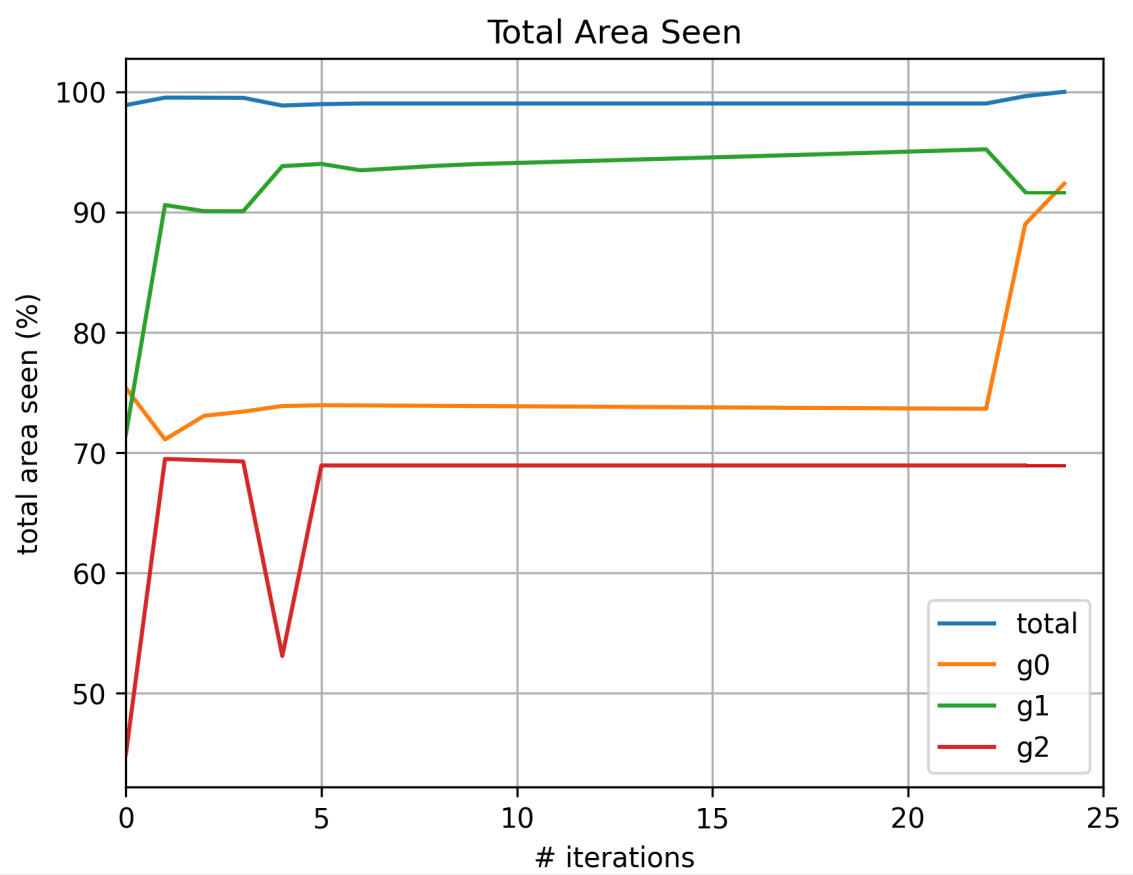
\includegraphics[width = \textwidth]{experiments/area_random_no_momentum2.png}
        \caption{No momentum.}
        \label{fig:no_momentum2}
    \end{subfigure}
    \caption{Total area seen per iteration for an arbitrary polygon guarded by 3 guards.}
    \label{fig:no_momentum}
\end{figure}

Thus, it becomes clearer how momentum allows the smoothening of noisy guard movements. We reckon that because guards are holding a steadier trajectory, they are more likely to achieve the optimum in less iterations. When not using momentum, the number of iterations increases substantially. Momentum appears to be a crucial improving heuristic to our whole algorithm, both in terms of speed-up and in the smoothness of the process.



\subsubsection{Without Pulling To and Onto the Reflex Vertex}
In this section we discuss the impact that the pull to and onto the reflex vertex heuristic has upon the behaviour of the algorithm. Sections \ref{sec:pull} and \ref{sec:pull_onto} introduced the pull to and onto reflex vertices heuristic, respectively. These heuristic tackles the idea that the closer a guard is to a reflex vertex, the stronger it is pulled towards it. If a guard is ``close enough'' to a reflex vertex, then the locally maximum seen area would be achieved by placing the guard on top of the reflex vertex. 
% We have defined ``close enough'' as a guard being closer than two thirds of the minimum distance between any two reflex vertices in the polygon.

Figure \ref{fig:no_pull_eg} displays the guards' movement both when we are using all the heuristics and when we are not pulling them onto reflex vertices. The polygon is arbitrarily shaped and requires three guards for full guarding. Subfigures \ref{fig:all_pull_pos0} and \ref{fig:all_pull_pos1} show how the green guard's movement changes when it is placed onto the reflex vertex. Subfigures \ref{fig:no_pull_pos0} and \ref{fig:no_pull_pos1} show how the guard's movement changes when it is pulled towards the reflex vertex, but not onto it. We  observe how in Subfigure \ref{fig:all_pull_pos1} the green guard is placed onto the reflex vertex. It then strives to reach the unseen polygon part in the upper left corner. On the other hand, in Subfigure \ref{fig:no_pull_pos1} the guard moves away from the reflex vertex.

\begin{figure}[h!]
    \centering
    \begin{subfigure}{0.45\textwidth}
        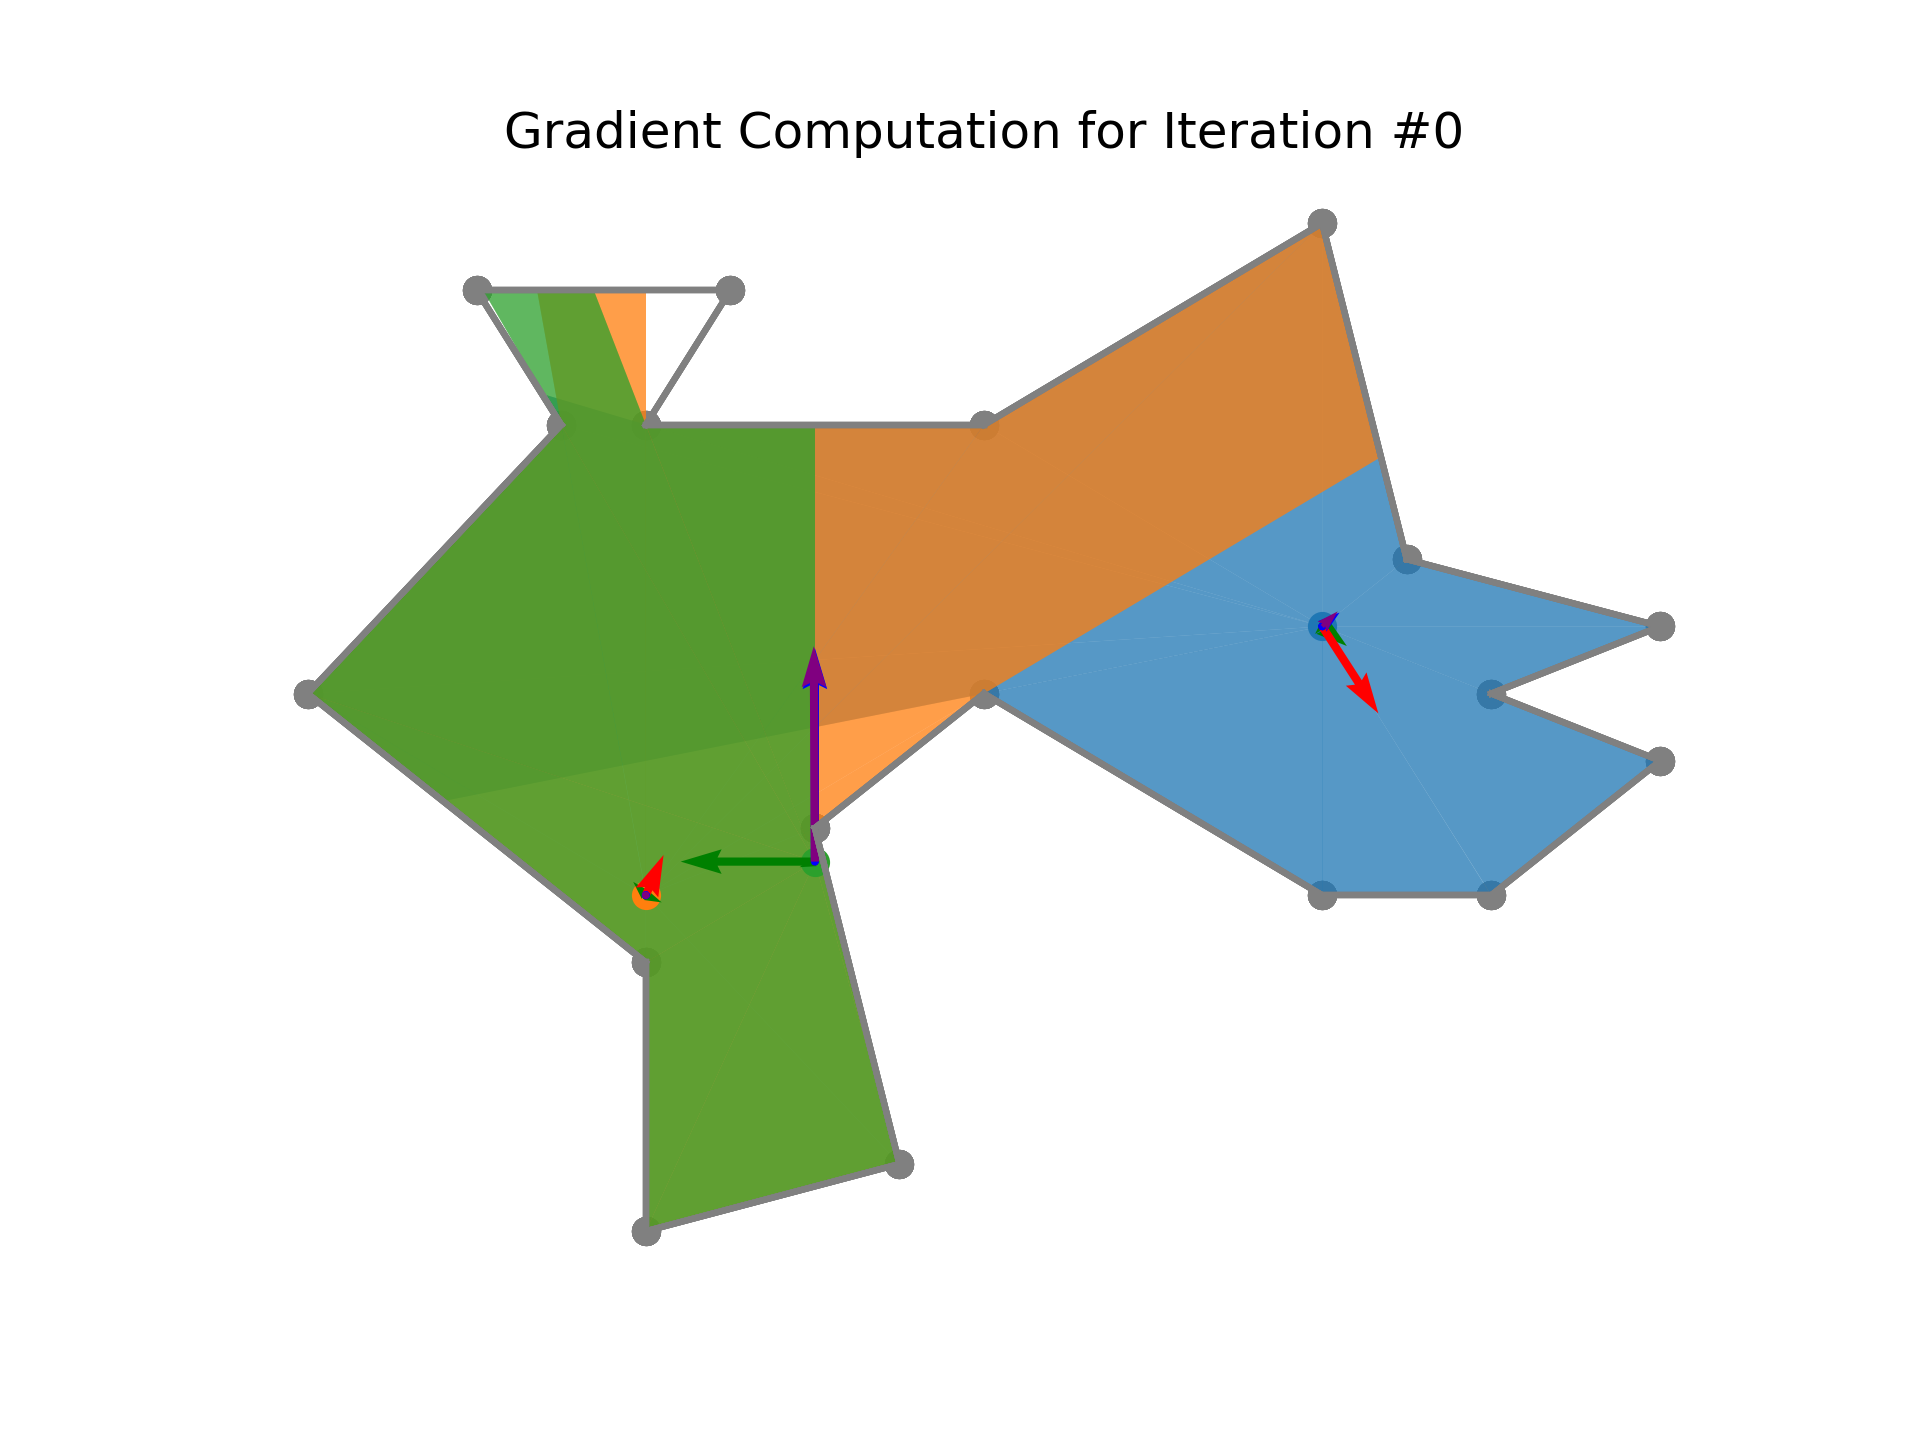
\includegraphics[width = \textwidth]{experiments/random_all_pull_pos0_fixed.png}
        \caption{All heuristics. The green guard is pulled towards the reflex vertex.}
        \label{fig:all_pull_pos0}
    \end{subfigure}
    \hfill
    % \vfill
    \begin{subfigure}{0.45\textwidth}
        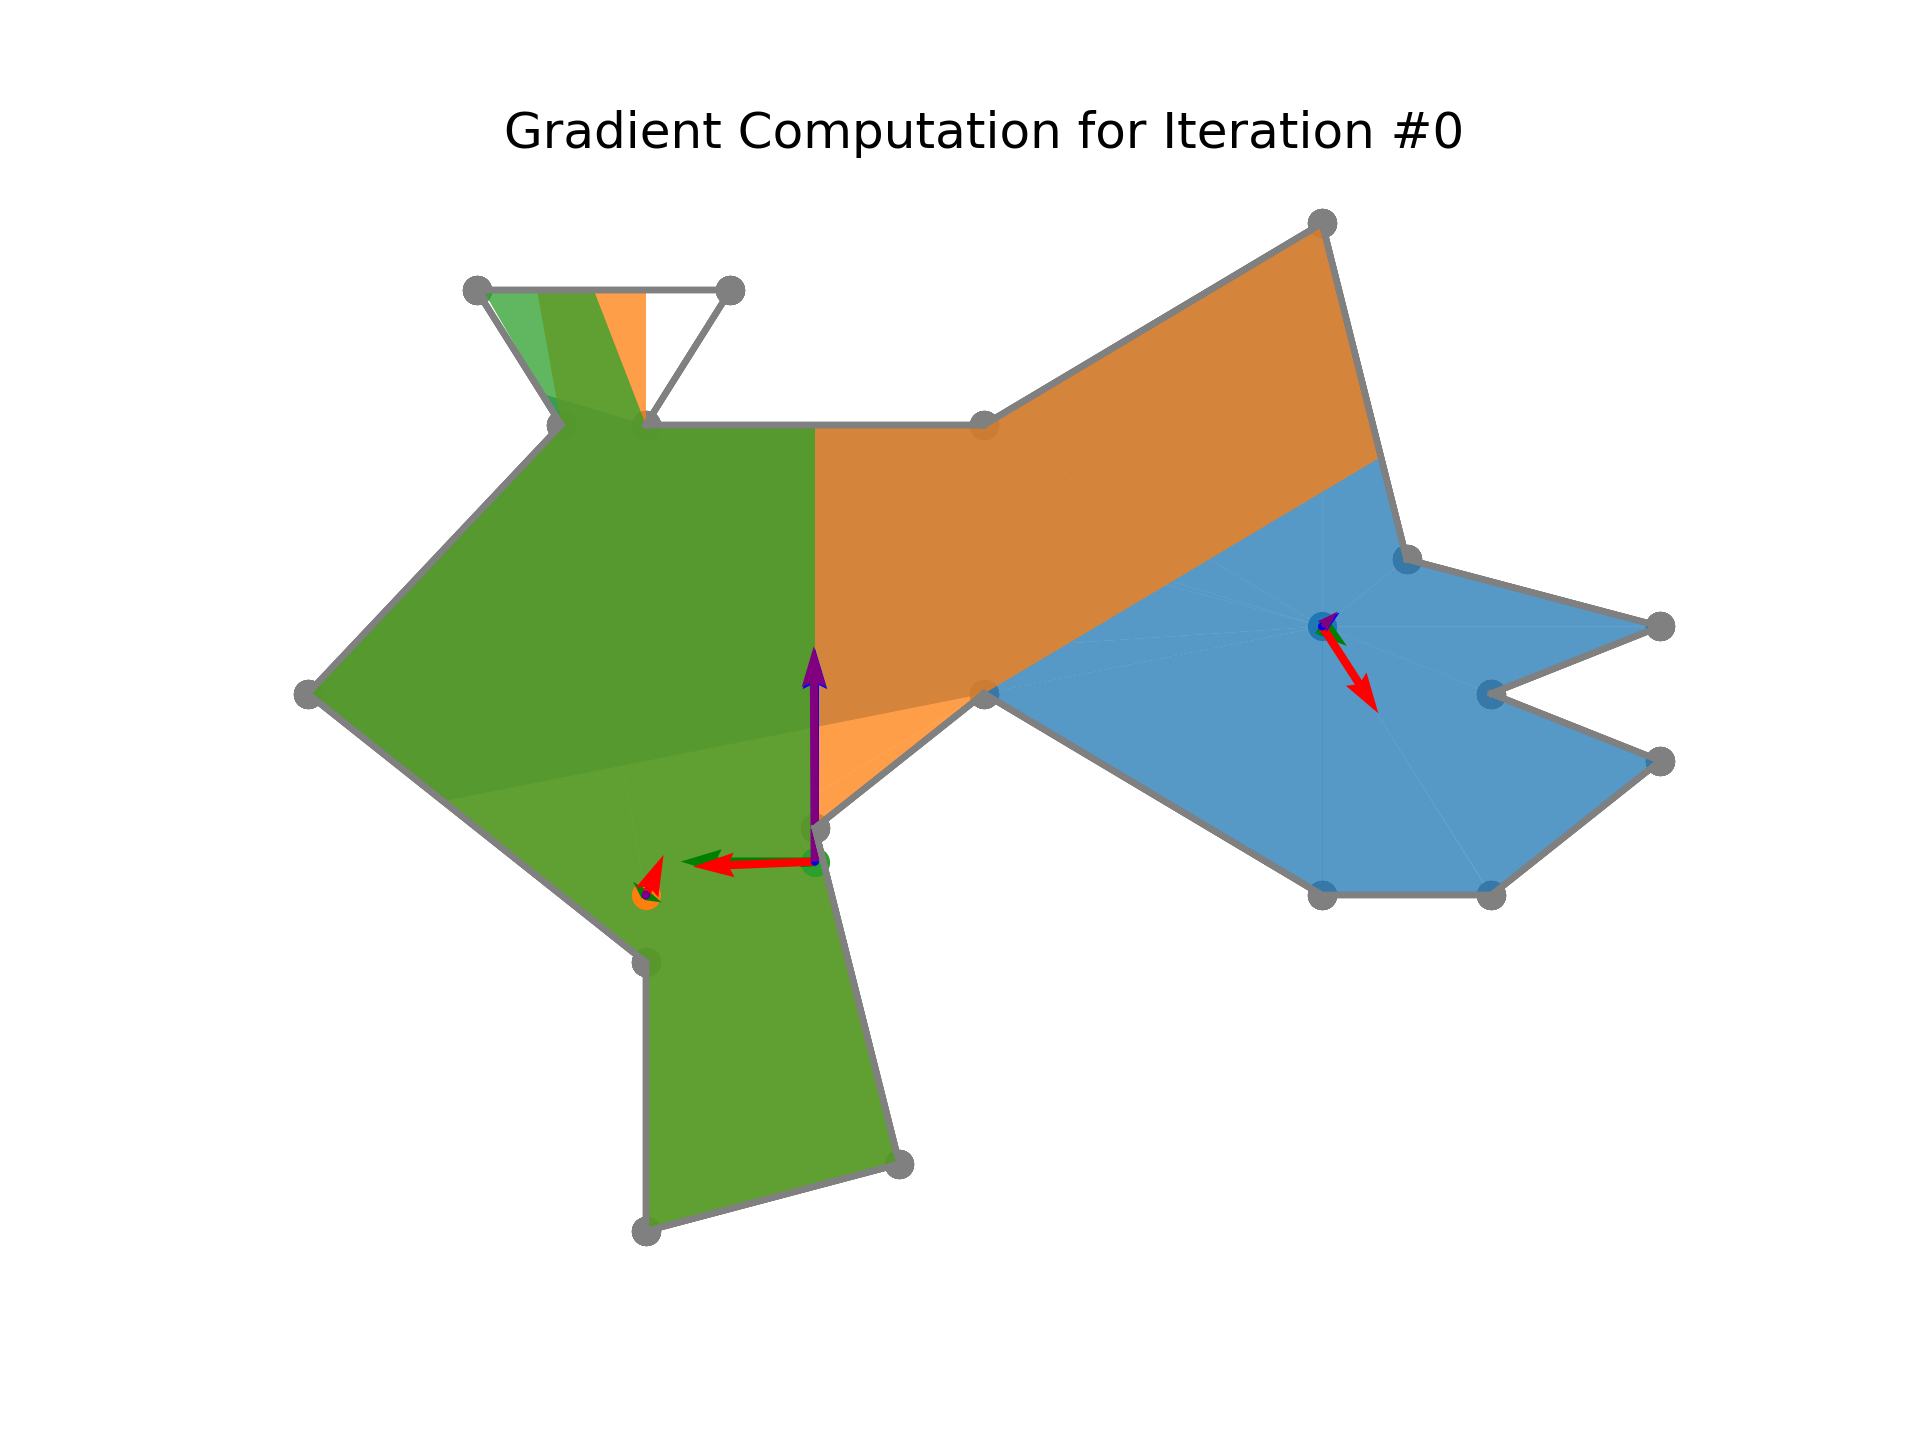
\includegraphics[width = \textwidth]{experiments/random_no_pull_pos0_fixed.png}
        \caption{No pull onto the reflex vertex. The green guard is pulled towards the reflex vertex.}
        \label{fig:no_pull_pos0}
    \end{subfigure}
    \begin{subfigure}{0.45\textwidth}
        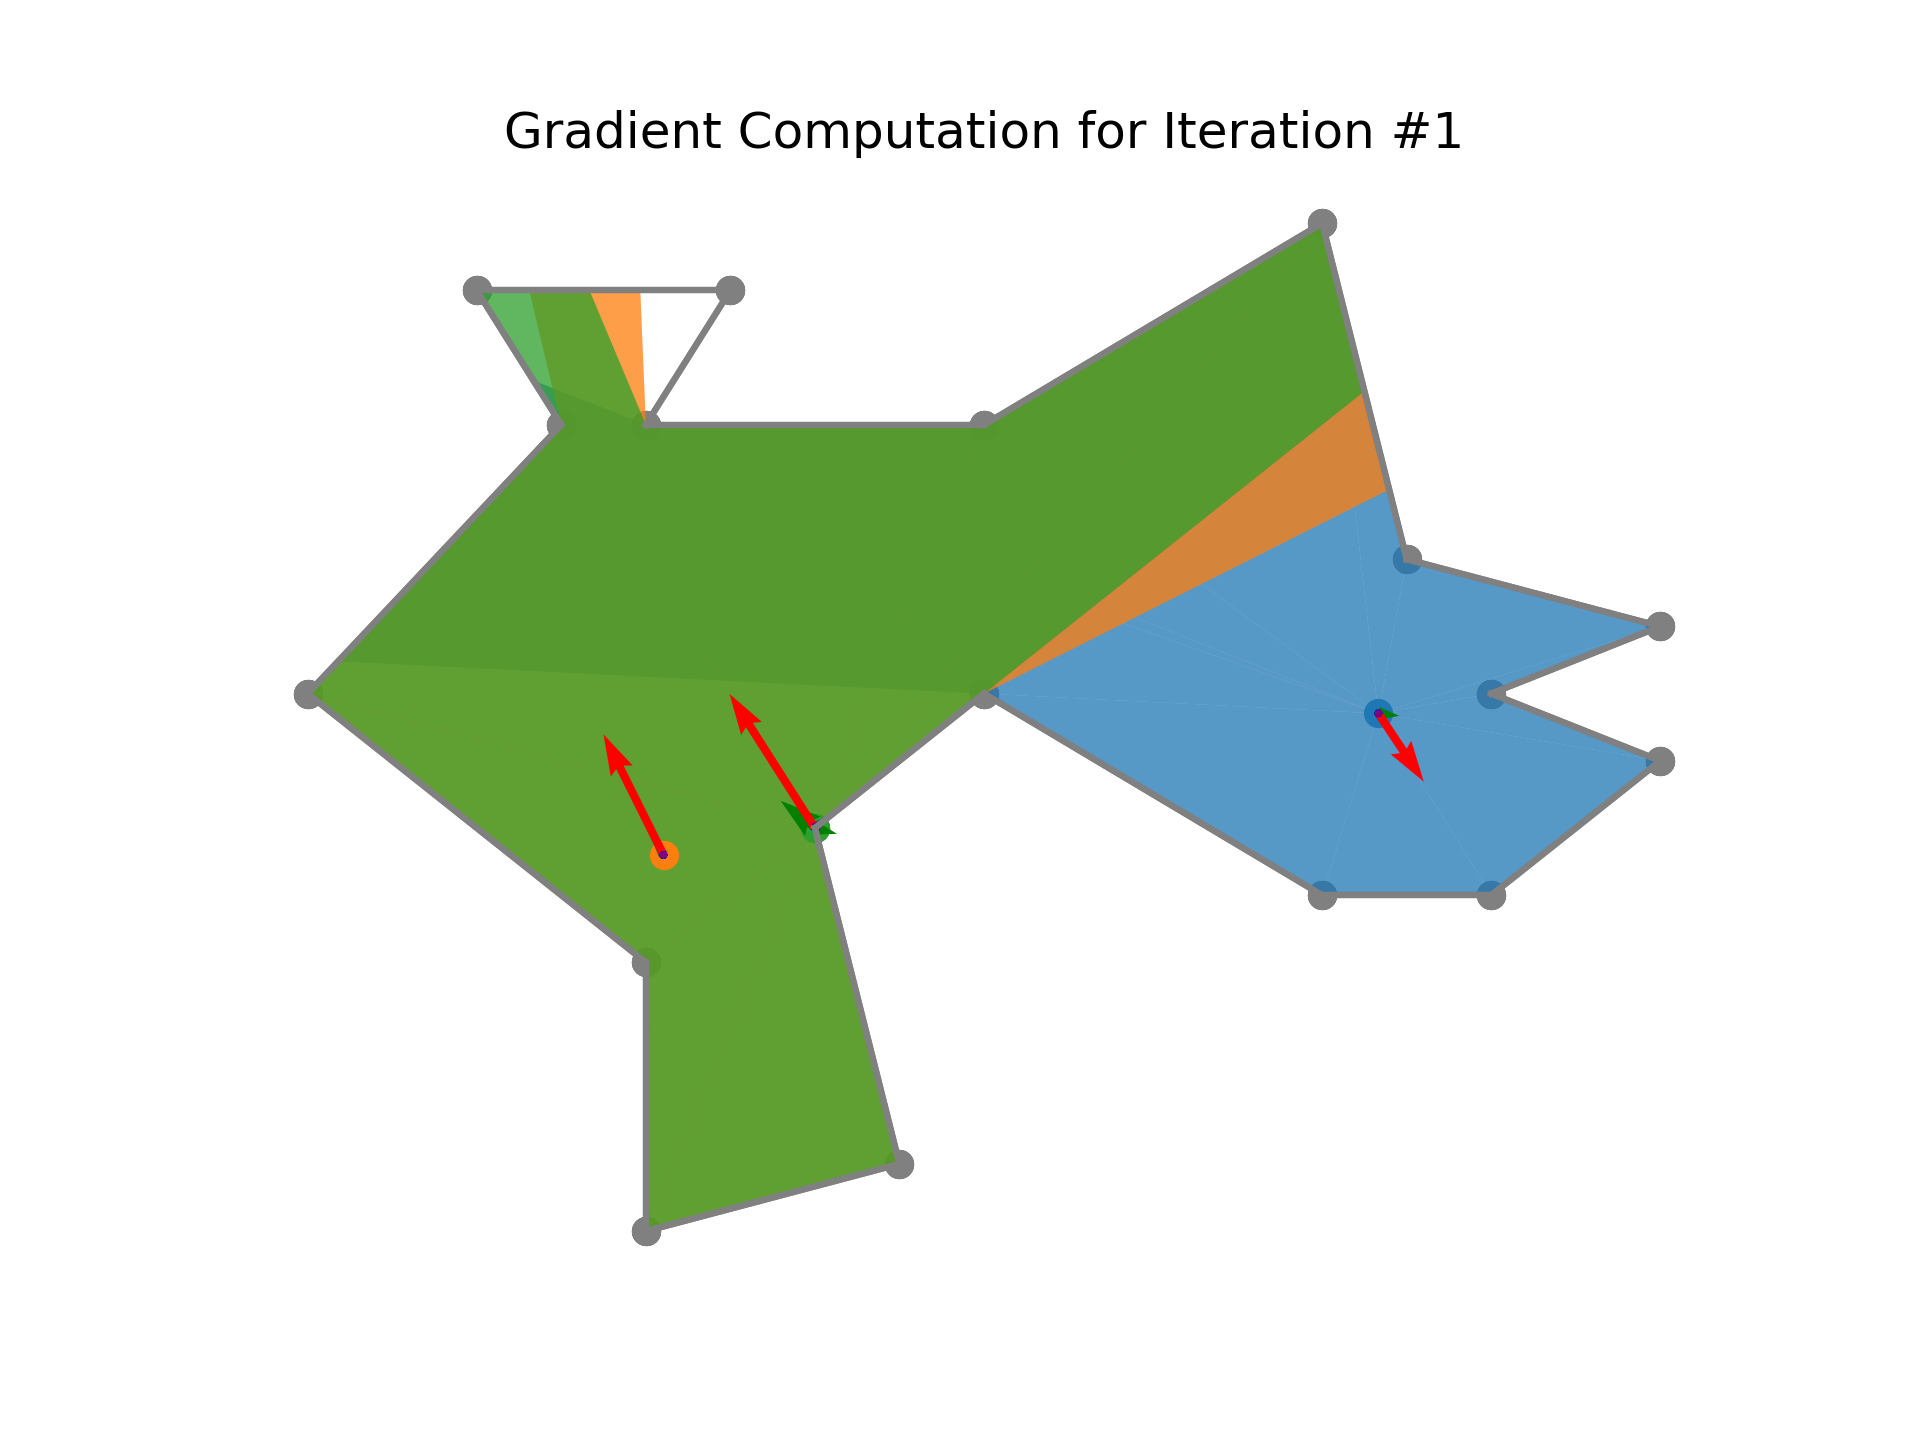
\includegraphics[width = \textwidth]{experiments/random_all_pull_pos1_fixed.png}
        \caption{All heuristics. The green guard is onto the reflex vertex.}
        \label{fig:all_pull_pos1}
    \end{subfigure}
    \hfill
    \begin{subfigure}{0.45\textwidth}
        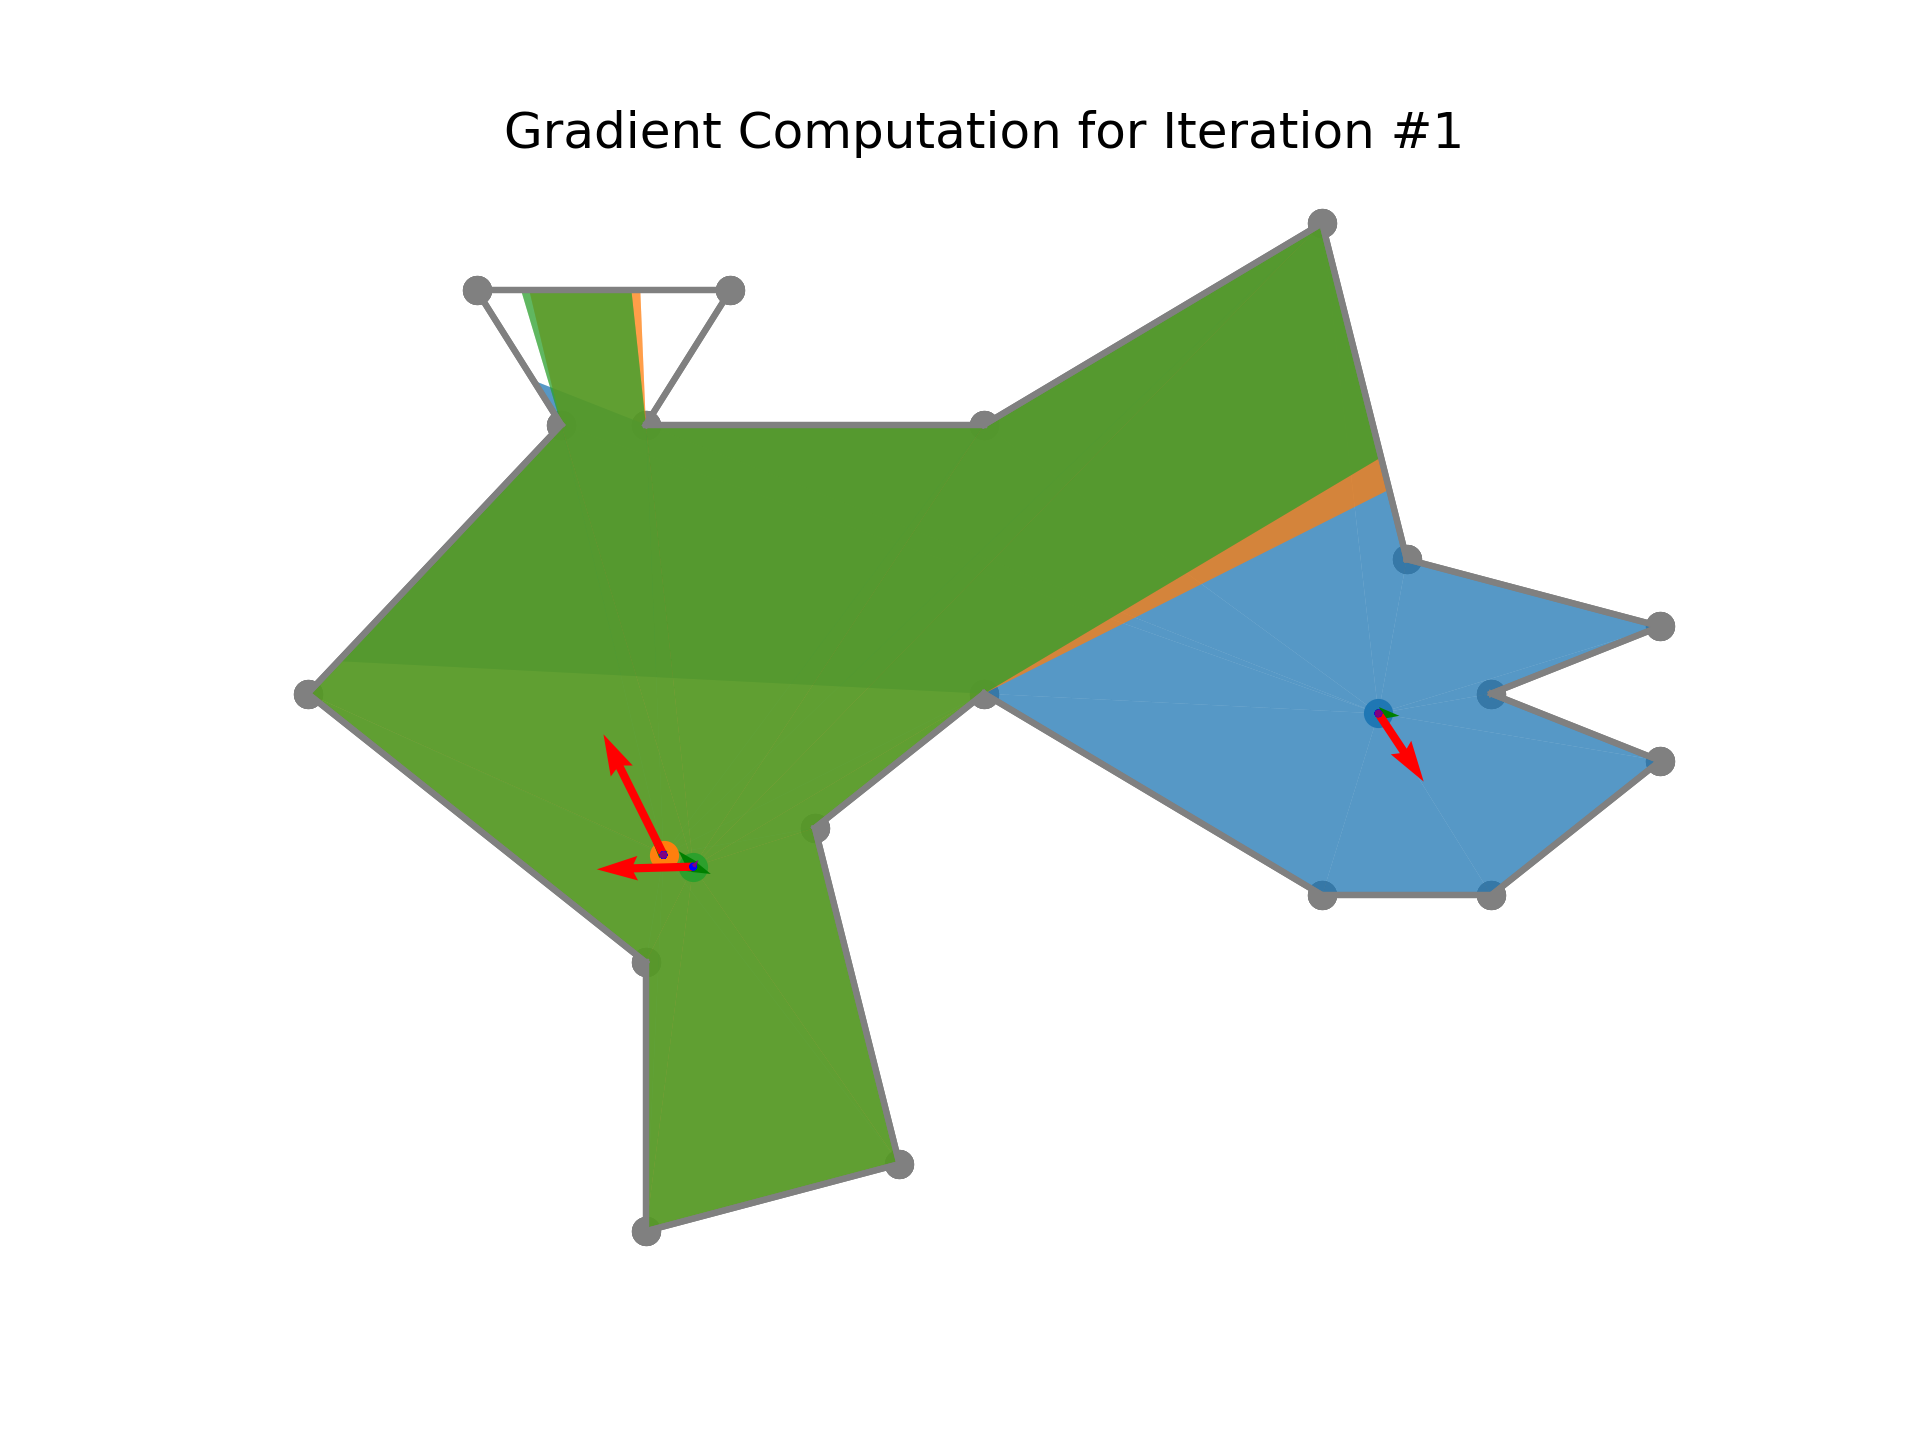
\includegraphics[width = \textwidth]{experiments/random_no_pull_pos1_fixed.png}
        \caption{No pull onto the reflex vertex. The green guard is placed according to the momentum computation.}
        \label{fig:no_pull_pos1}
    \end{subfigure}
    \caption{Example of different movements of guards with and without pulling them onto reflex vertices in an arbitrarily shaped polygon guarded by three guards.}
    \label{fig:no_pull_eg}
\end{figure}

\newpage
\paragraph{Evaluation and Results}
\label{evaluation}
We compare the performance of our algorithm in two settings: with all heuristics and without the pull to and onto reflex vertices. We observe this behaviour on the three polygons displayed in Figure \ref{fig:polygons}. For each polygon, the algorithm is run 20 times for each heuristic setting, each time with randomised guards coordinates. Our evaluation consists of comparing the average number of iterations required for the algorithm to finish. We additionally note the average iteration of the algorithm in the two cases.

\begin{figure}[h!]
    \centering
    \begin{subfigure}{0.3\textwidth}
        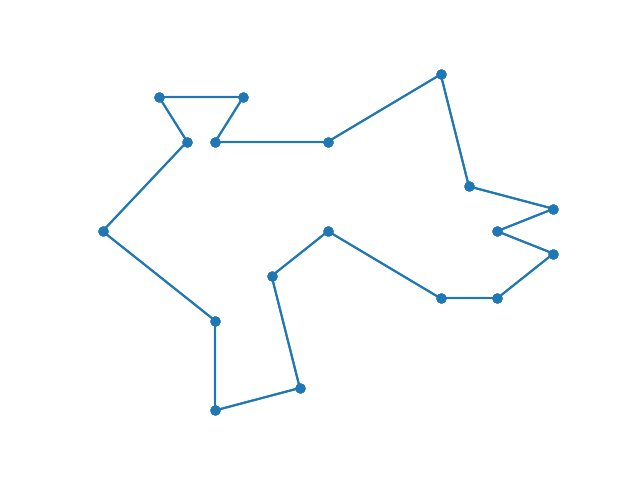
\includegraphics[width = \textwidth]{experiments/random.png}
        \caption{Arbitrarily shaped polygon that requires 3 guards for complete guarding (polygon 1).}
    \end{subfigure}
    \hfill
    \begin{subfigure}{0.3\textwidth}
        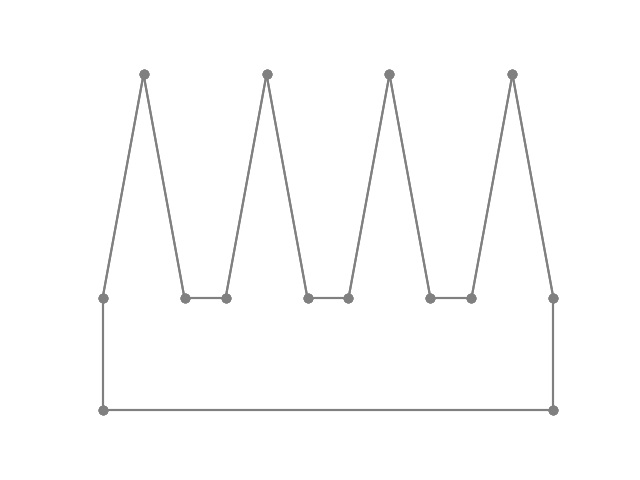
\includegraphics[width = \textwidth]{experiments/comb.png}
        \caption{Comb-shaped polygon with four teeth that requires 4 guards for complete guarding (polygon 2).}
    \end{subfigure}
    \hfill
    \begin{subfigure}{0.3\textwidth}
        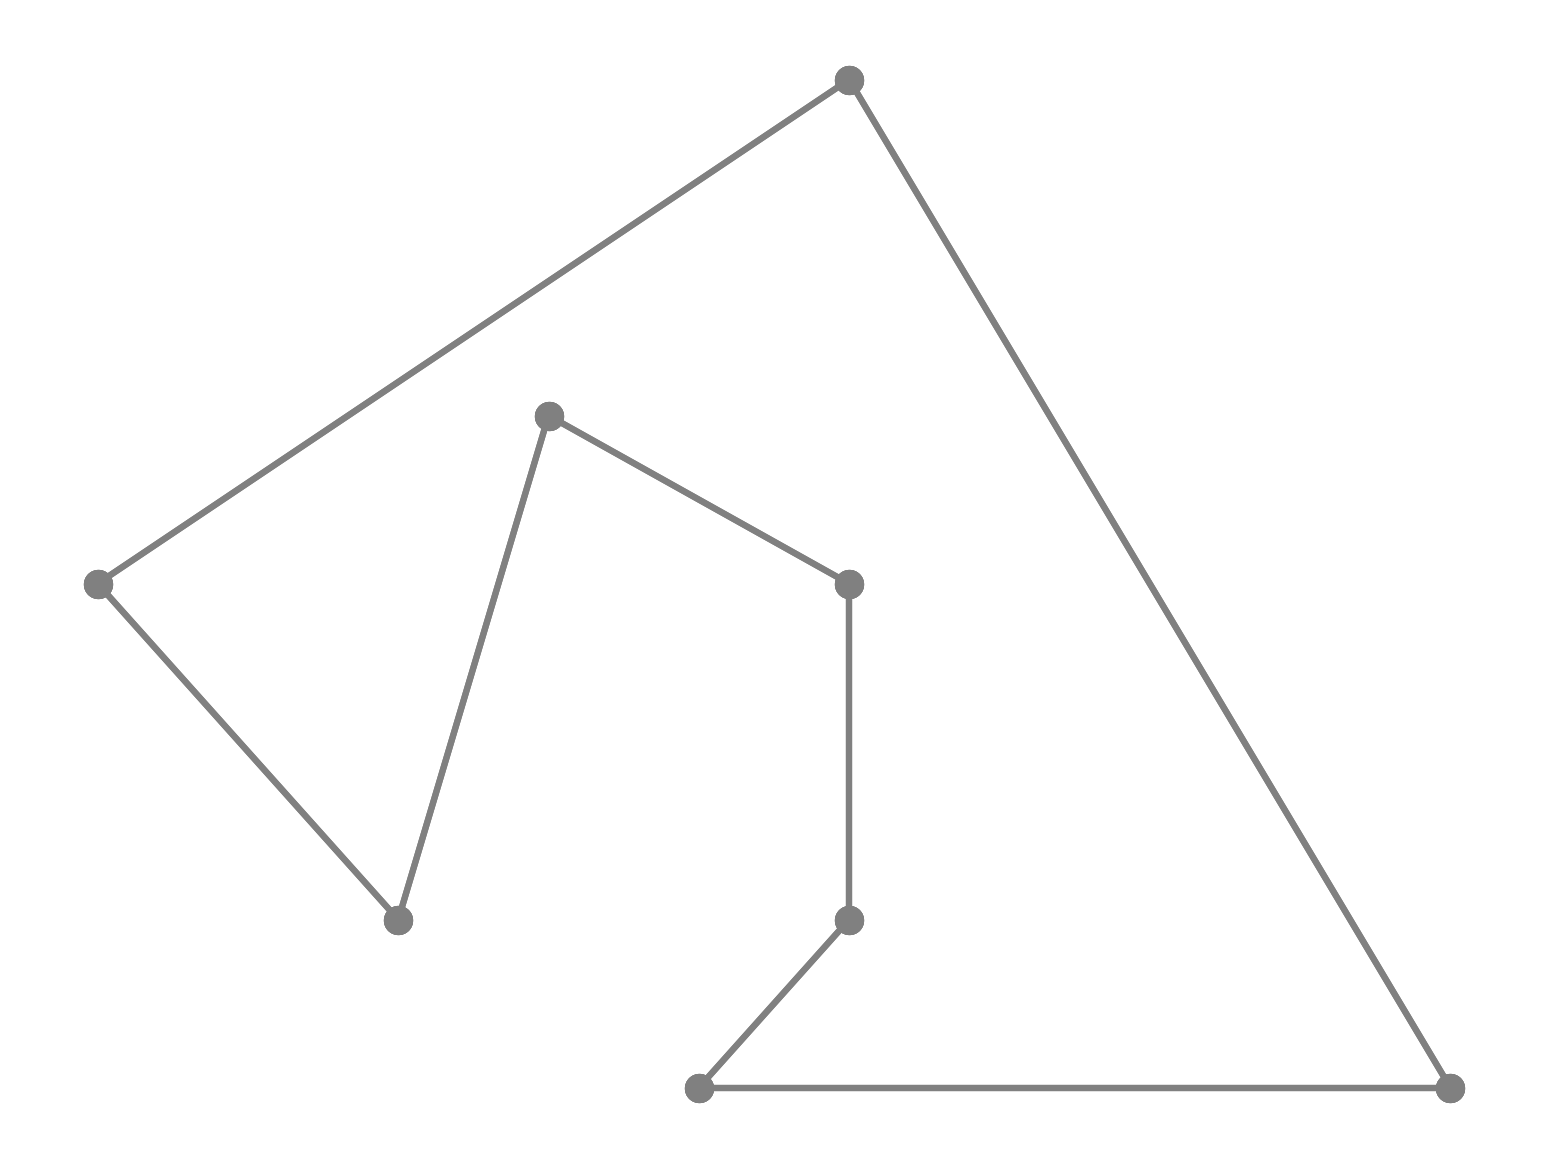
\includegraphics[width = \textwidth]{experiments/reflex_area.png}
        \caption{Arbitrarily shaped polygon that requires 2 guards for complete guarding (polygon 3).}
    \end{subfigure}
    \caption{The polygons used in our experiments.}
    \label{fig:polygons}
\end{figure}

Figure \ref{fig:avg_area} displays how the total area seen on average per iteration for the three polygons develops in the two cases. There is a quite clear distinction between using all heuristics and not using the pull for all the polygons. Overall, the algorithm requires more iterations when the pull heuristic is not used. 

The initial total area seen is higher on average for the all heuristics case than for the no pull case. Nonetheless, the algorithm in the no pull case compensates this disadvantaged start within the first 6 iterations for all polygons. In these first 6 iterations, both algorithms shoot towards the 100\% polygon visibility. When using all heuristics, the algorithm manages to achieve the full visibility in approximately just as many iterations as it took for the initial spike. In the case of the no pull algorithm, the convergence towards the optimum is much slower. 
Subfigure \ref{fig:avg_area_reflex_area} displays the worst such case (polygon 3), where the no pull algorithm took thrice as many iterations than in the all heuristics case. Subfigure \ref{fig:avg_area_comb} displays a less dramatic case for polygon 2. There not using the pull results in more smoothened out convergence curve, that is only a quarter longer than the all heuristics case. 
The difference in the average number of iterations happens due to the polygon shape. Polygons 1 and 3 are polygons where guards are required to travel past reflex vertices. So, the absence of the pull influences the speed and the efficiency of the movement much more. This is because without a pull, guards only travel around reflex vertices. Subfigure \ref{fig:avg_area_random} displays such a case for polygon 1. In the first 10 iterations without a pull, the guards appear to oscillate around reflex vertices. When using the pull, guards get stabilised closer to the reflex vertices. The reflex vertices in polygon 2 do not have such a strong influence. An optimal positioning in this case can also be achieved by moving around reflex vertices, and not necessarily towards them. 

\begin{figure}[h!]
    \centering
    \begin{subfigure}{0.45\textwidth}
        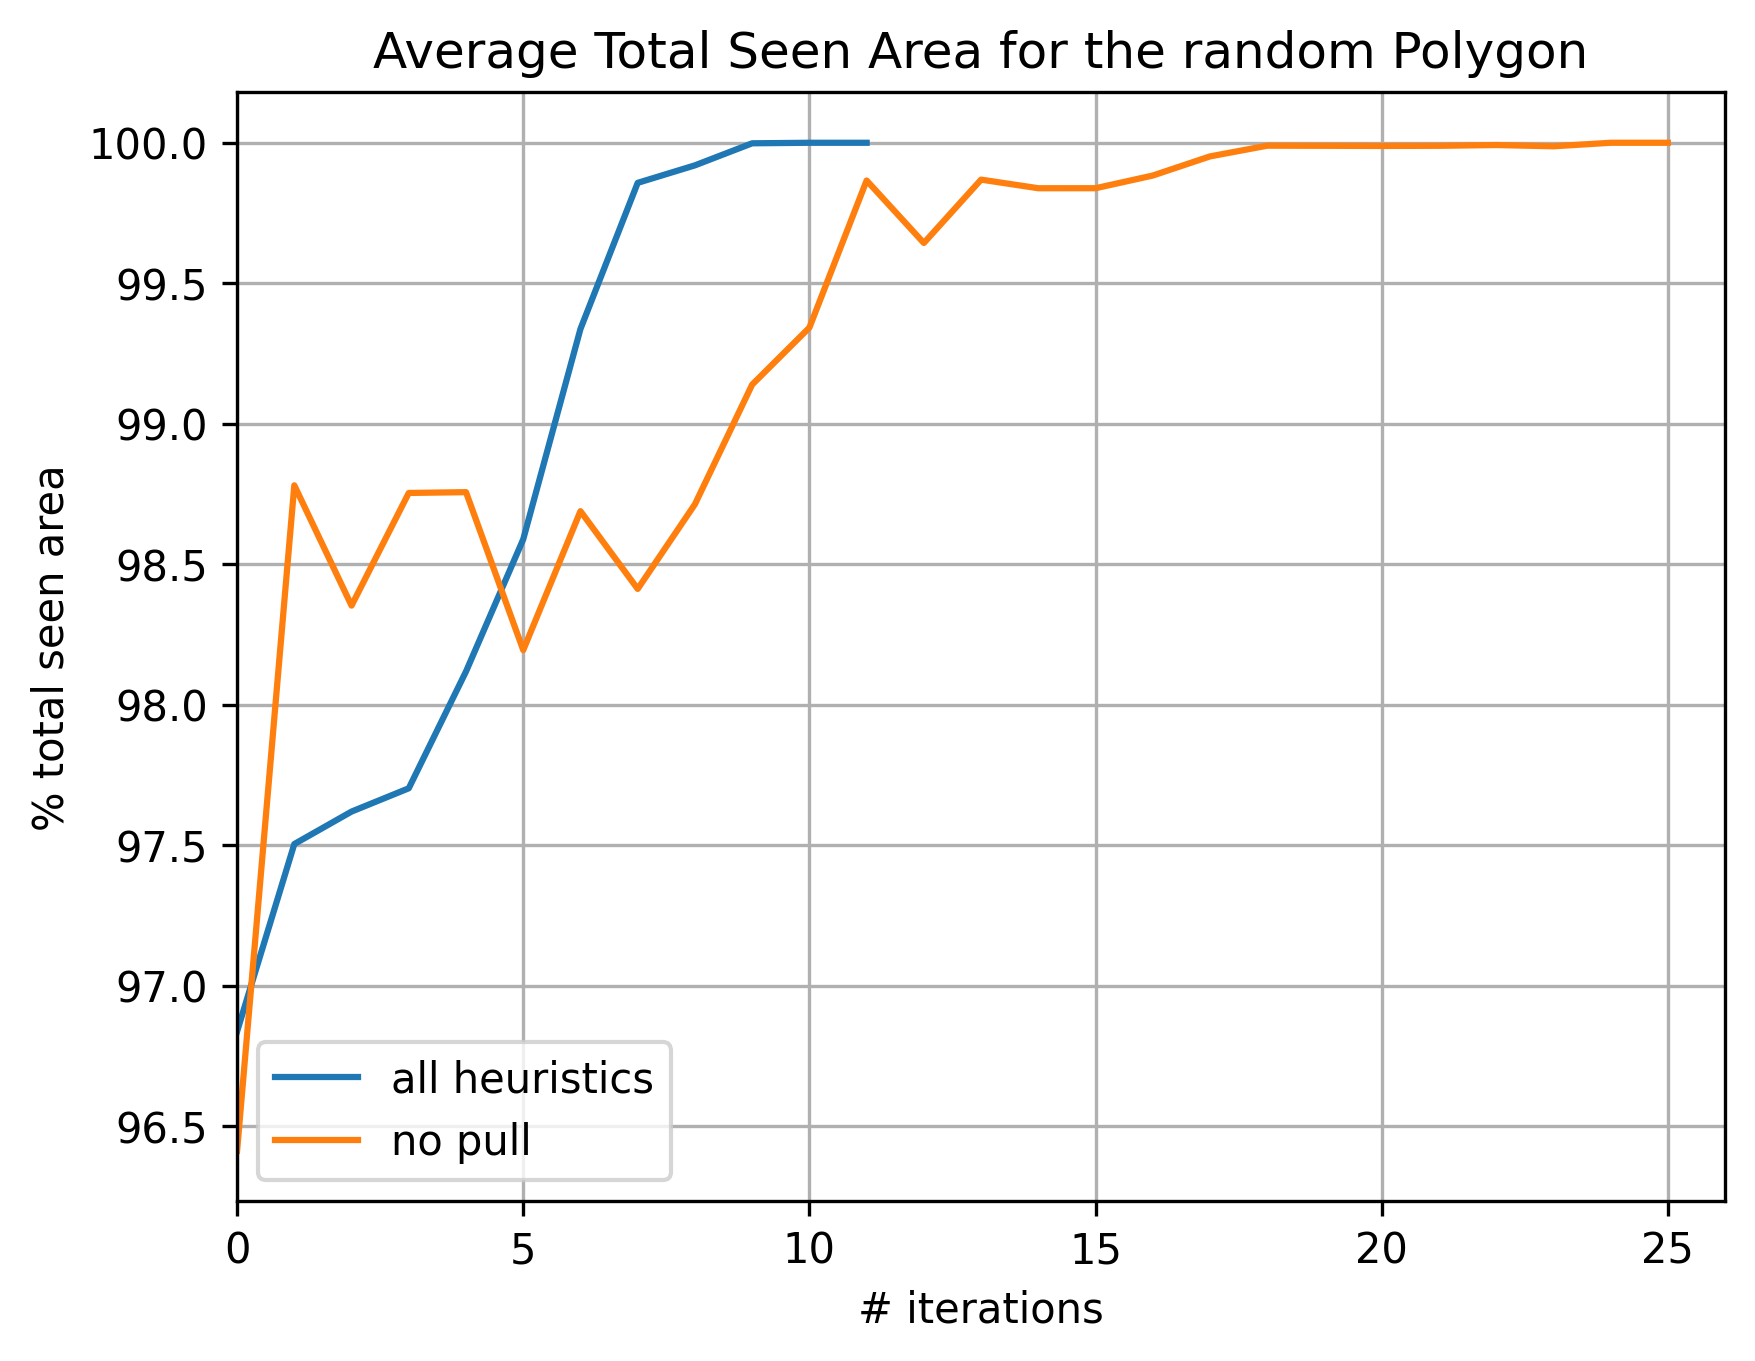
\includegraphics[width = \textwidth]{experiments/avg_area_random.png}
        \caption{Average total area seen per iteration for polygon 1.}
        \label{fig:avg_area_random}
    \end{subfigure}
    \hfill
    \begin{subfigure}{0.45\textwidth}
        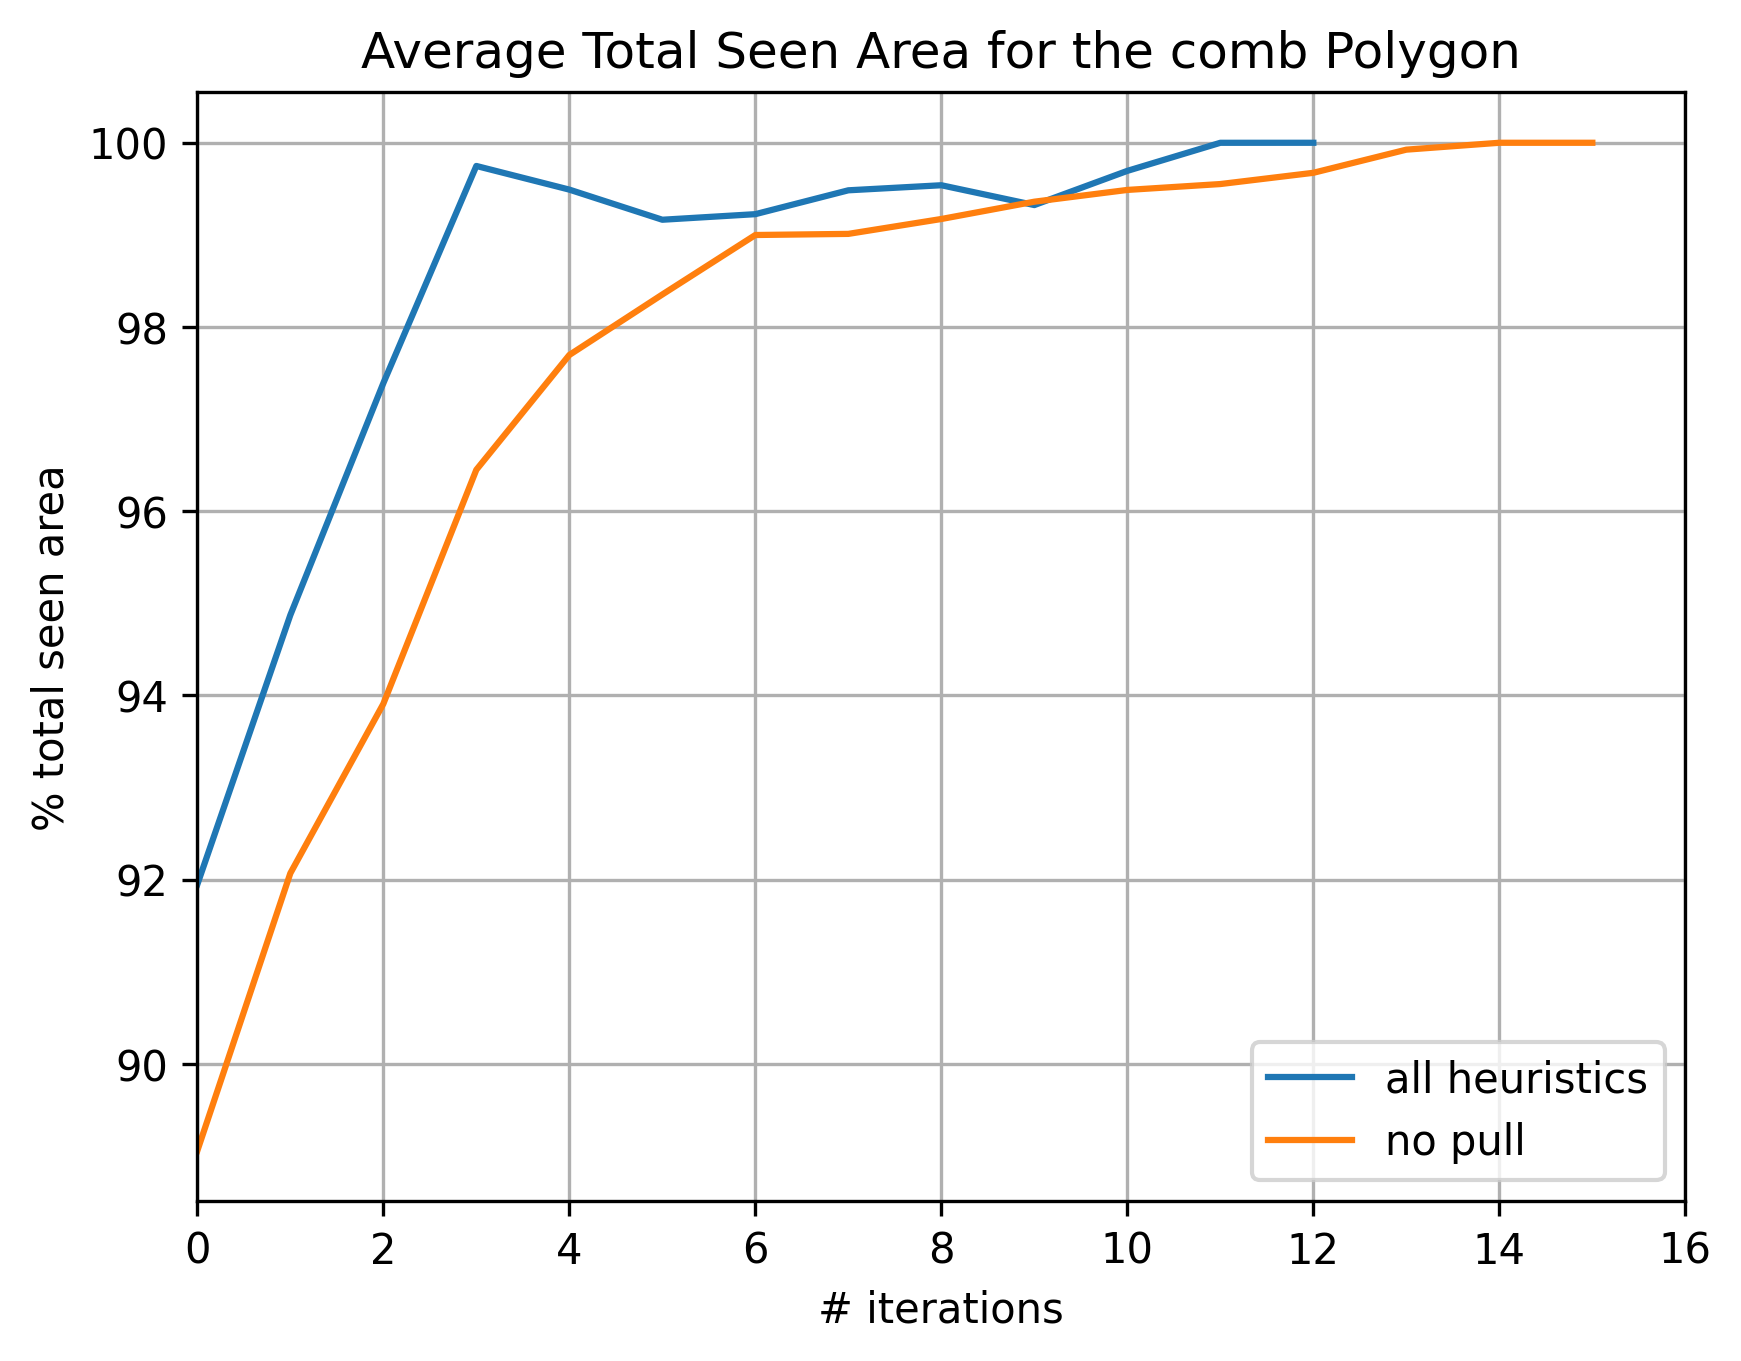
\includegraphics[width = \textwidth]{experiments/avg_area_comb.png}
        \caption{Average total area seen per iteration for polygon 2.}
        \label{fig:avg_area_comb}
    \end{subfigure}
    \begin{subfigure}{0.5\textwidth}
        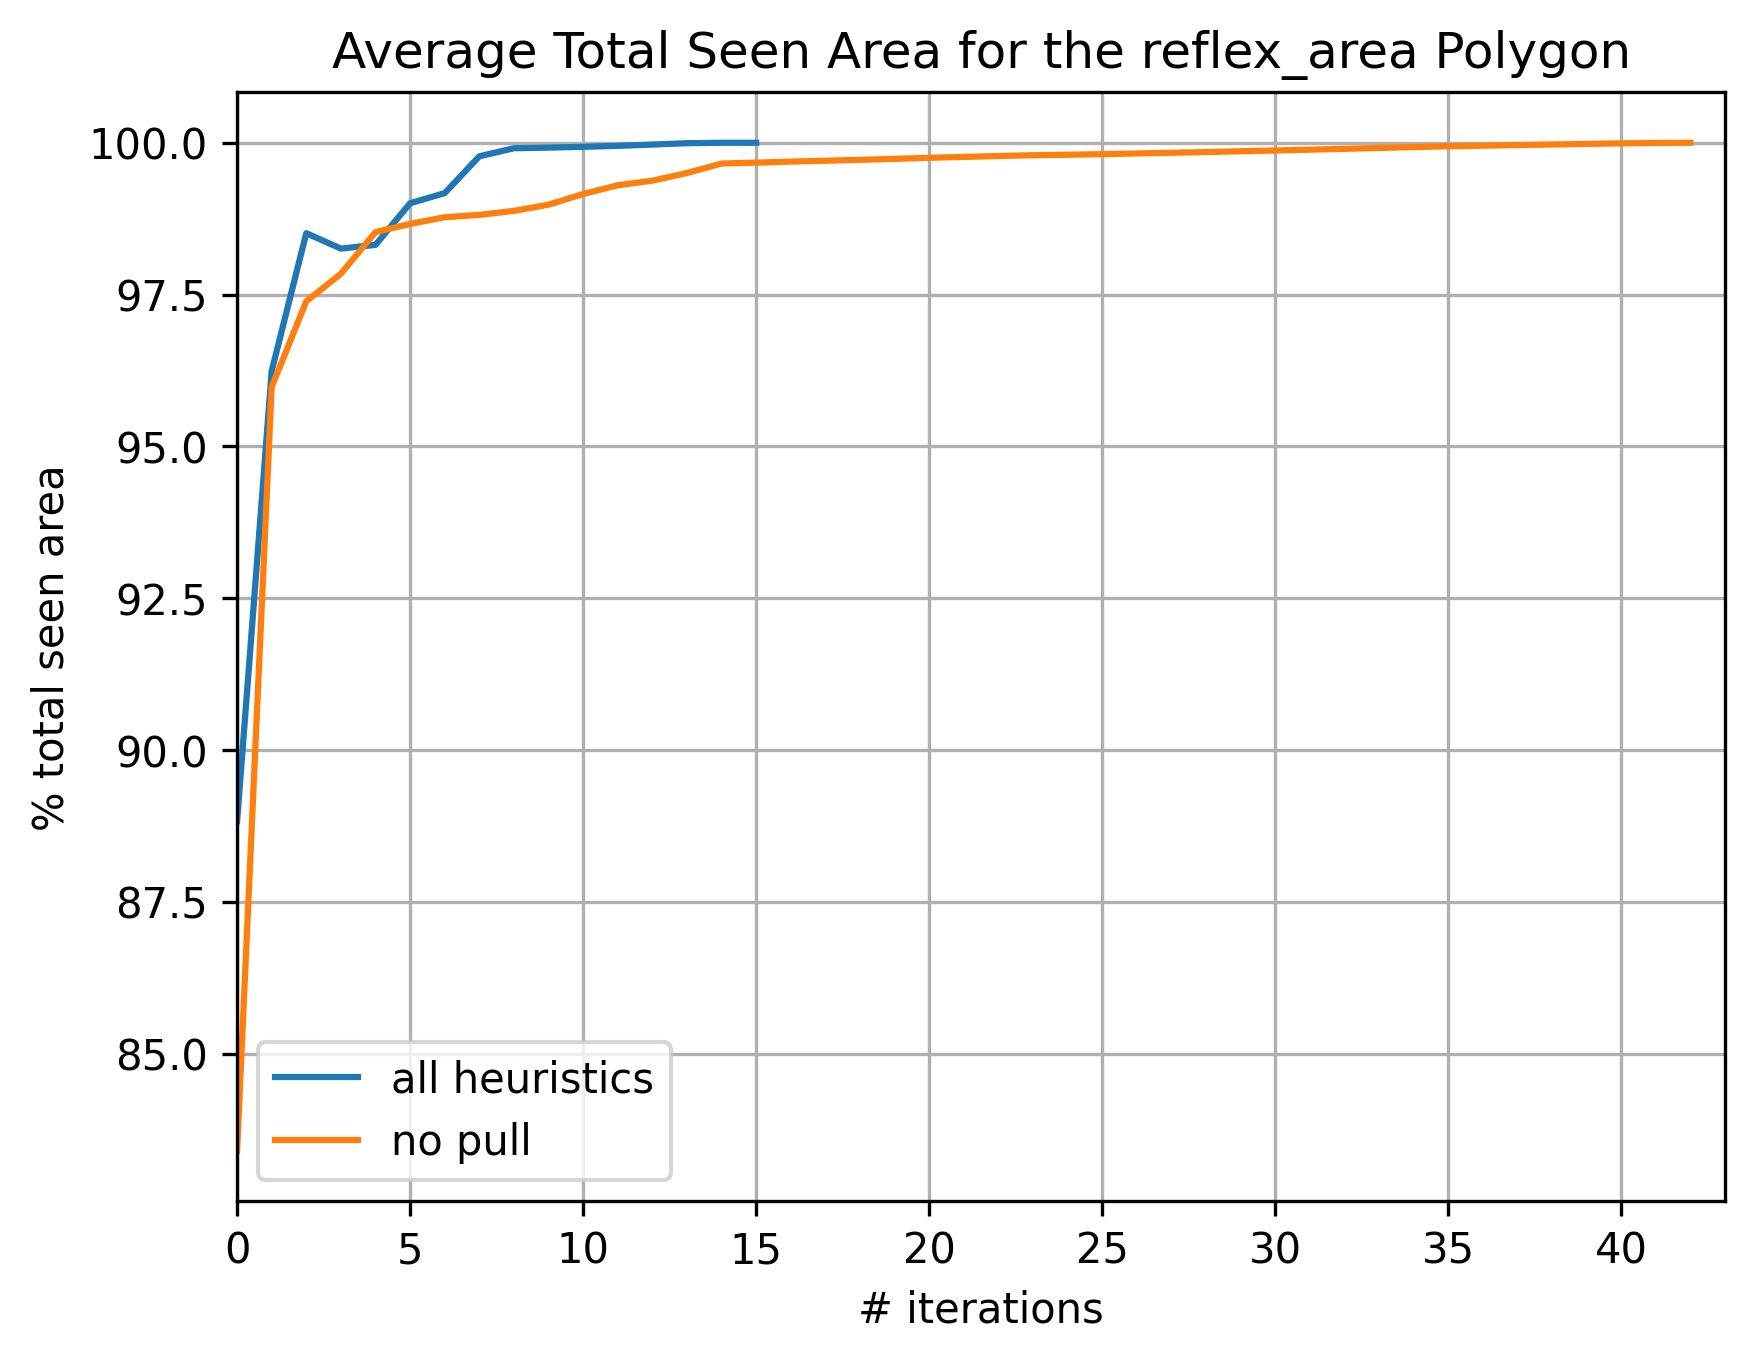
\includegraphics[width = \textwidth]{experiments/avg_area_reflex_area.png}
        \caption{Average total area seen per iteration for polygon 3.}
        \label{fig:avg_area_reflex_area}
    \end{subfigure}
    \caption{Average total area seen per iteration for all experimental polygons.}
    \label{fig:avg_area}
\end{figure}

\newpage
Figure \ref{fig:avg_iterations} displays the average number of iterations for all polygons in the two heuristic cases. As previously mentioned, it takes more iterations on average to solve a polygon when not using the pull heuristic. Nonetheless, not using this heuristic also results in a less predictable guard movement, with a higher standard deviation.

This is especially noticeable for polygons 1 and 3, in Subfigures \ref{fig:avg_iterations_random} and \ref{fig:avg_iterations_reflex_area}, respectively. In these two cases, it is unlikely that there is a statistical difference between the two approaches. This is because the median values of both cases lie within the first and third quantile of each other's boxes. However, the initial guard placement plays an important role in determining how well our algorithm performs. When no pull is used, some outliers appear. Those correspond to unfortunate initial guard coordinates. Using all heuristics mitigates this unlucky case, resulting in a more predictable guard movement that faster converge towards an optimum. A few outliers appear also when using all heuristics on polygon 3. They still perform better than the median performance when not using the pull heuristic. Nonetheless, the starting guard positioning in the case of all heuristics used on polygon 3 appears to be positively skewed. This means that on average the starting positioning of the guards gave the algorithm a head start.

In the case of polygon 2 in Subfigure \ref{fig:avg_iterations_comb}, the improved performance of the all heuristic algorithm becomes clearer. The median number of iterations lays underneath the first quantile when no pull is used. This indicates that a statistical difference between them could be likely. It is worth discussing what the implications of this difference are. We have discussed that the shape of polygon 2 allows guards to find an optimum solution similarly fast to when all heuristics are used. Still, the pull appears to play a statistically important role in the faster convergence towards the optimum. 

\begin{figure}[h!]
    \centering
    \begin{subfigure}{0.45\textwidth}
        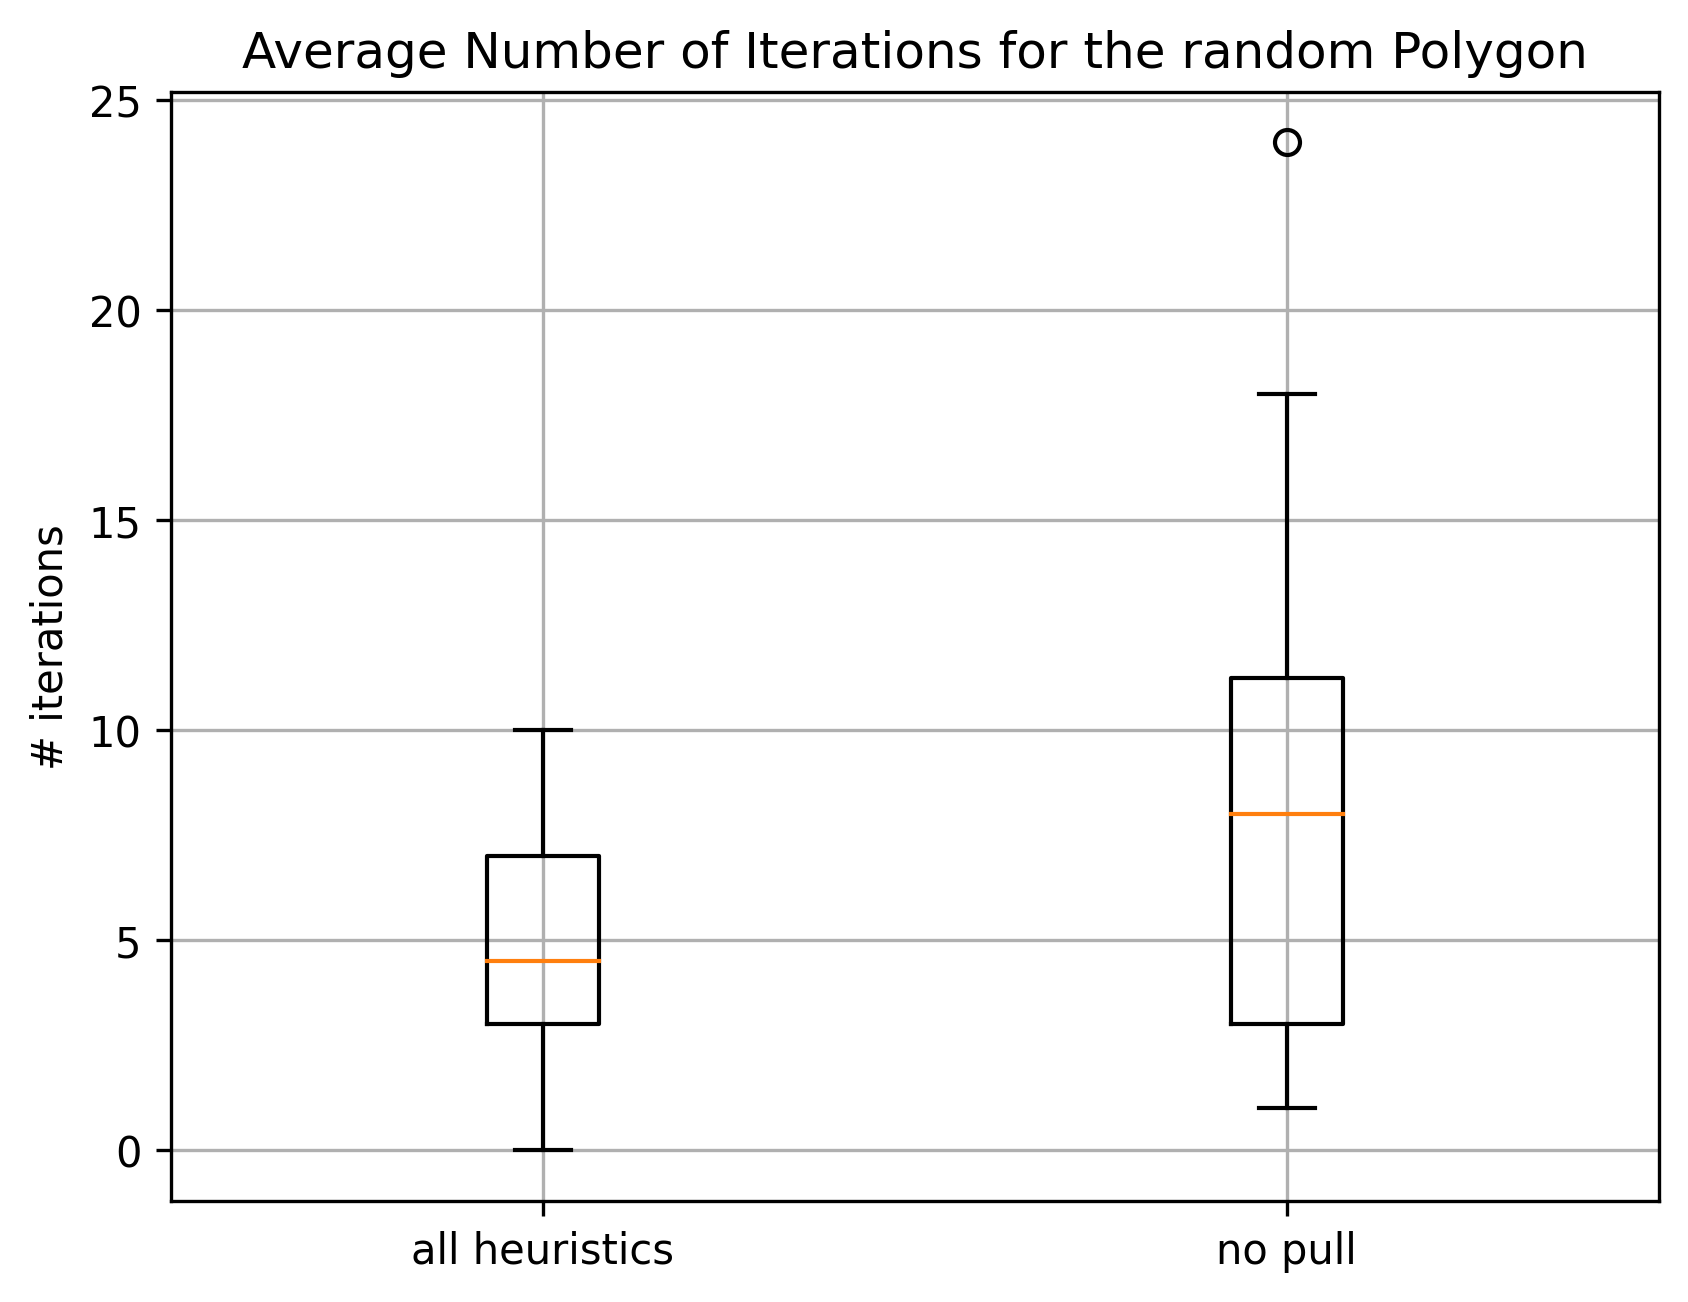
\includegraphics[width = \textwidth]{experiments/avg_iterations_random.png}
        \caption{Average number of iterations for polygon 1.}
        \label{fig:avg_iterations_random}
    \end{subfigure}
    \hfill
    \begin{subfigure}{0.45\textwidth}
        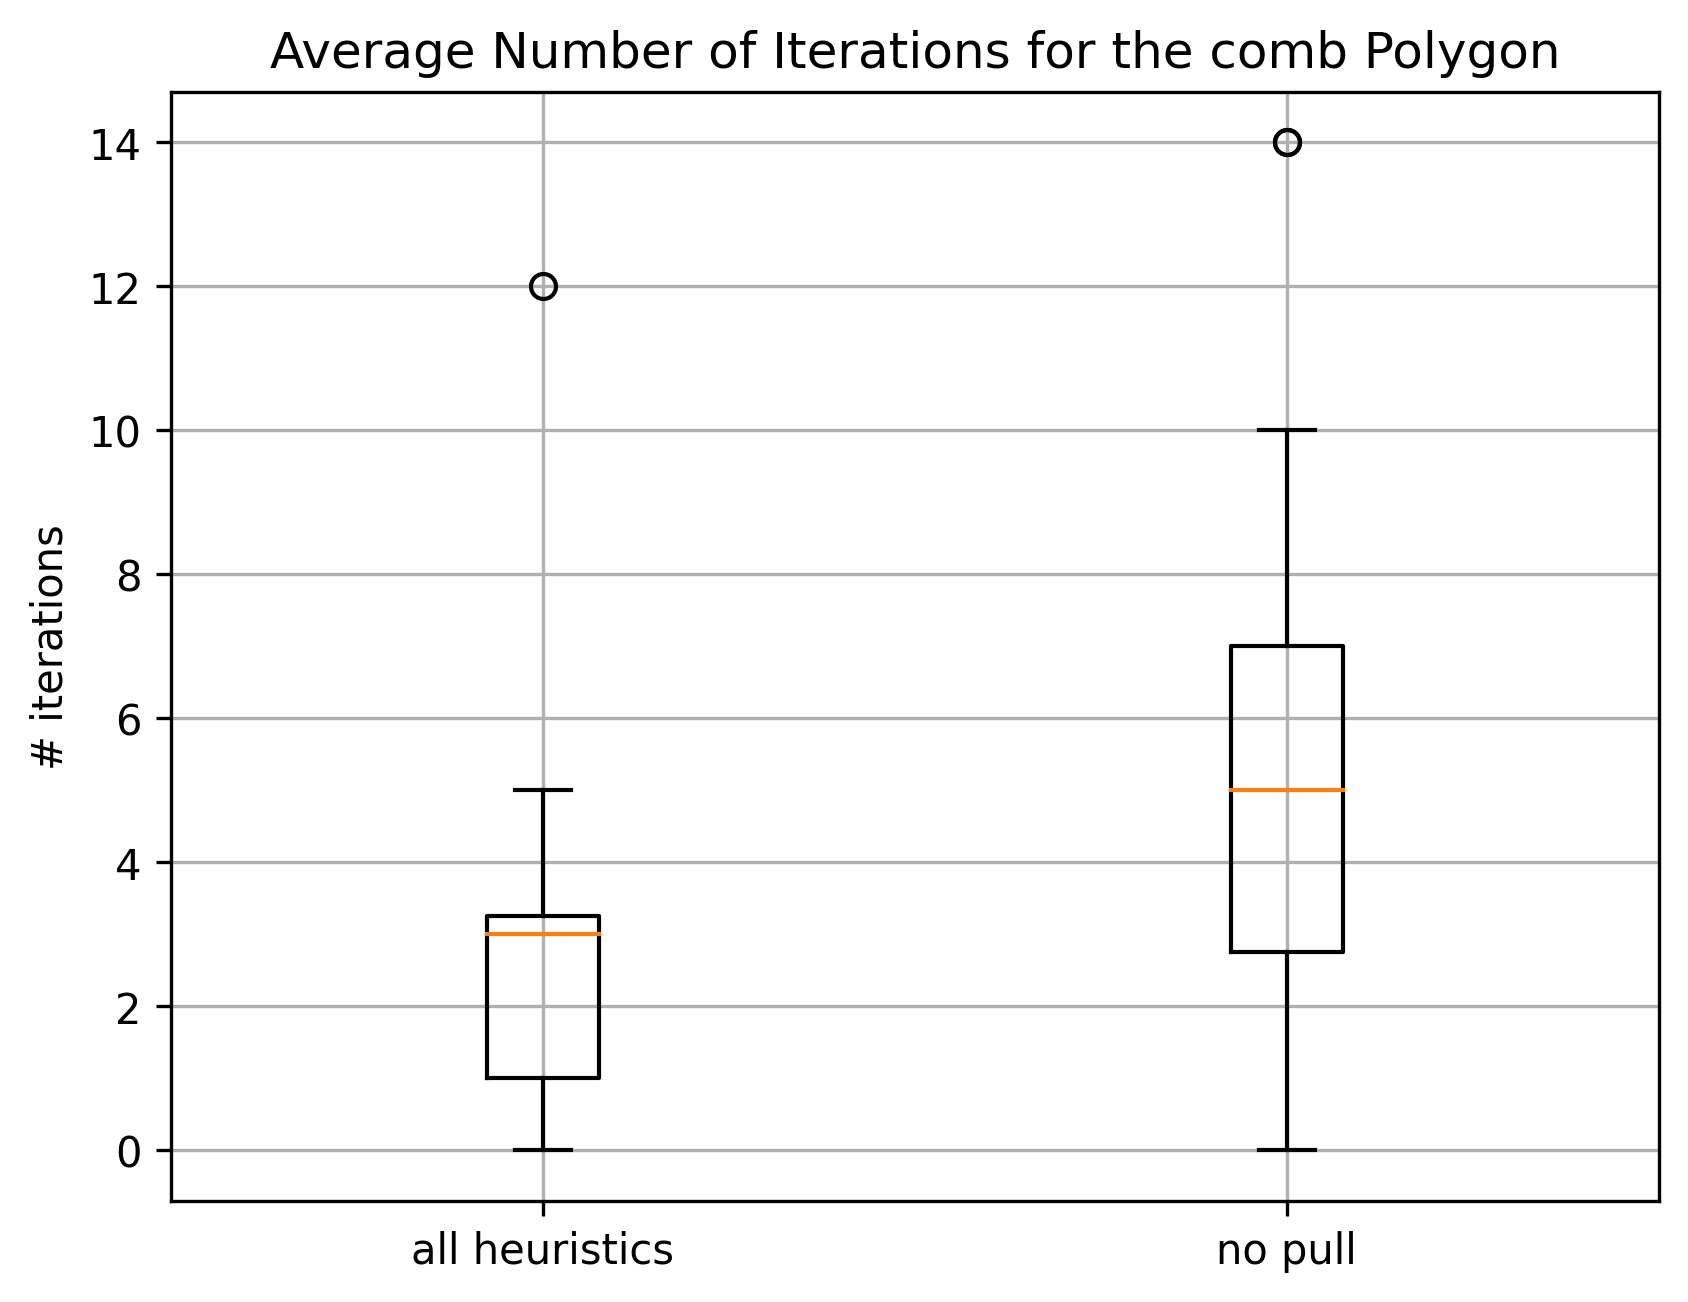
\includegraphics[width = \textwidth]{experiments/avg_iterations_comb.png}
        \caption{Average number of iterations for polygon 2.}
        \label{fig:avg_iterations_comb}
    \end{subfigure}
    \begin{subfigure}{0.5\textwidth}
        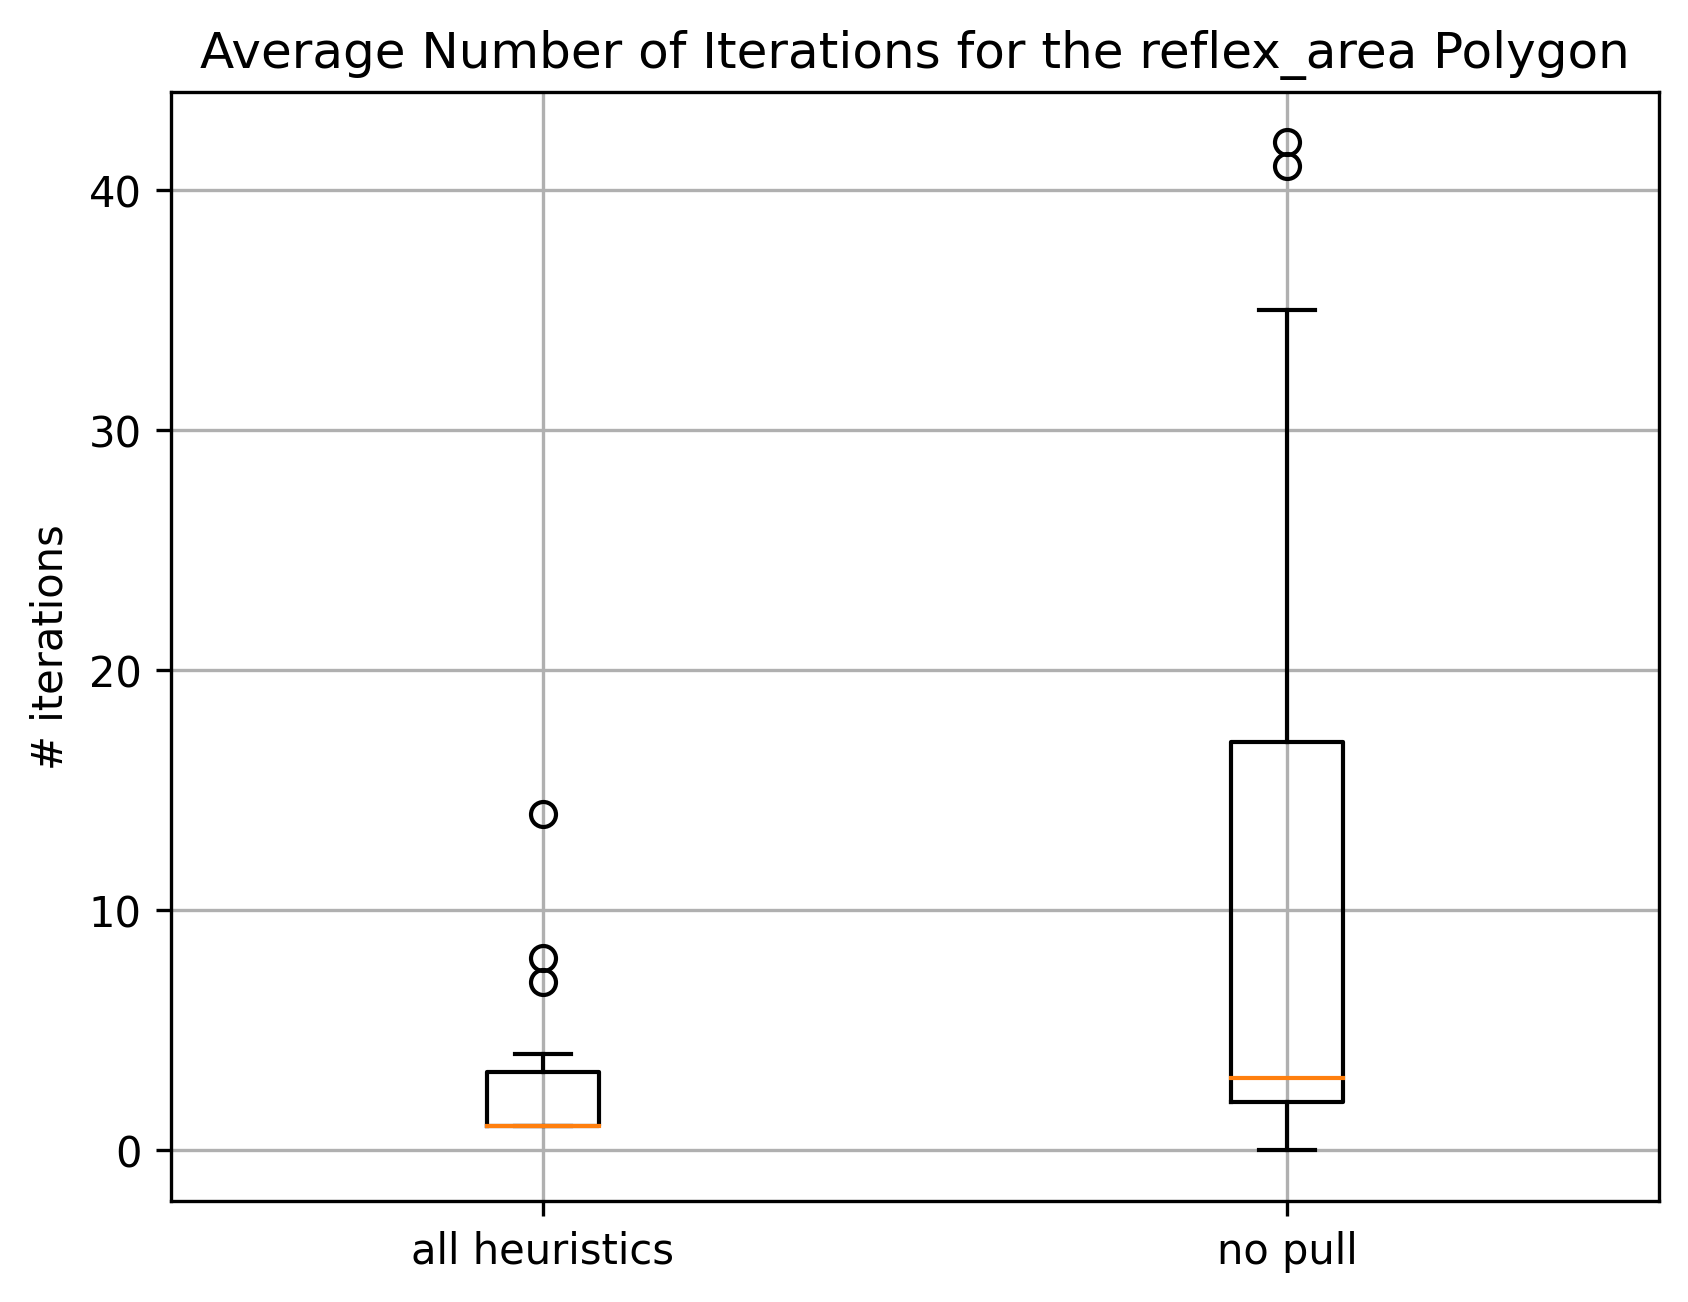
\includegraphics[width = \textwidth]{experiments/avg_iterations_reflex_area.png}
        \caption{Average number of iterations for polygon 3.}
        \label{fig:avg_iterations_reflex_area}
    \end{subfigure}
    \caption{Average number of iterations for all experimental polygons.}
    \label{fig:avg_iterations}
\end{figure}

% These events are also observed in the two area plots in Figure \ref{fig:no_pull_plots}. The case when the green guard is not placed on top of the reflex vertex results in more iterations (Subfigure \ref{fig:area_no_pull}). This is due to the fact that the green guard cannot maximise its locally seen area by being placed on the reflex vertex. So, it needs to move around more before finding its optimal path. This is also displayed in how the total area seen lowers and then rises in between iterations 1 and 4. Note that that the red guard does not move in iteration 4 because the other two guards have already covered the whole polygon. Conversely, Subfigure \ref{fig:area_all_pull} displays how the green guard quickly moves towards the last part of the polygon that was not yet seen. This results in a steady increase in the total seen area.

Therefore, we believe that pulling guards towards reflex vertices results in reaching the optimum in less iterations. This appears to be an improvement for all polygon shapes, regardless of whether guards need to move only around or also towards reflex vertices. This difference is less likely to be supported statistically for polygons with stronger pulls towards reflex vertices. Nonetheless, on average, the algorithm can solve polygons up to three times as fast when using all heuristics than when not using the pull.

% \newpage

% \vfill
% \begin{figure}[!h]
%     \begin{subfigure}{0.45\textwidth}
%         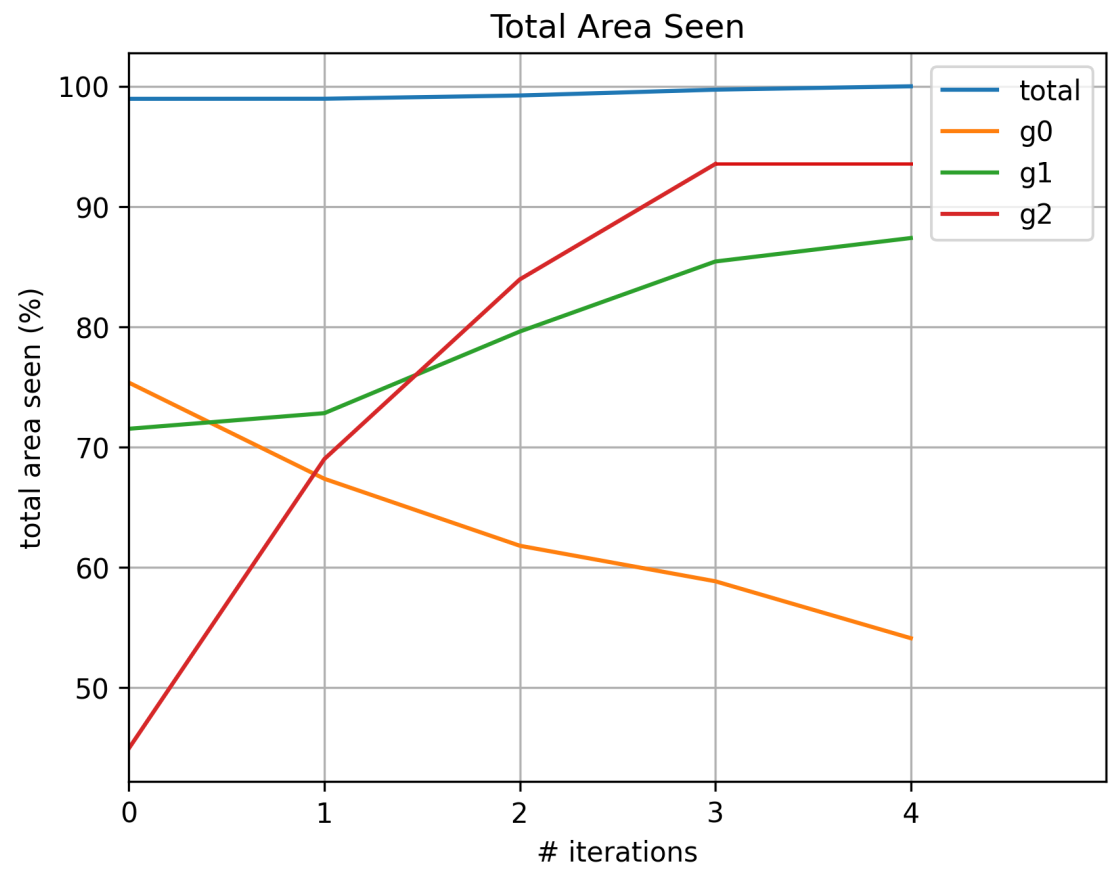
\includegraphics[width = \textwidth]{experiments/area_random_all_fixed2.png}
%         \caption{Seen area for all heuristics.}
%         \label{fig:area_all_pull}
%     \end{subfigure}
%     \hfill
%     \begin{subfigure}{0.45\textwidth}
%         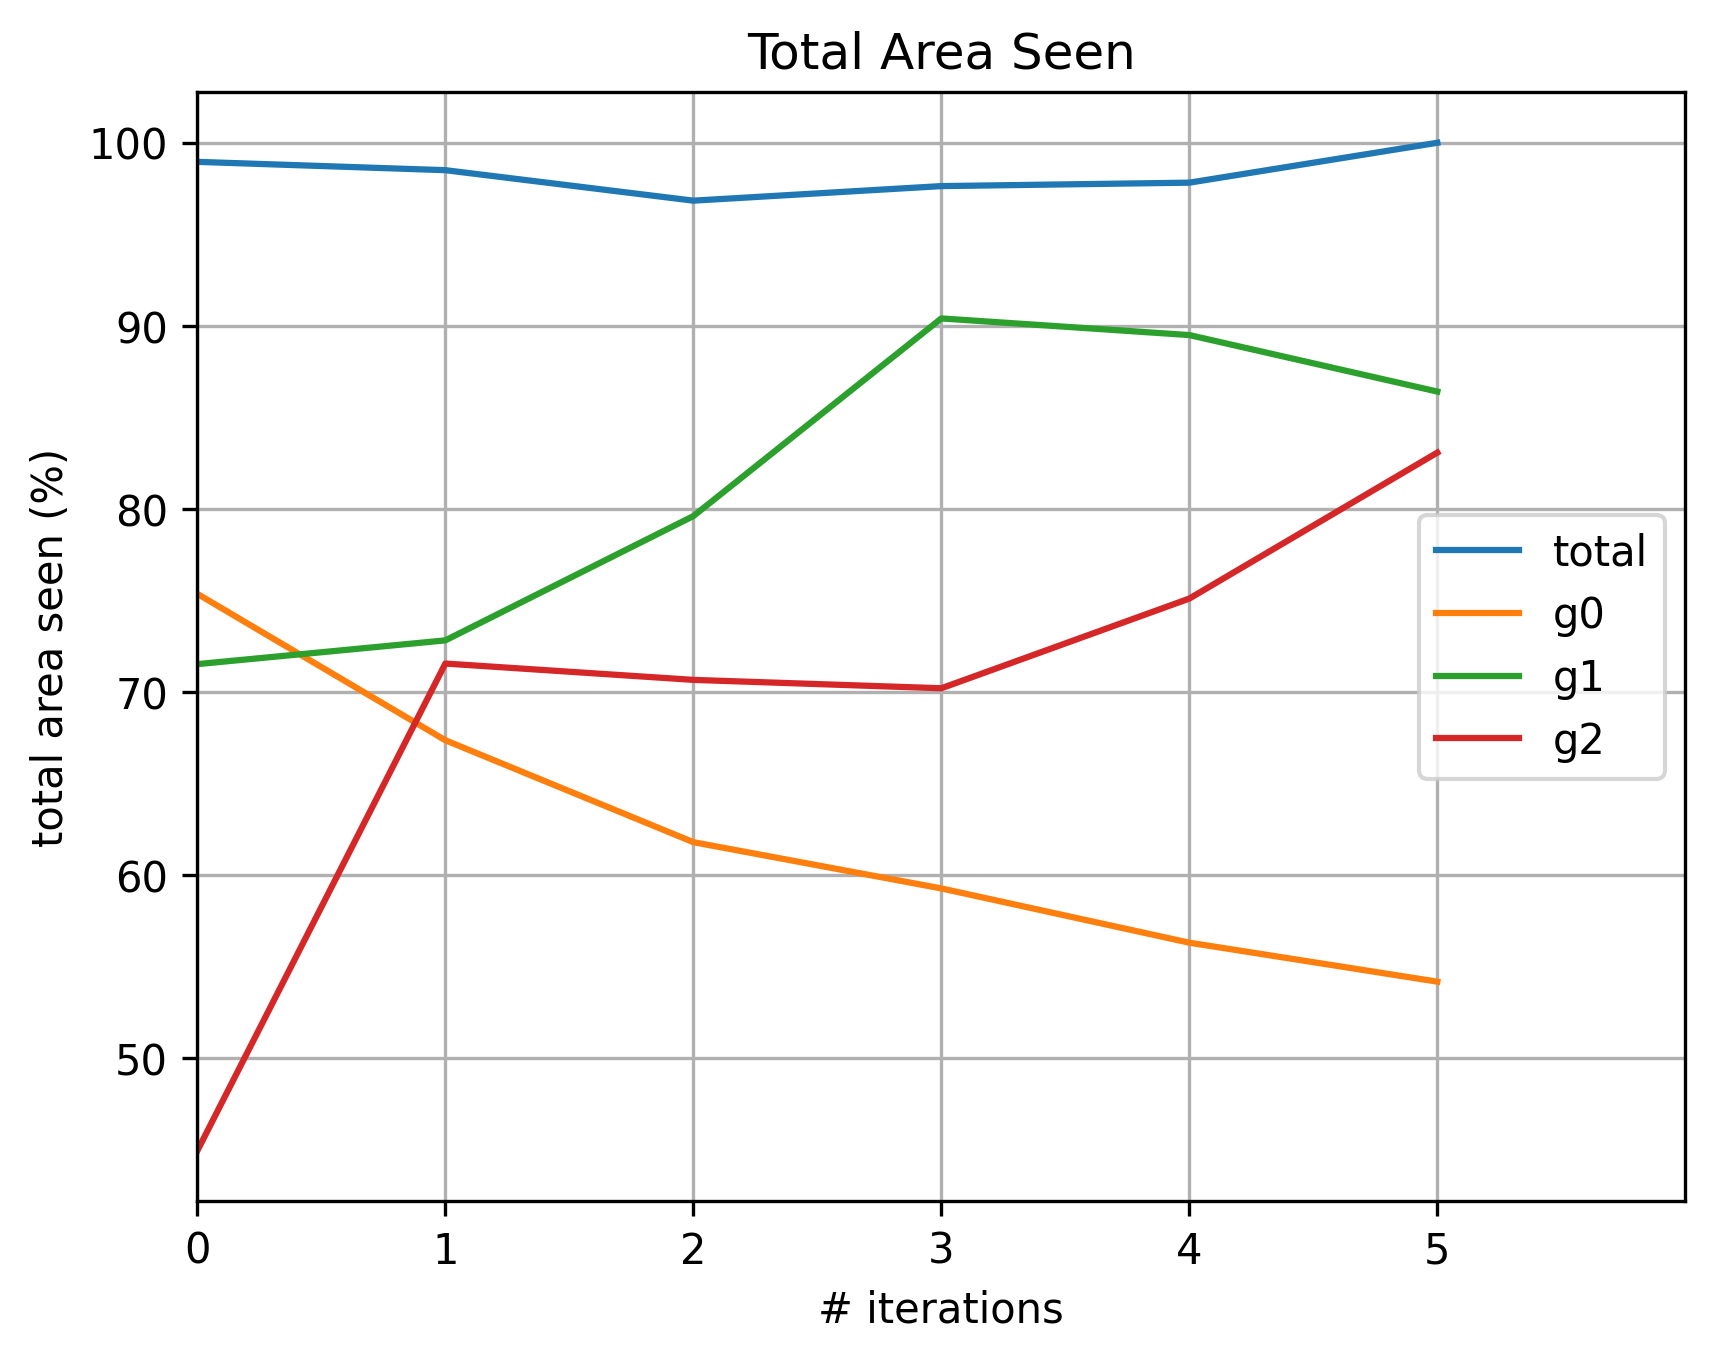
\includegraphics[width = \textwidth]{experiments/area_random_no_pull_fixed.png}
%         \caption{Seen area without pull onto reflex vertices.}
%         \label{fig:area_no_pull}
%     \end{subfigure}
%     \caption{Total and individual areas seen per iteration for an arbitrarily shaped polygon guarded by three guards.}
%     \label{fig:no_pull_plots}
% \end{figure}

\newpage
\subsubsection{Without Pull Capping}
In this section we  discuss how capping the pull towards a reflex vertex influences the progress of the algorithm. Section \ref{sec:pull_capping} introduced the pull capping notion. The reason for this choice was to not allow the pull to overpower the value of the momentum. So, if the pull is larger than $\mu$ times the momentum, it is capped at the momentum value multiplied by $\mu$. 

We  compare how the guards move when we are using all the heuristics to when we are not capping the pull towards reflex vertices. We  use the comb polygon with four teeth as example. The guards have a pull cap hyperparameter $\mu = 1$. Thus, if the pull is larger than the momentum, we cap it at the size of the momentum. This value was chosen experimentally in order to clearly show the benefits of using this heuristic. So, if the pull is as large as the momentum, we prioritise pulling guards onto reflex vertices if they are ``close enough''.


\begin{figure}[h!]
    \centering
    \begin{subfigure}{0.45\textwidth}
        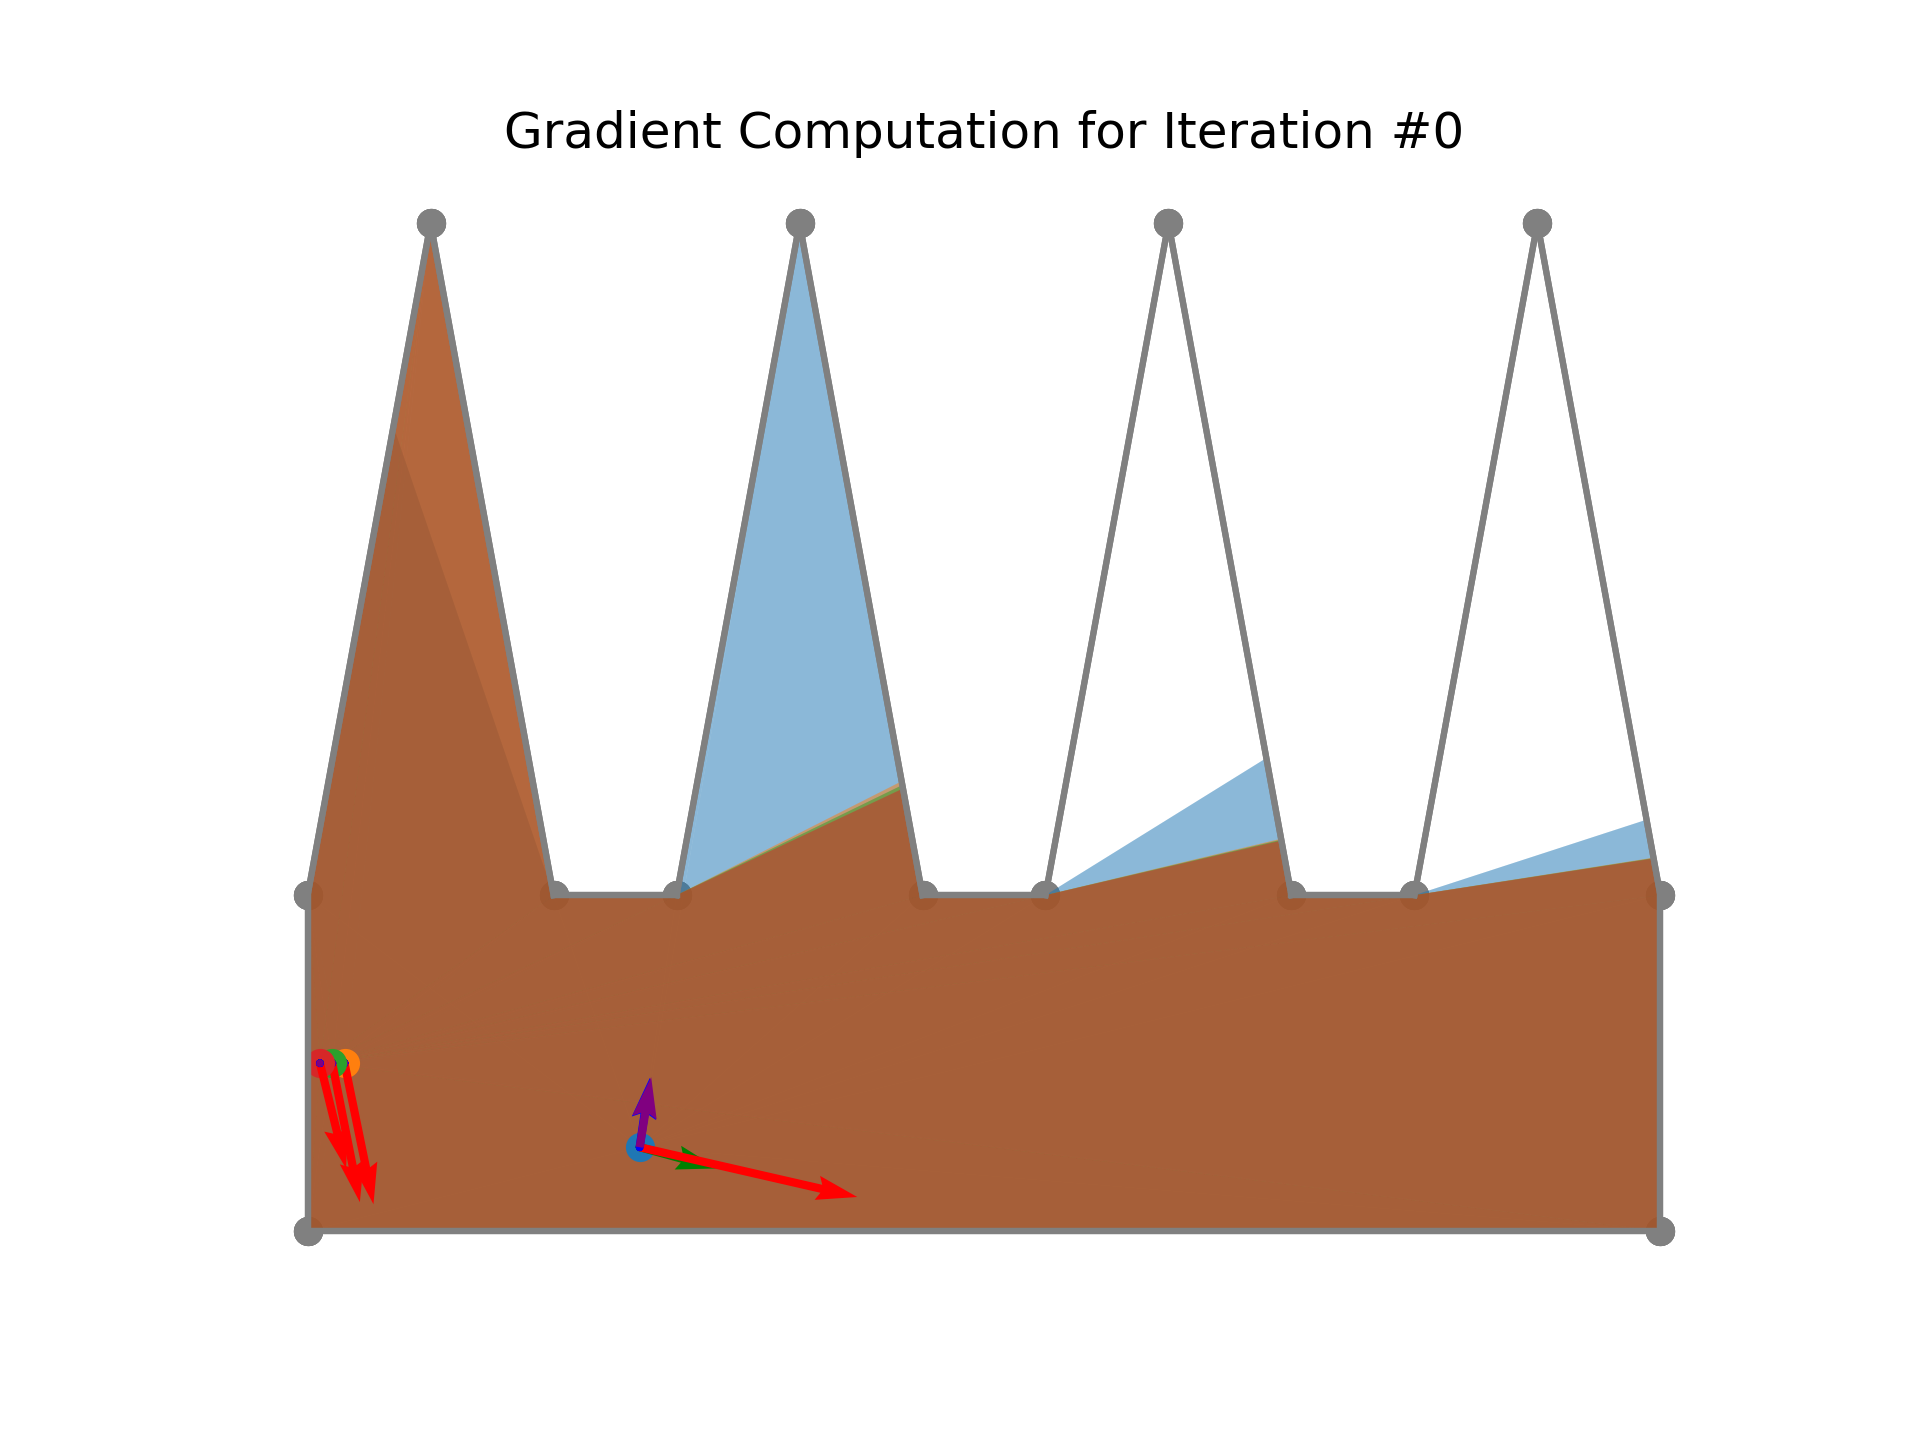
\includegraphics[width = \textwidth]{experiments/comb_capping_pos0.png}
        \caption{All heuristics. The guard's pull towards the reflex vertex is capped.}
        \label{fig:all_cap_pos0}
    \end{subfigure}
    \hfill
    \begin{subfigure}{0.45\textwidth}
        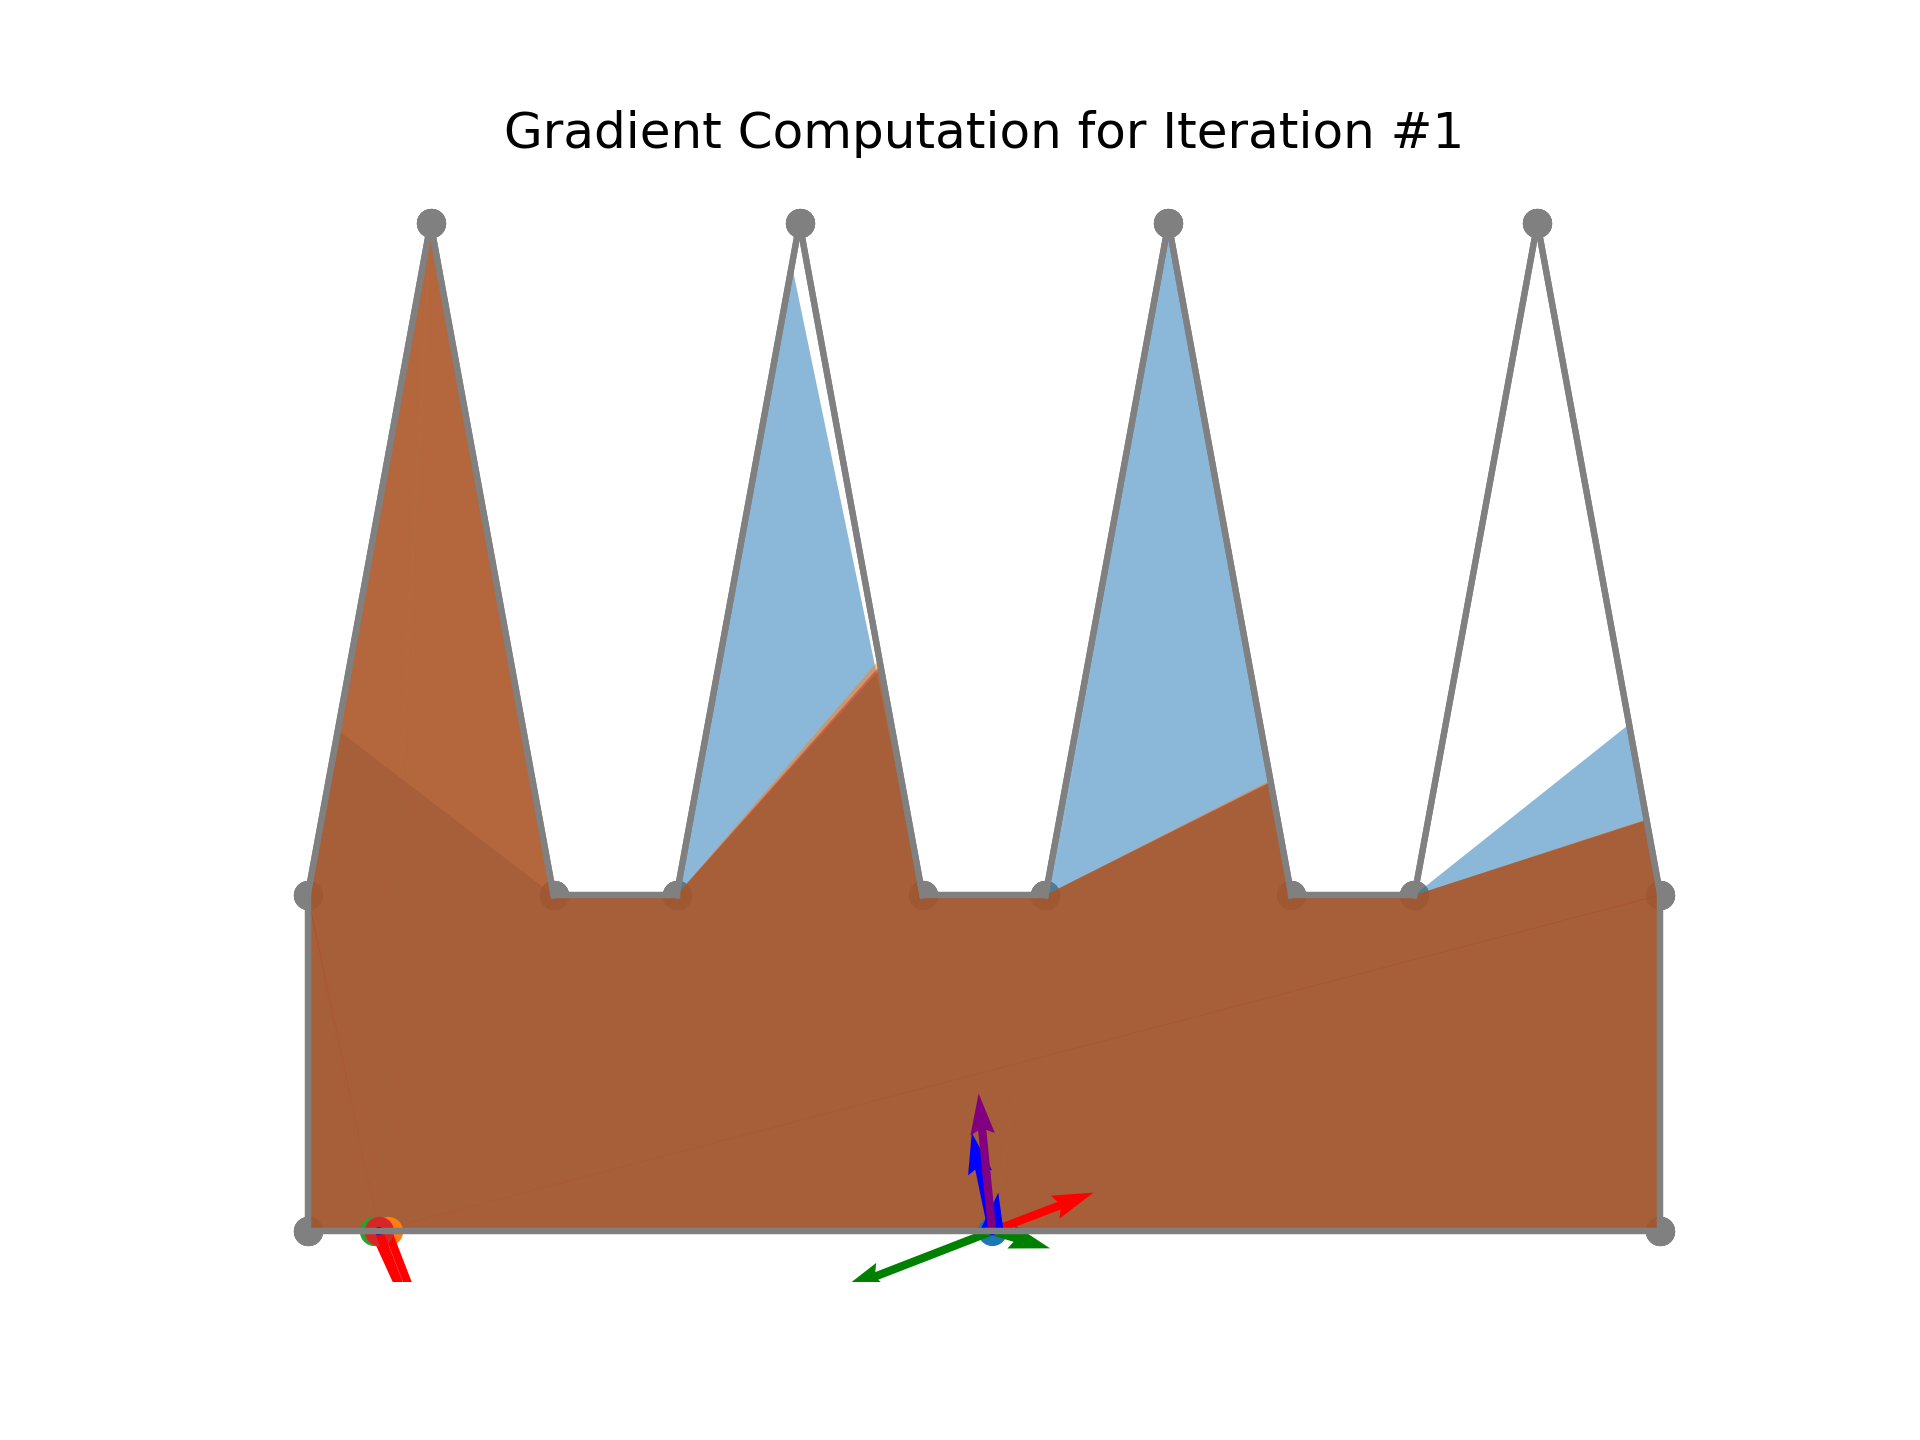
\includegraphics[width = \textwidth]{experiments/comb_capping_pos1.png}
        \caption{All heuristics. The guard does not act upon the pull towards the reflex vertex.}
        \label{fig:all_cap_pos1}
    \end{subfigure}
    \vfill
    \begin{subfigure}{0.45\textwidth}
        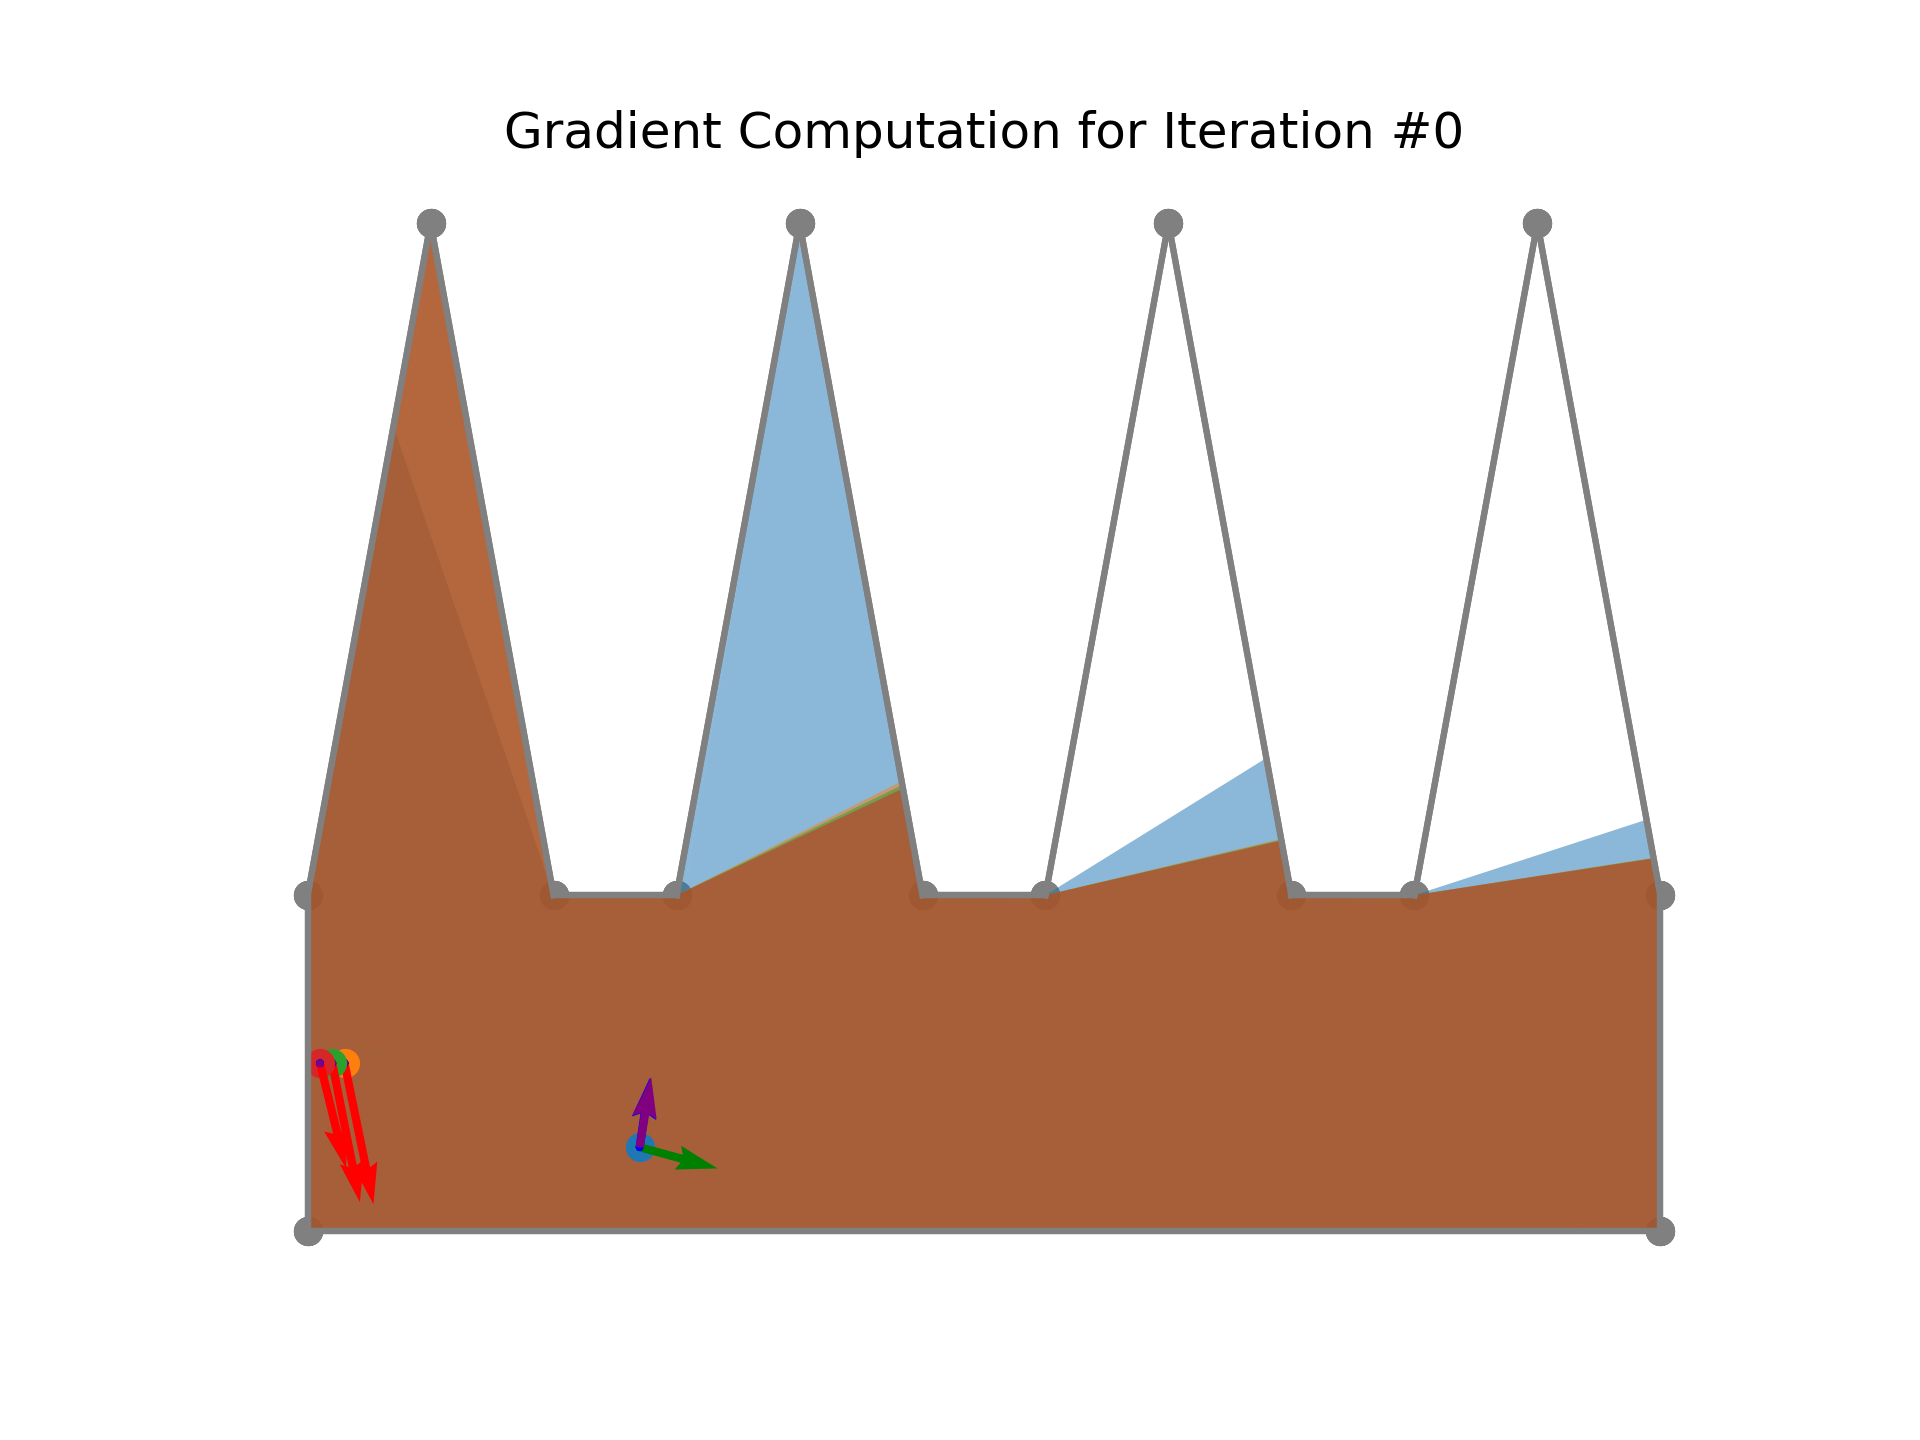
\includegraphics[width = \textwidth]{experiments/comb_no_capping_pos0.png}
        \caption{No pull onto the reflex vertex. The guard's pull towards the reflex vertex is not capped.}
        \label{fig:no_cap_pos0}
    \end{subfigure}
    \hfill
    \begin{subfigure}{0.45\textwidth}
        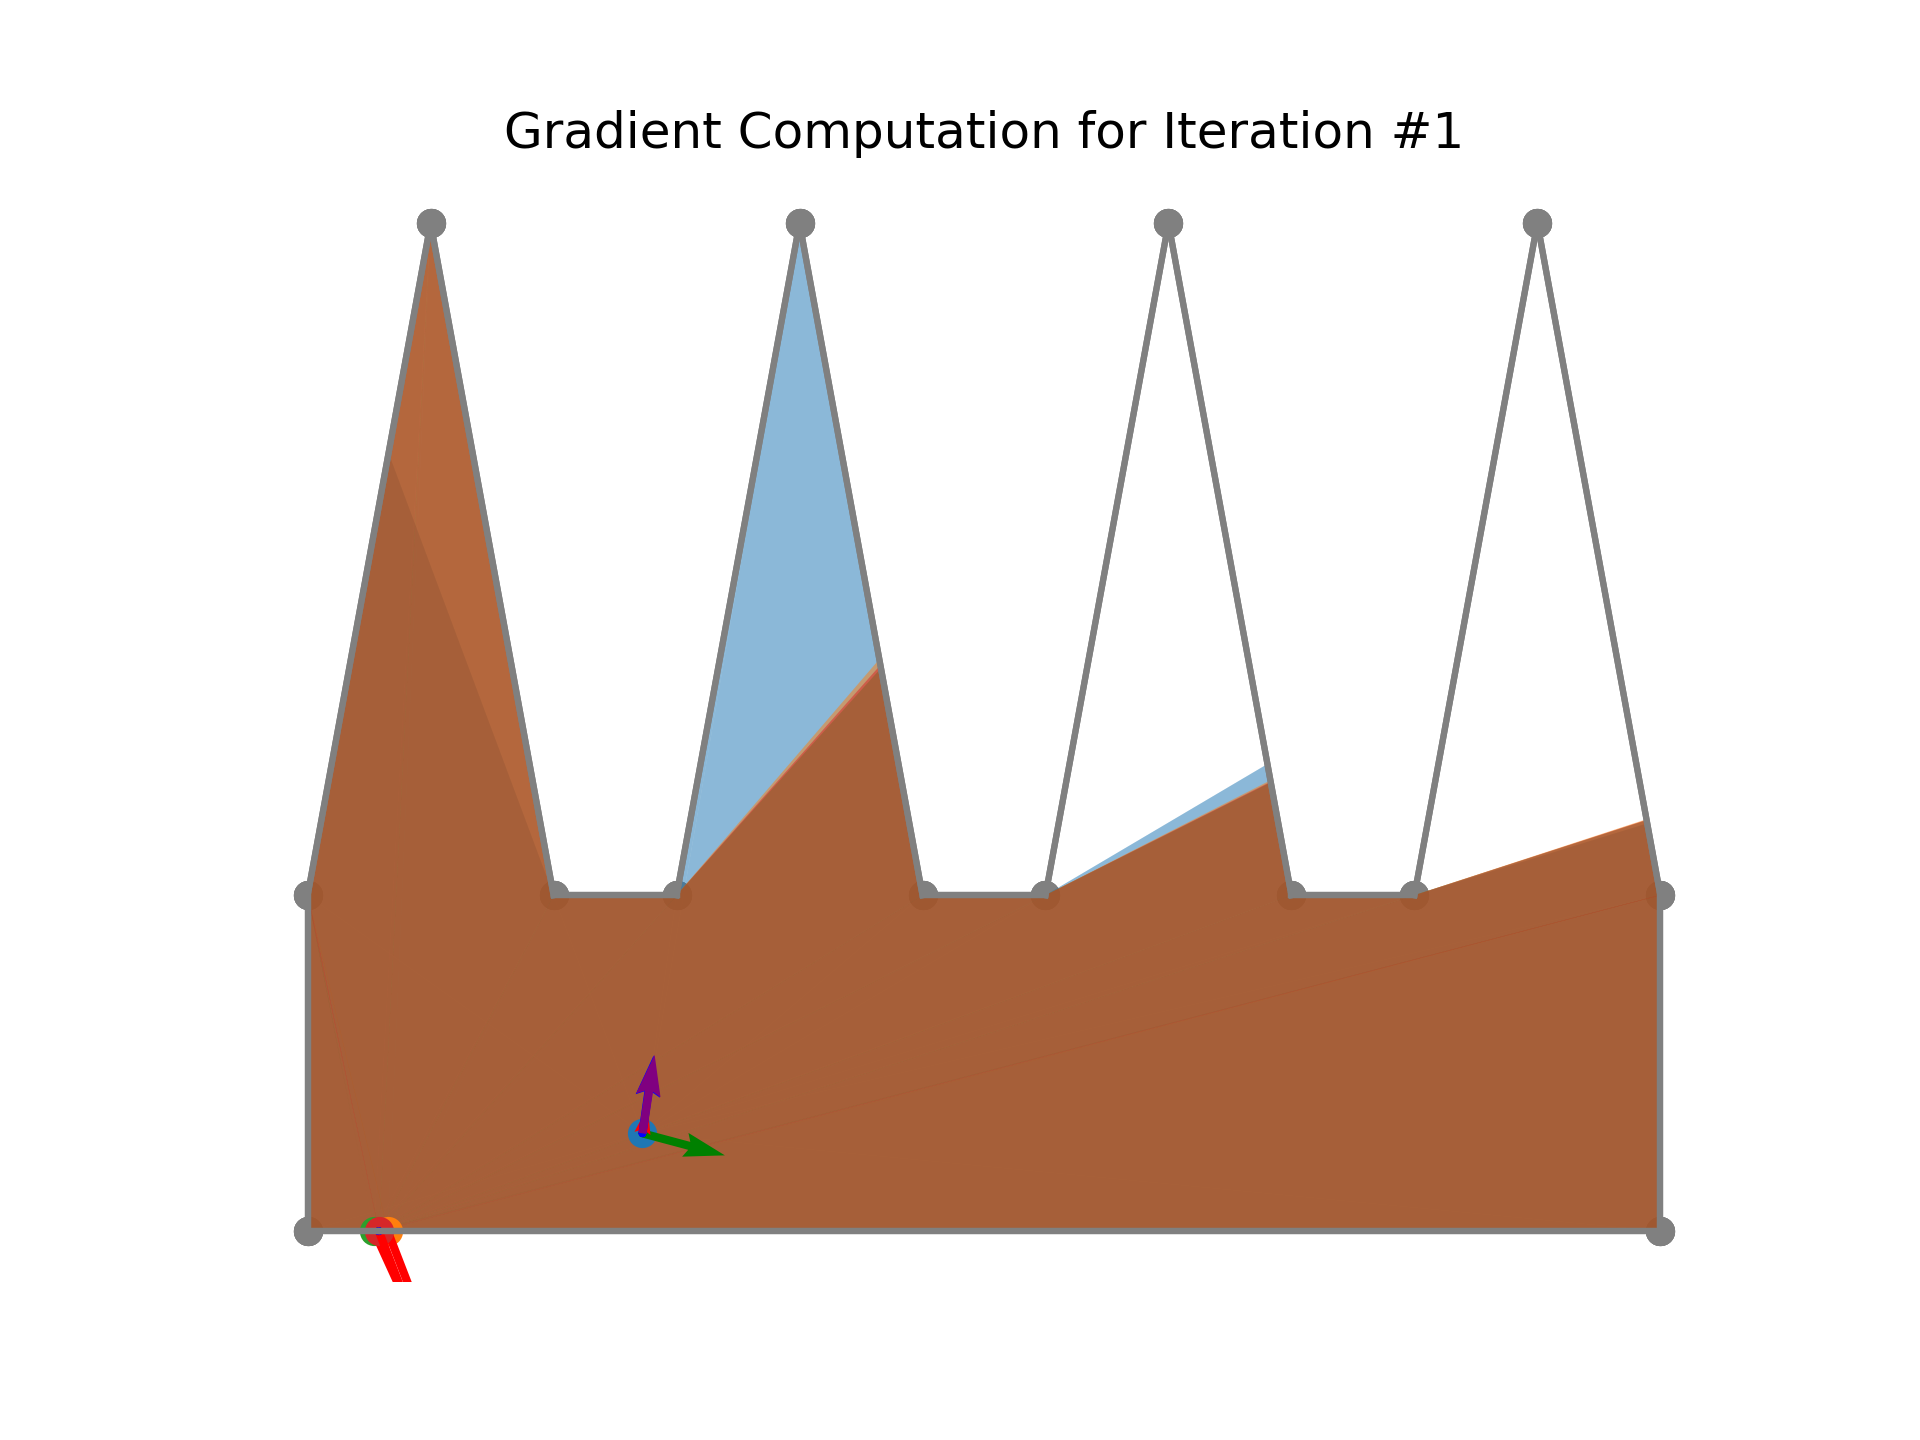
\includegraphics[width = \textwidth]{experiments/comb_no_capping_pos1.png}
        \caption{No pull onto the reflex vertex. The guard is drawn closer to the reflex vertex.}
        \label{fig:no_cap_pos1}
    \end{subfigure}
    \caption{Example of different movements of guards with and without pull capping in a comb polygon with four teeth.}
    \label{fig:no_cap_eg}
\end{figure}

Figure \ref{fig:no_cap_eg} displays the two reflex vertex pull cases: Subfigures \ref{fig:all_cap_pos0} and \ref{fig:all_cap_pos1} show how the blue guard movement changes when its pull is capped; Subfigures \ref{fig:no_cap_pos0} and \ref{fig:no_cap_pos1} show the blue guard's movement without pull capping. We  observe how in Subfigure \ref{fig:all_cap_pos0} the blue guard has its pull towards the reflex vertex capped. In that case, the movement vector is larger than the pull, so the guard doesn't move towards the reflex vertex. So, the blue guard moves as its movement vector dictates to the position in Subfigure \ref{fig:all_cap_pos1}. This encourages the guard to explore the polygon more rather than directly moving towards a reflex vertex.
Conversely, Subfigure \ref{fig:no_cap_pos1} displays the blue guard moving closer to the reflex vertex it is pulled to. In subsequent iterations, it is placed on the reflex vertex.

% \newpage
Figure \ref{fig:no_cap_plots} shows how the global behaviour of the algorithm is influenced by the capping. Interestingly enough, when capping the pull, the guards' behaviour is more erratic. This results in more iterations before the whole polygon is seen (Subfigure \ref{fig:area_all_cap}).  On the other hand, using no capping allows a steadier increase in the total area seen (Subfigure \ref{fig:area_no_cap}). Eventually, the blue guard ($g0$) is drawn and placed onto the reflex vertex in iteration 2. It is worth mentioning that it does not move in the last iteration because the other guards have already covered the whole polygon. Nonetheless, the reflex vertex placement does not improve the locally seen area. It however reinforces the previously discussed idea that placing guards on reflex vertices is globally beneficial for the algorithm. As such, tuning the hyperparameter $\mu$ is a crucial point of exploration for deciding how and when pull capping would always prove most favourable.

\begin{figure}[!h]
    \begin{subfigure}{0.45\textwidth}
        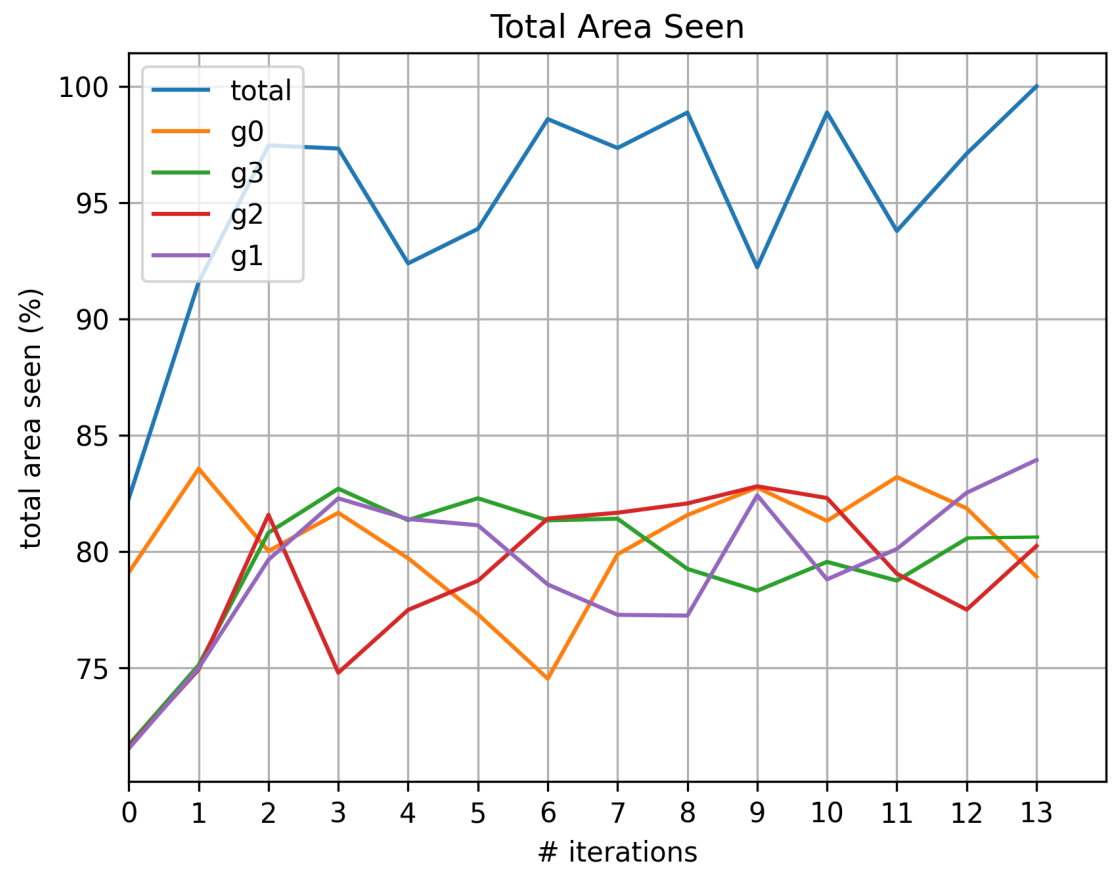
\includegraphics[width = \textwidth]{experiments/area_comb_capping2.png}
        \caption{Seen area for all heuristics.}
        \label{fig:area_all_cap}
    \end{subfigure}
    \hfill
    \begin{subfigure}{0.45\textwidth}
        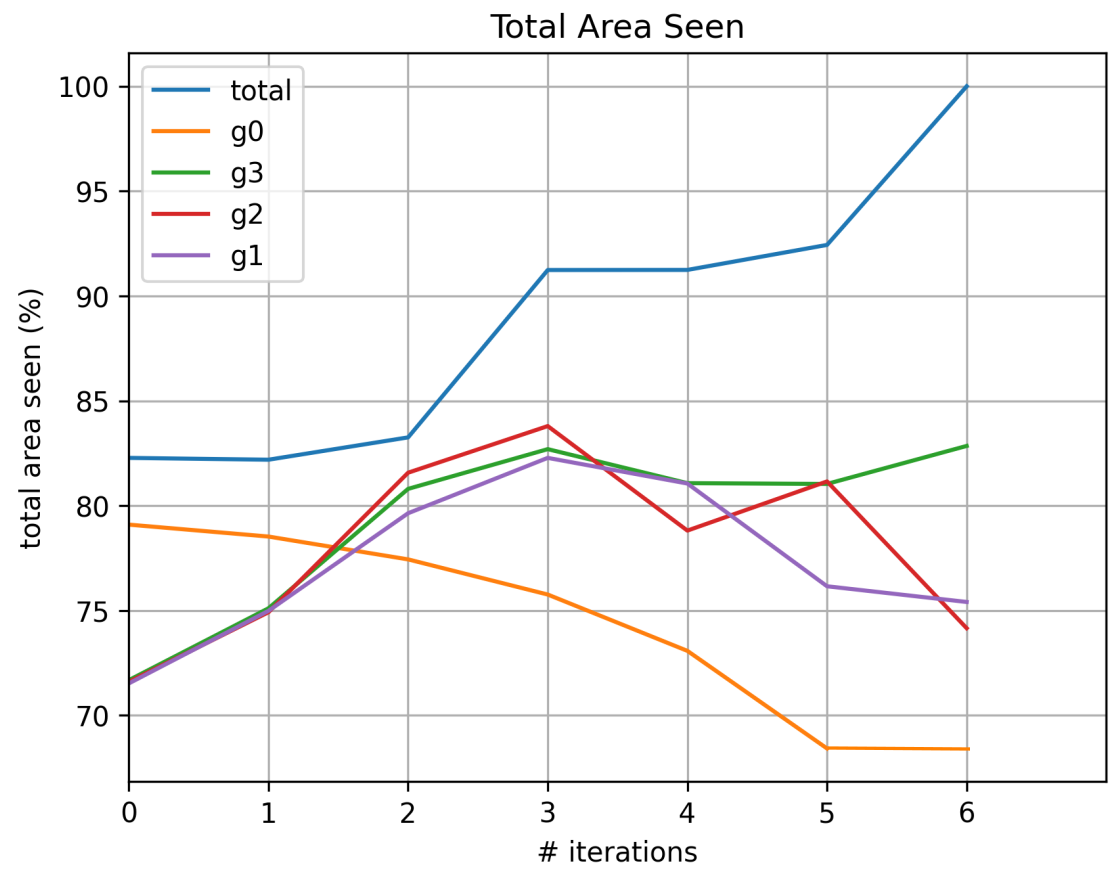
\includegraphics[width = \textwidth]{experiments/area_comb_no_capping2.png}
        \caption{Seen area without pull capping.}
        \label{fig:area_no_cap}
    \end{subfigure}
    \caption{Total and individual areas seen per iteration for a comb polygon with four teeth.}
    \label{fig:no_cap_plots}
\end{figure}

In this way, we claim that capping the guards' pull towards a reflex vertex highly depends on the hyperparameter $\mu$. When not capped, it emphasises the importance of placing guards on reflex vertices. However, when the pull of guards is capped, we are using a more exploratory approach to discovering the polygon. Thus, we can experimentally decide whether to use this heuristic. 
% The shape of the polygon can influence this decision as well.

\newpage
\subsubsection{Without Reflex Area}
In this section we  discuss the importance of keeping guards in the reflex area of a reflex vertex they had been placed on. Section \ref{sec:reflex_area} introduced this heuristic. The idea counteracts the edge-case of guards moving away from reflex vertices they had been placed on. When they move away from the reflex vertex, they might unsee a large previously seen area. It is possible that afterwards their movement vector directs them to move back onto the reflex vertex. We want to prevent them from unnecessarily moving away and then back on the vertex in a loop. For this reason, we  keep them in the reflex area. The reflex area is then the area determined by the two segment lines meeting in the reflex vertex. By staying in this area, the guard would be able to move away from the reflex vertex in a direction that does not undo its progress.

% \newpage
We  compare how the guards move when we are using all the heuristics to when we are not keeping guards into a reflex area. We  use another arbitrary polygon as an example, that needs two guards to be fully seen.

Figures \ref{fig:reflex_area_eg} and \ref{fig:area_reflex_area} compare the algorithm progress when using and not using the reflex area heuristic, respectively. Subfigures \ref{fig:reflex_area_all1} - \ref{fig:reflex_area_all4} show the guards' movement when one of them is bound to the reflex area. In this case, the blue guard wants to move away from the reflex vertex. The reflex area does not allow it to move away from the reflex vertex, so it stays there. 
Subfigures \ref{fig:reflex_area_no1} - \ref{fig:reflex_area_no4} display the guards' movement when the reflex area heuristic is not applied. In this case, the blue guard moves away from the reflex vertex (Subfigure \ref{fig:reflex_area_no2}), only to be drawn back to it in the next iteration (Subfigure \ref{fig:reflex_area_no3}). This repetitive behaviour continues without eventually reaching the optimum state.

% \newpage
Figure \ref{fig:area_reflex_area} displays the difference in the areas seen between the two approaches. When using all heuristics (Subfigure \ref{fig:area_reflex_area_all}), the algorithm terminates in 7 iterations. The continuous line marks the guard who did not move away from the reflex vertex. Conversely, when not using the reflex area heuristic (Subfigure \ref{fig:area_reflex_area_no}), the algorithm appears not to terminate. One of the guards loops away and back on the reflex vertex. The other guard loops so that it sees the area that is being seen and unseen by the other guard. In this way, they do not synchronise in order to see the polygon at the same time. This shows in the repetitive plot.

In this way, the reflex area heuristic becomes important to the correct run of the algorithm. It addresses the issue of guards moving repeatedly away and back on reflex vertices. This behaviour causes the other guards to move towards the area that becomes unseen by the first guard. The guards continue to move out of sync with each other, resulting in the polygon never being fully seen.

\newpage
% \thispagestyle{empty}
\begin{figure}[h!]
    \centering
    % \begin{resizebox}{\linewidth}{!}{
    \begin{adjustbox}{minipage=\textwidth,scale=0.9}
        \begin{subfigure}{0.45\textwidth}
            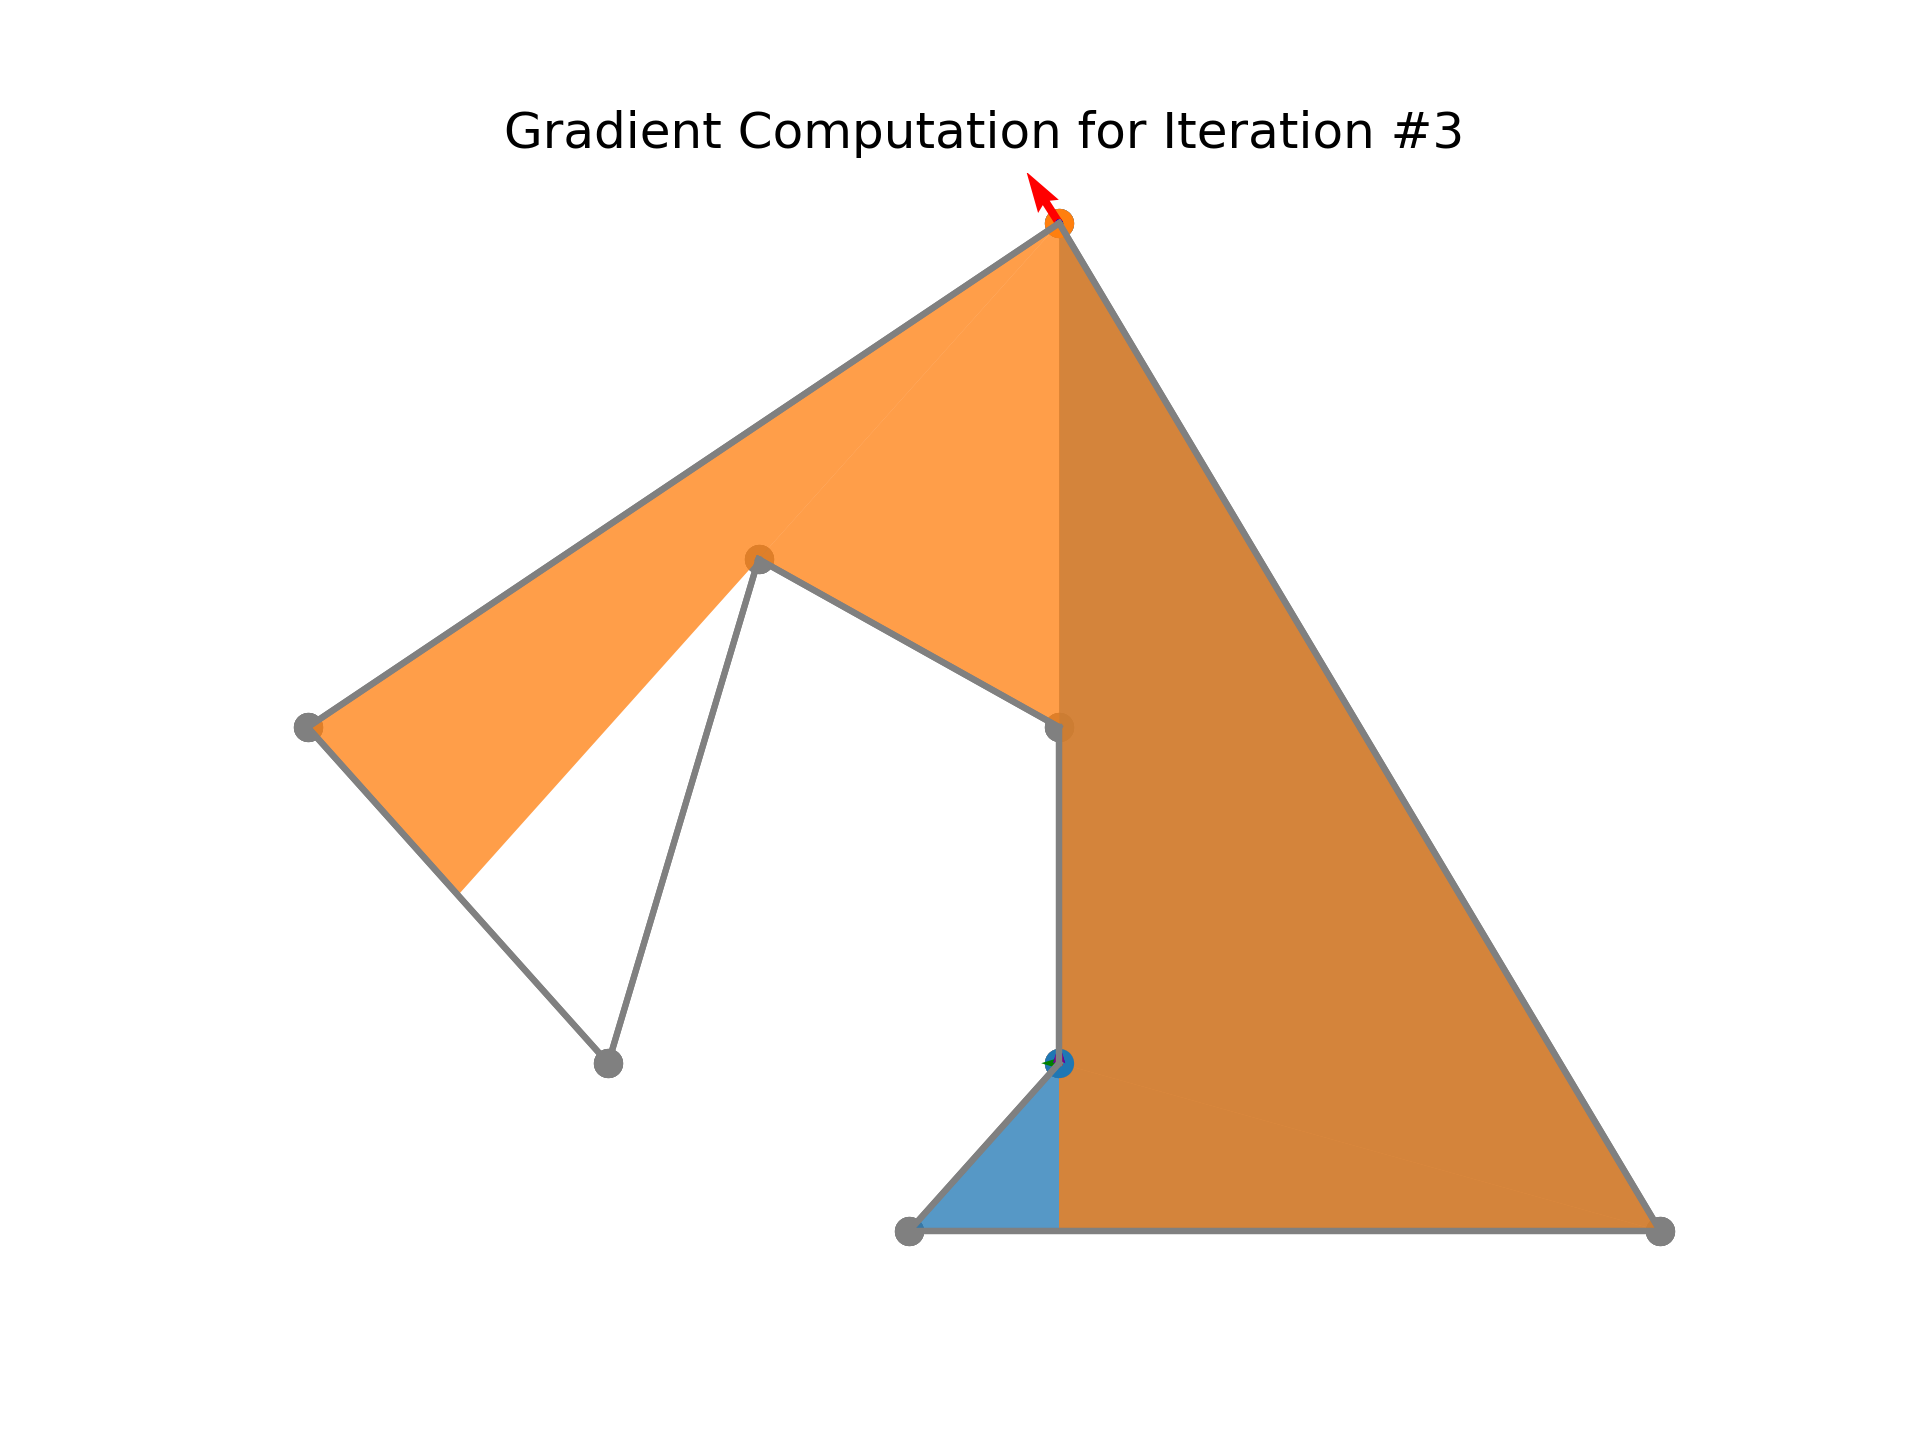
\includegraphics[width = \textwidth]{experiments/reflex_area_all_pos3.png}
            \caption{All heuristics. The blue guard is on the reflex vertex.}
            \label{fig:reflex_area_all1}
        \end{subfigure}
        \hfill
        \begin{subfigure}{0.45\textwidth}
            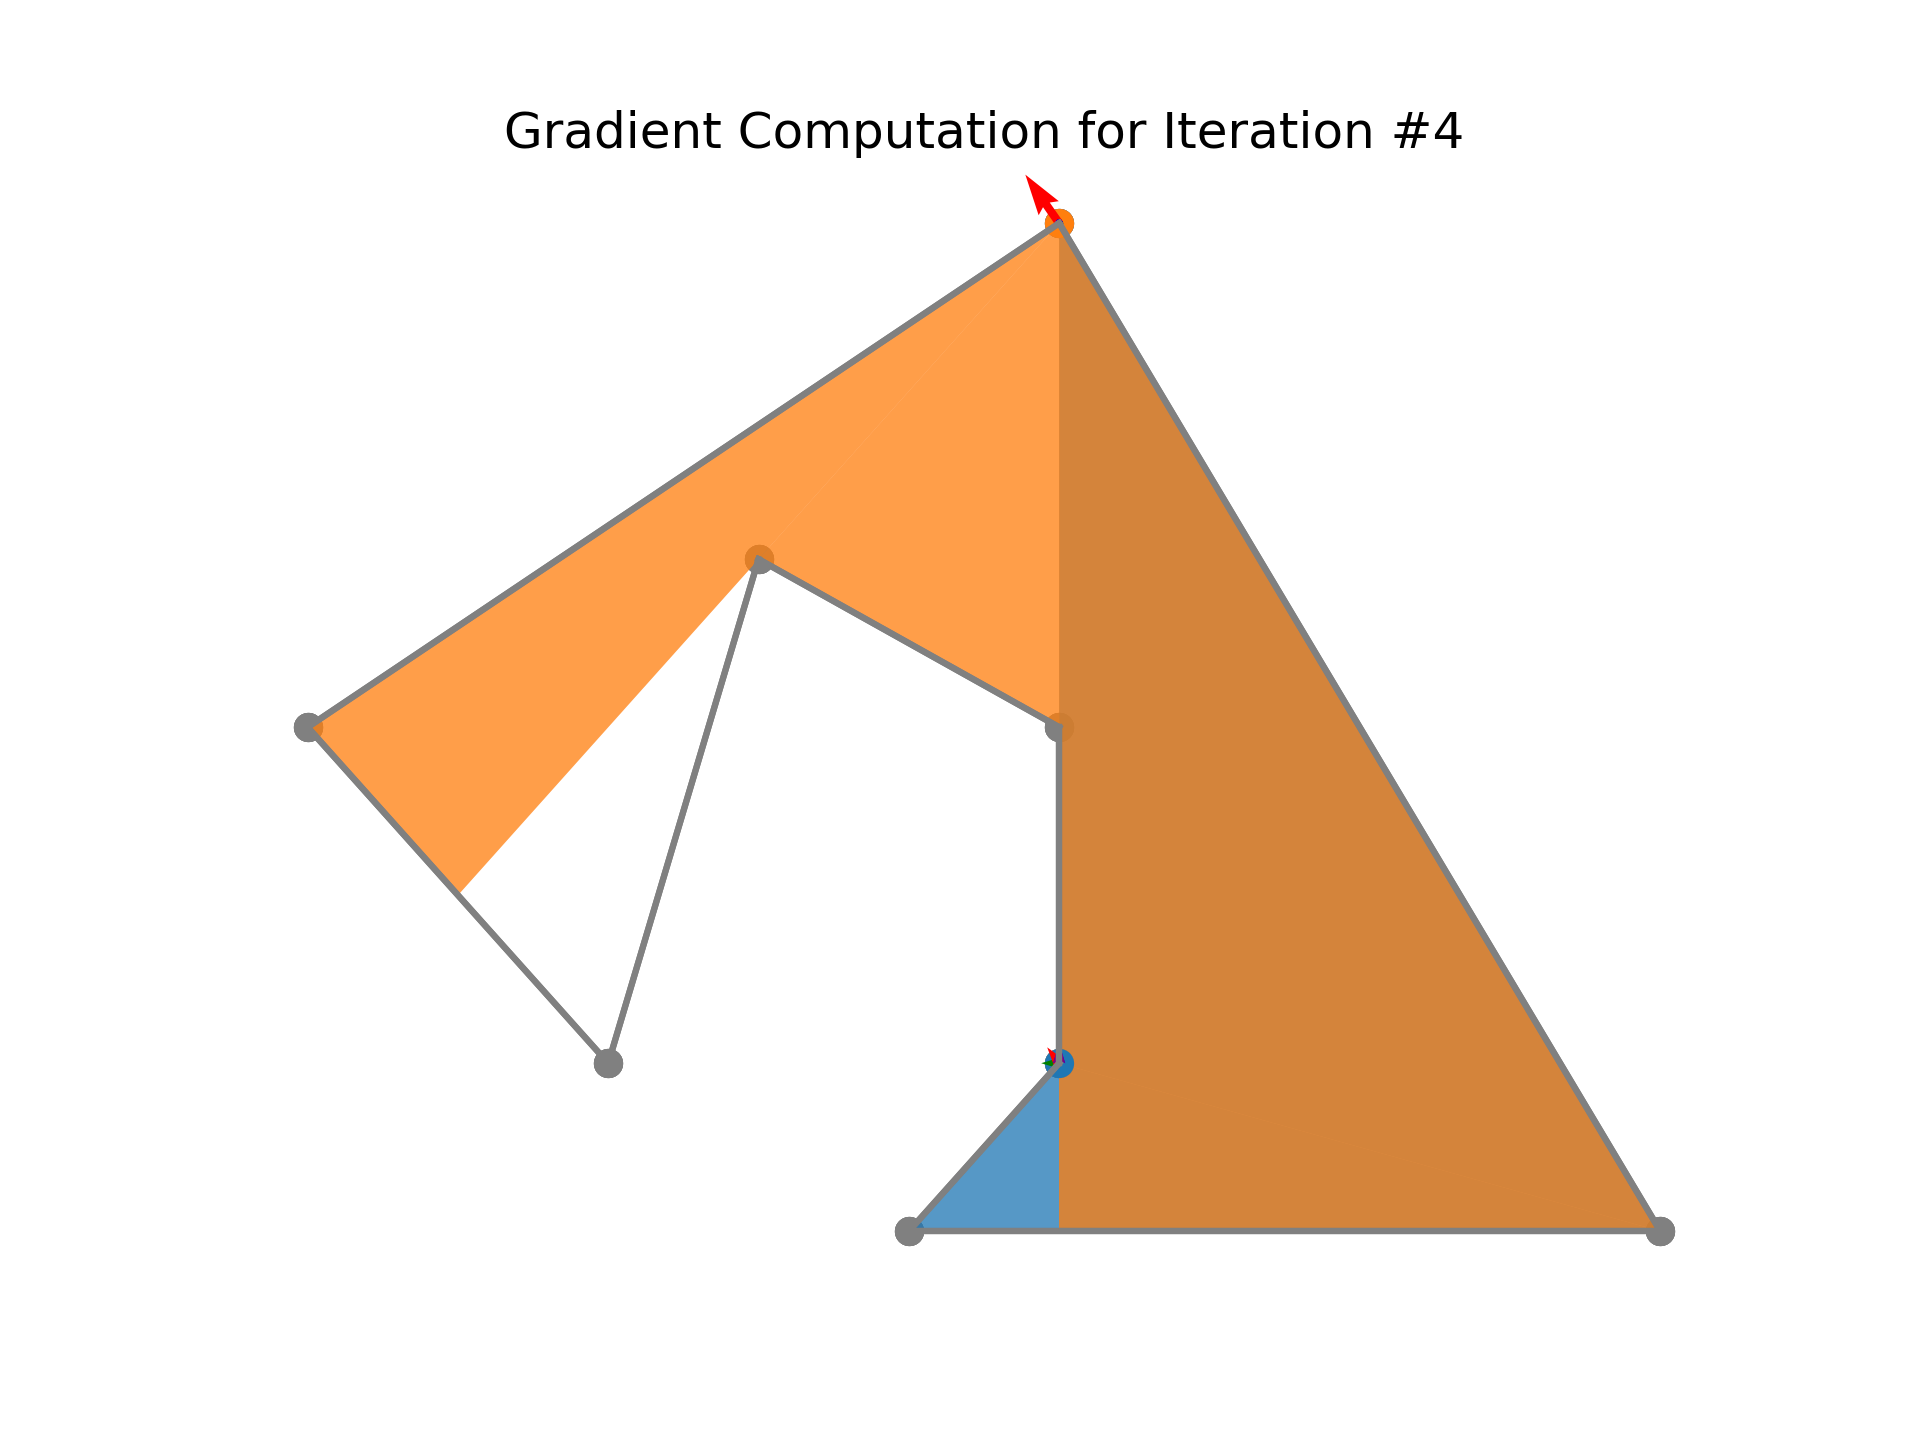
\includegraphics[width = \textwidth]{experiments/reflex_area_no_pos4.png}
            \caption{No reflex area. The blue guard is on the reflex vertex.}
            \label{fig:reflex_area_no1}
        \end{subfigure}
        % \hfill
        \begin{subfigure}{0.45\textwidth}
            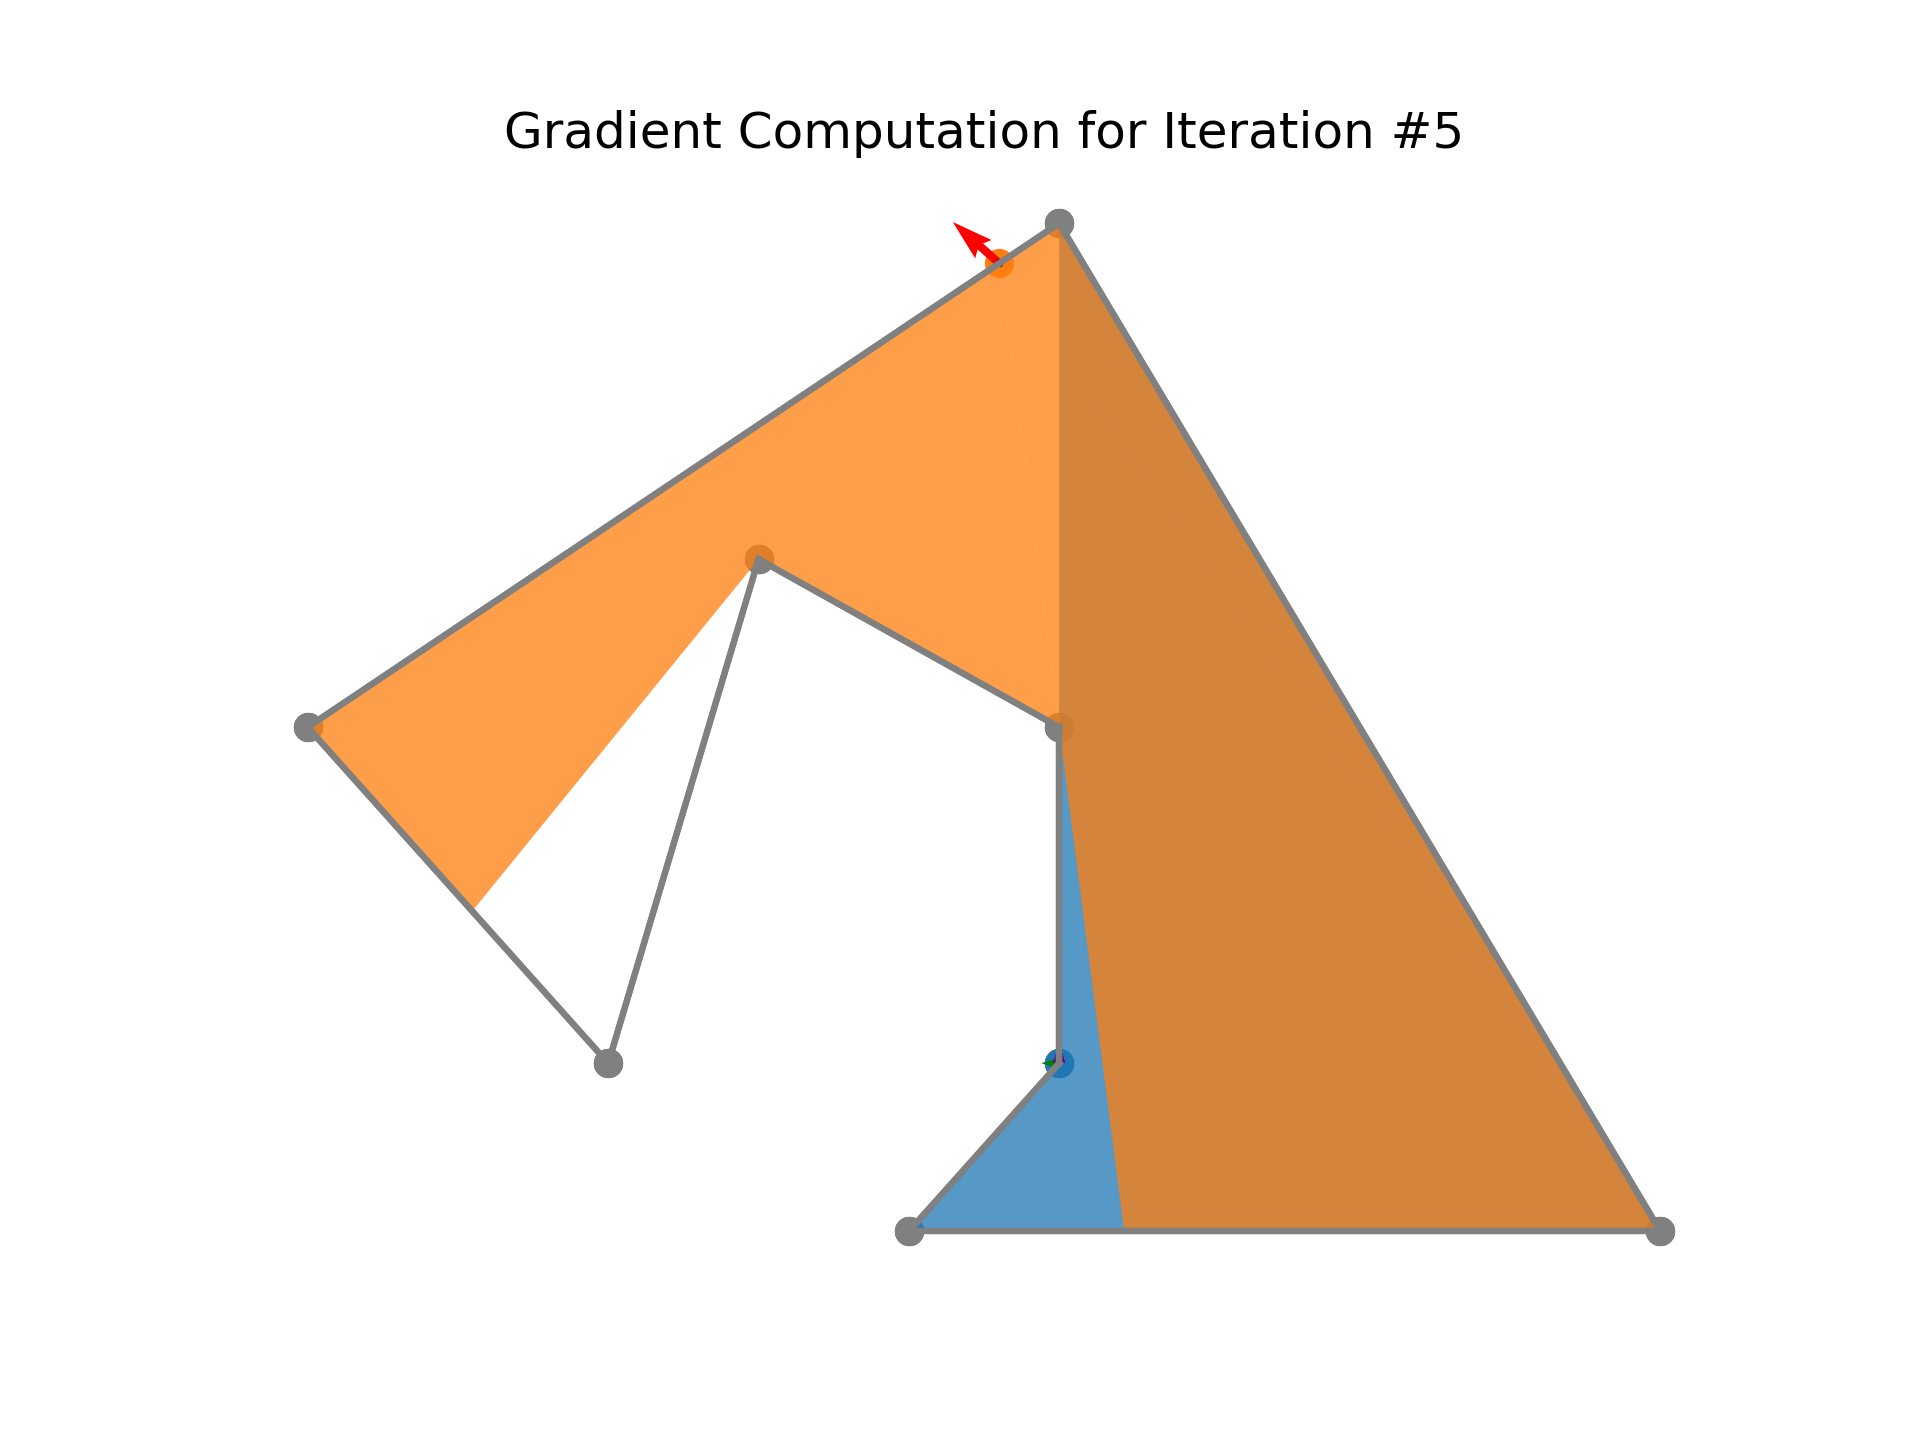
\includegraphics[width = \textwidth]{experiments/reflex_area_all_pos5.png}
            \caption{All heuristics. The blue guard is still on the reflex vertex (in the reflex area).}
        \end{subfigure}
        \hfill
        \begin{subfigure}{0.45\textwidth}
            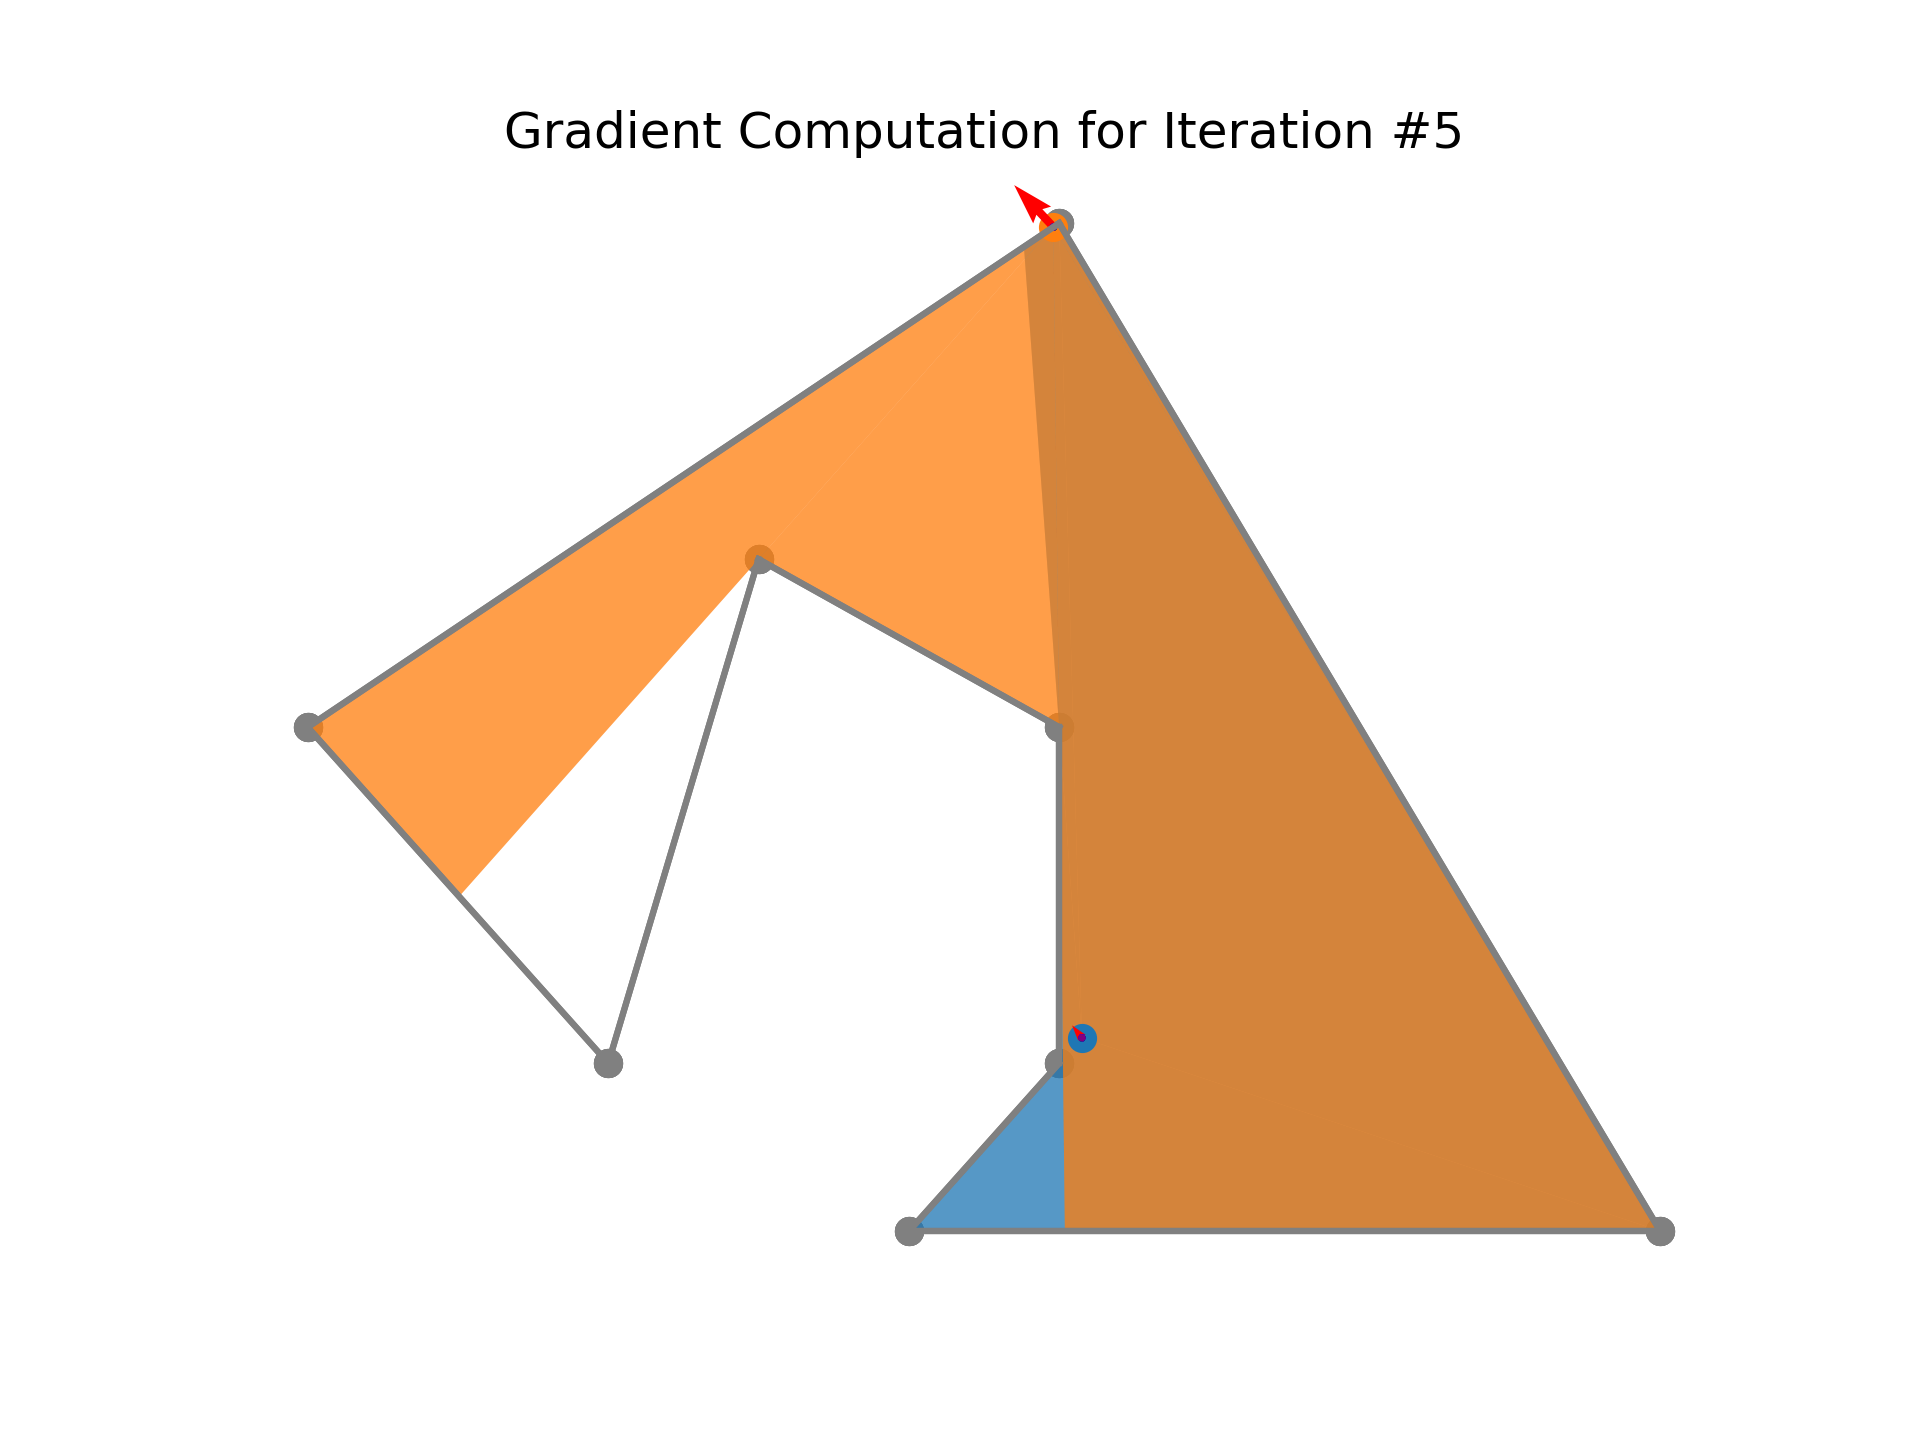
\includegraphics[width = \textwidth]{experiments/reflex_area_no_pos5.png}
            \caption{No reflex area. The blue guard moved away from the reflex vertex.}
            \label{fig:reflex_area_no2}
        \end{subfigure}
        \begin{subfigure}{0.45\textwidth}
            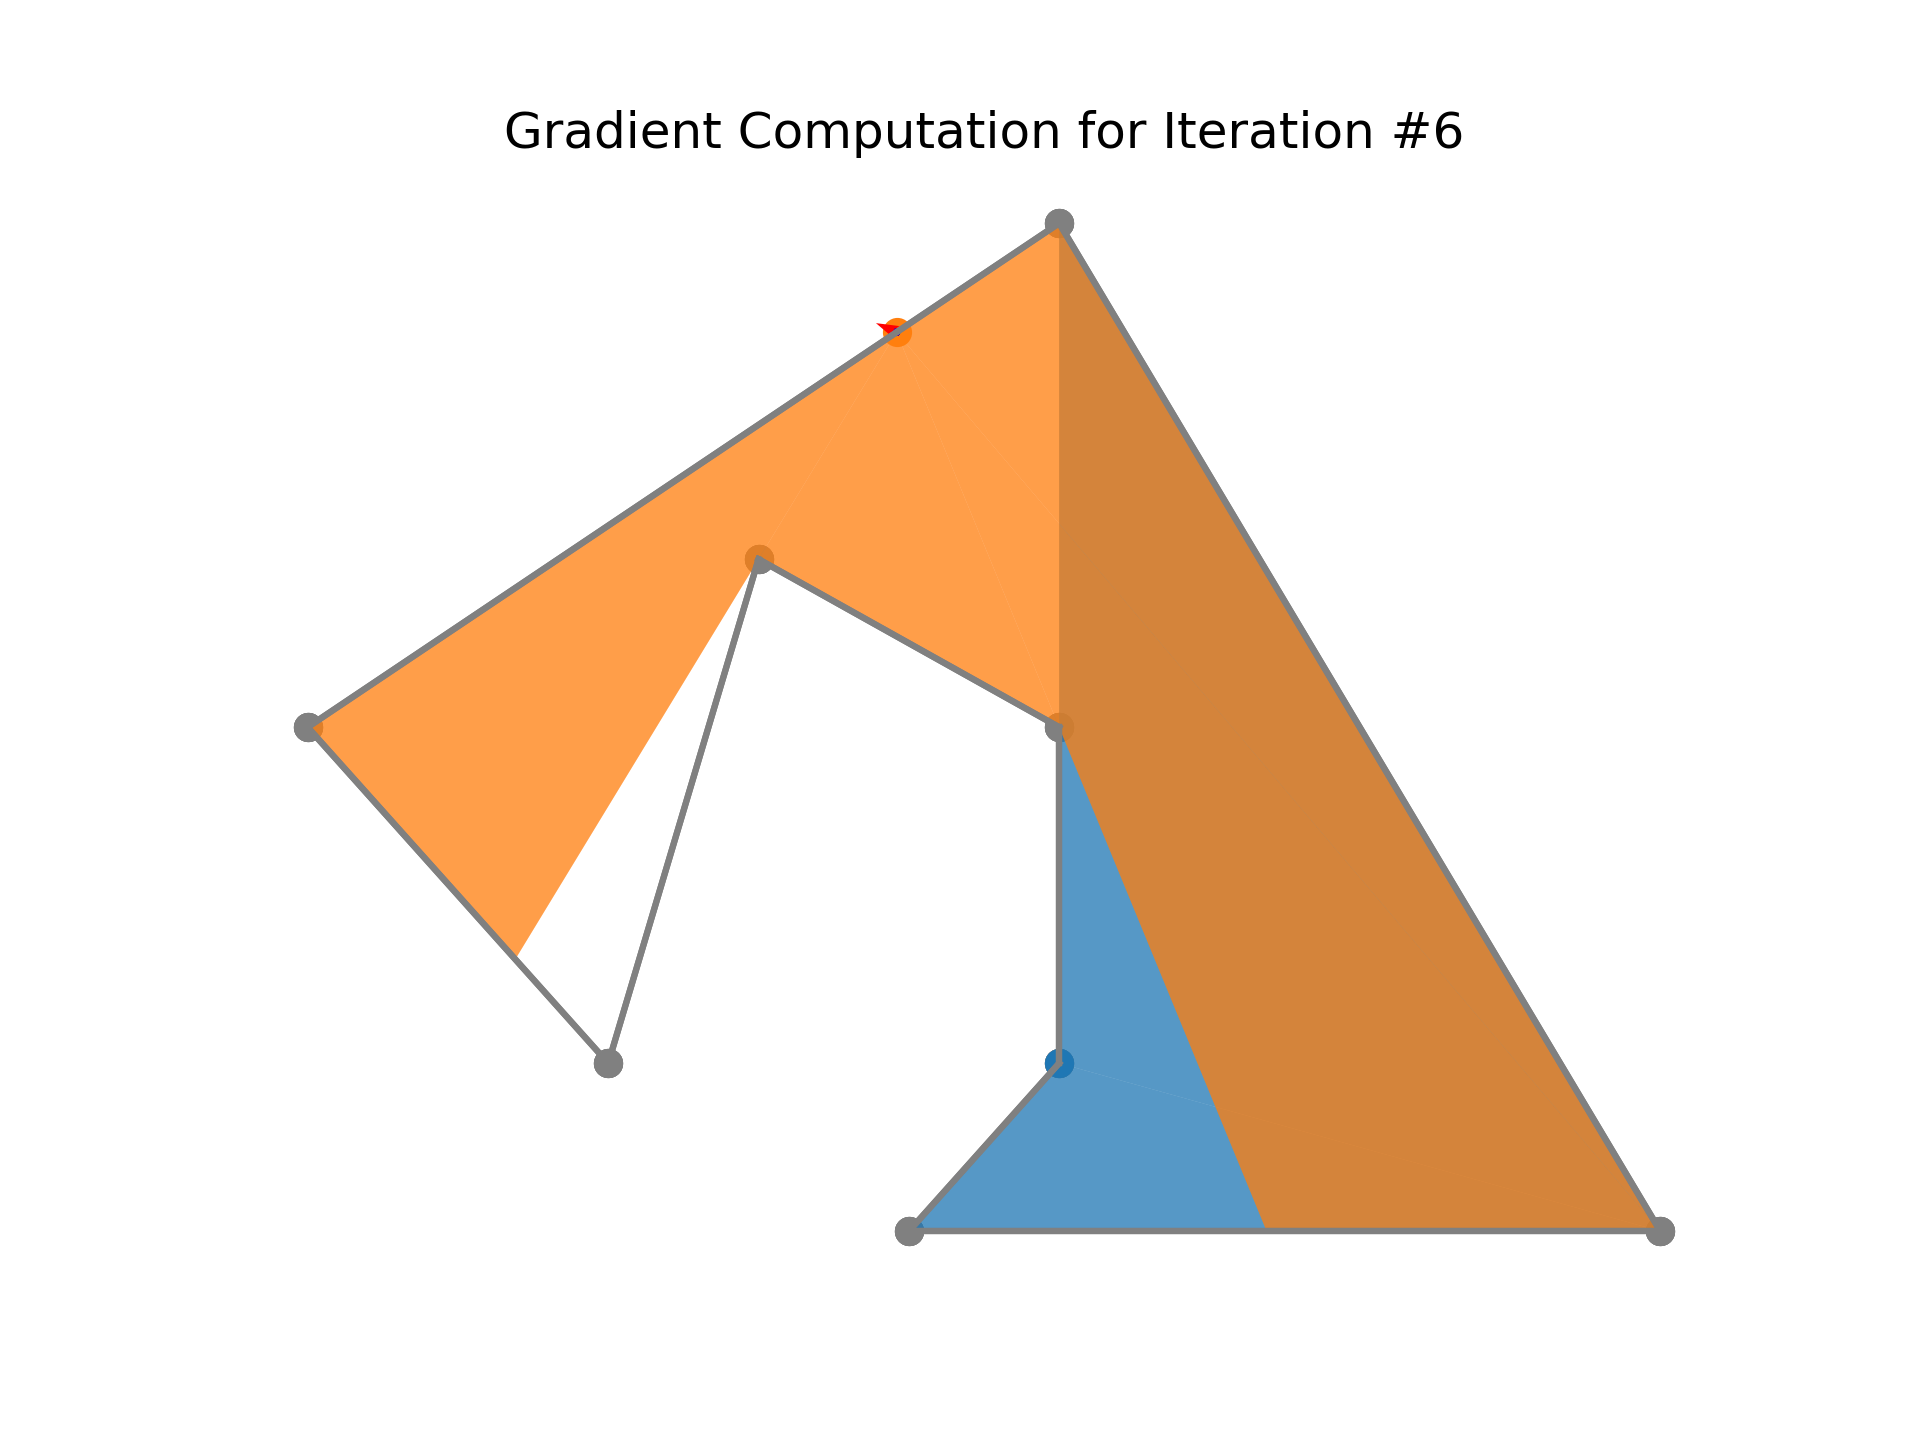
\includegraphics[width = \textwidth]{experiments/reflex_area_all_pos6.png}
            \caption{All heuristics. The blue guard is still on the reflex vertex (in the reflex area).}
            \label{fig:reflex_area_all4}
        \end{subfigure}
        \hfill
        \begin{subfigure}{0.45\textwidth}
            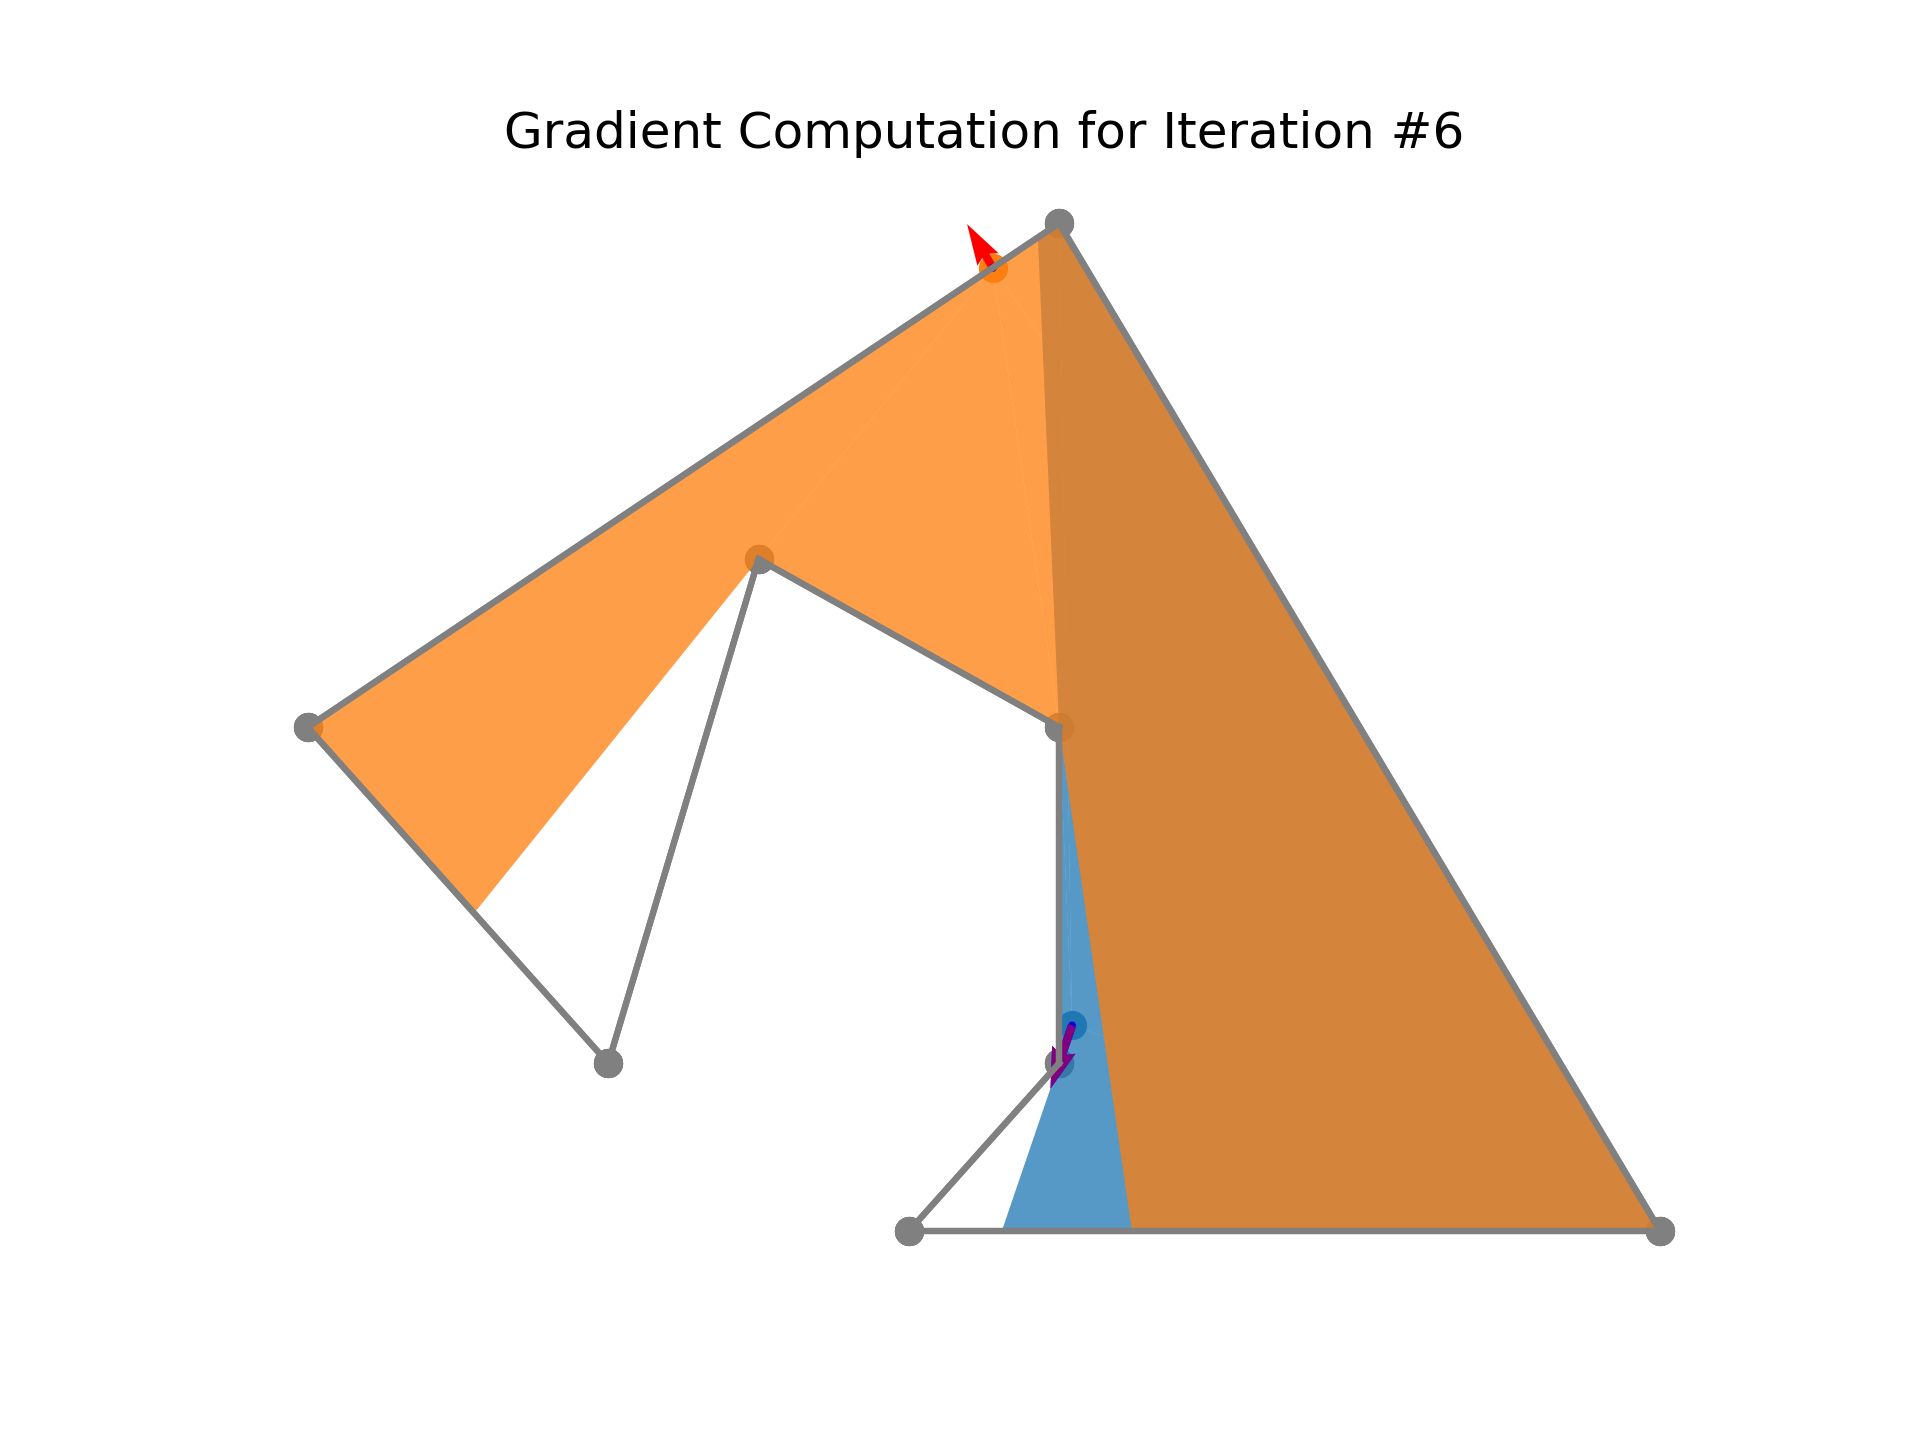
\includegraphics[width = \textwidth]{experiments/reflex_area_no_pos6.png}
            \caption{No reflex area. The blue guard is drawn back to the same reflex vertex.}
            \label{fig:reflex_area_no3}
        \end{subfigure}
    % \end{figure}
    % \begin{figure}
    %     \ContinuedFloat
    %     \centering
        \begin{subfigure}{0.45\textwidth}
            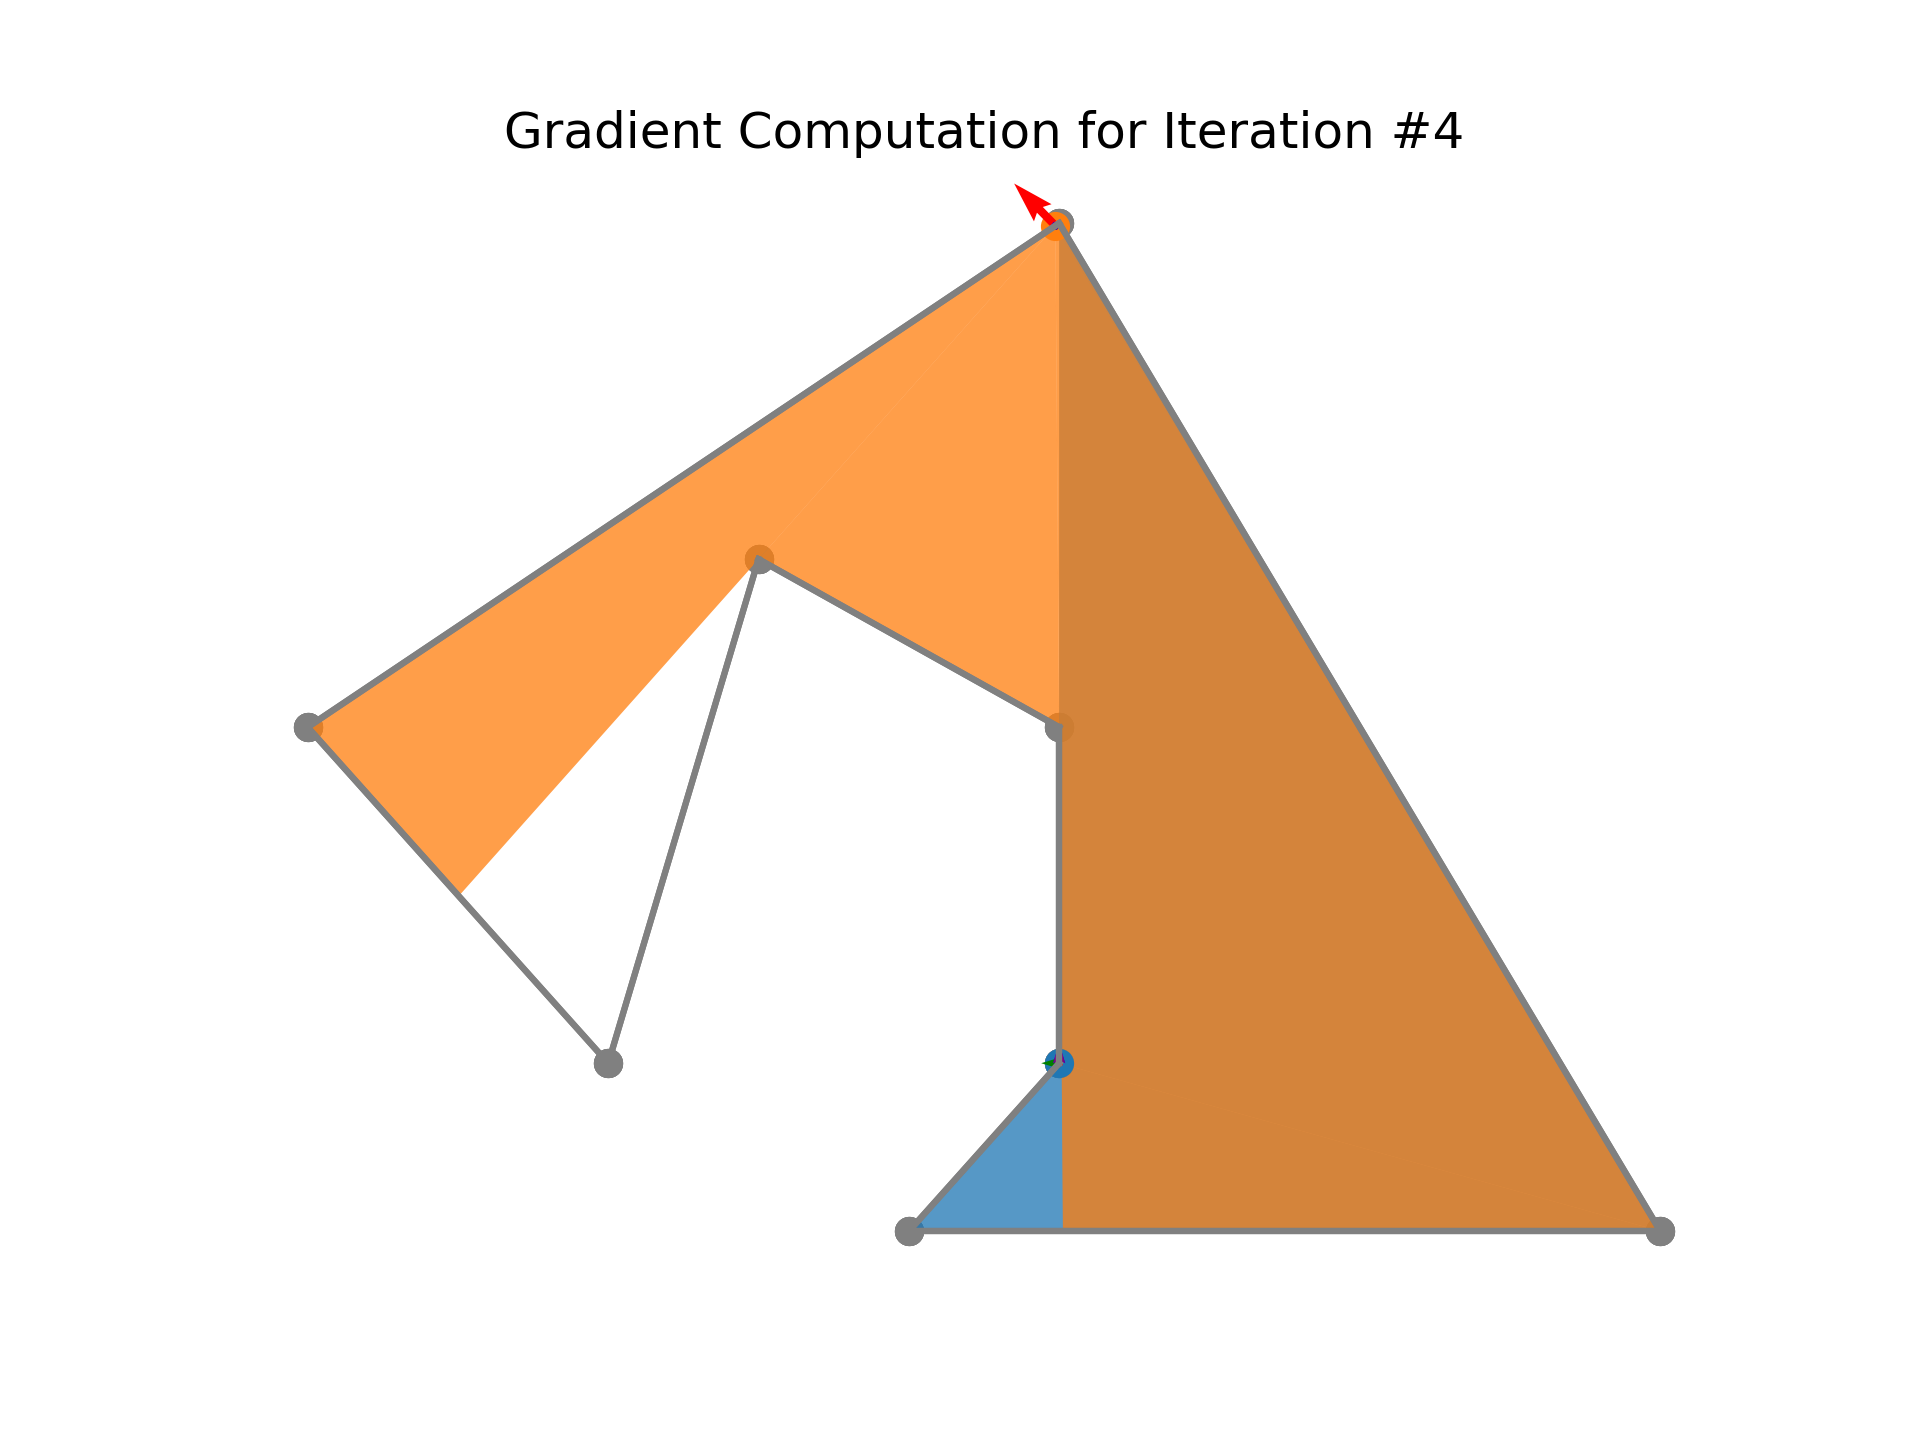
\includegraphics[width = \textwidth]{experiments/reflex_area_all_pos4.png}
            \caption{All heuristics. The blue guard is still on the reflex vertex (in the reflex area).}
        \end{subfigure}
        \hfill
        \begin{subfigure}{0.45\textwidth}
            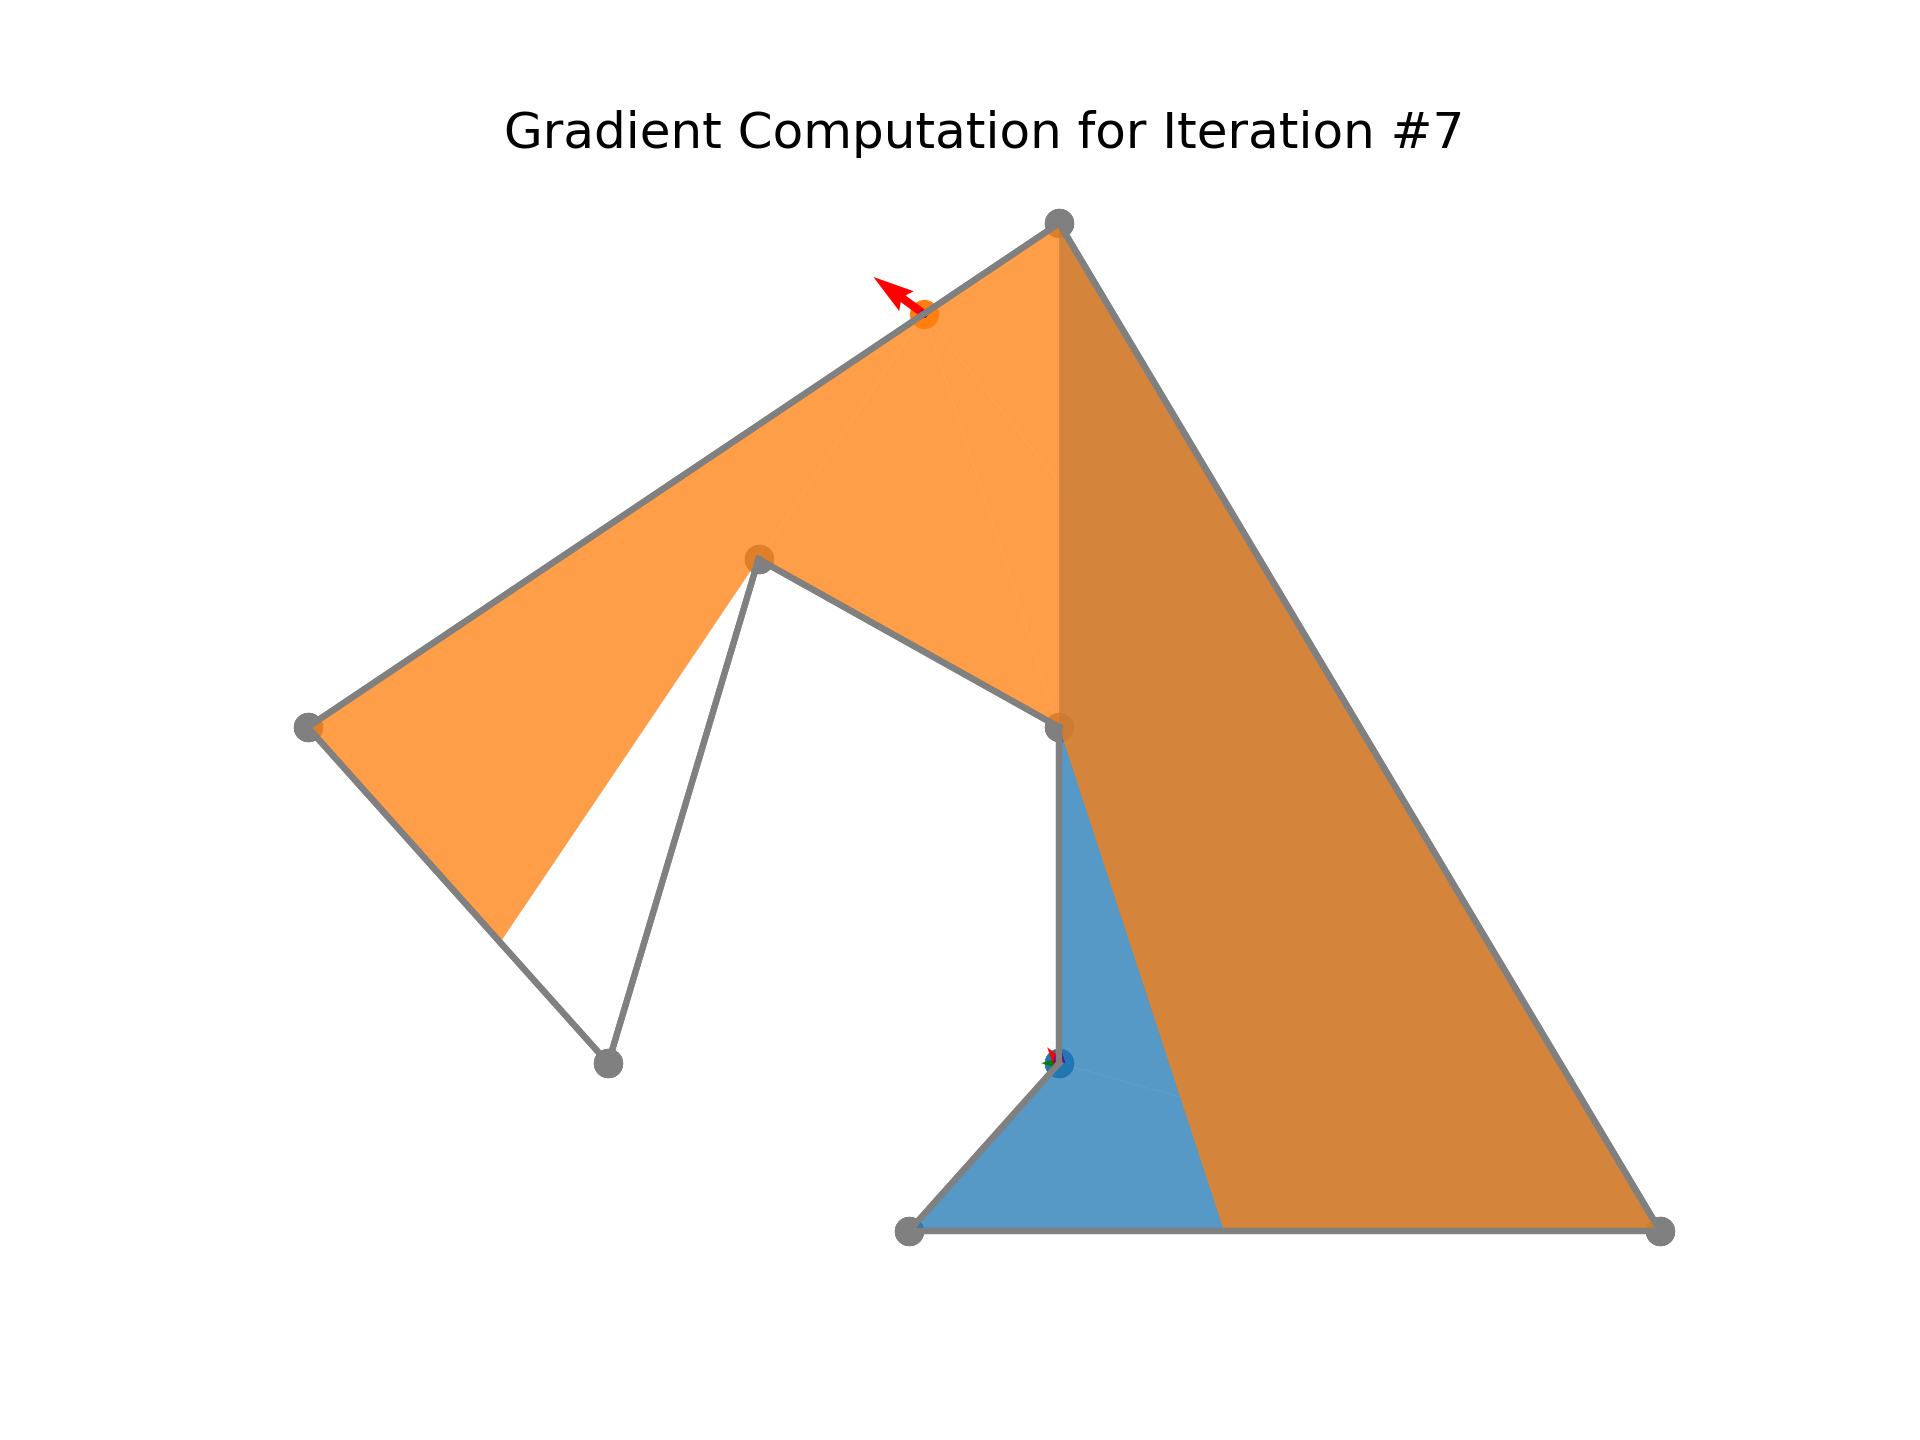
\includegraphics[width = \textwidth]{experiments/reflex_area_no_pos7.png}
            \caption{No reflex area. The blue guard is back on the reflex vertex.}
            \label{fig:reflex_area_no4}
        \end{subfigure}
        \caption{Comparison between using and not using the reflex area heuristic on an arbitrary polygon guarded by two guards.}
        \label{fig:reflex_area_eg}
    % \end{resizebox}
    \end{adjustbox}
    \end{figure}
\newpage



\begin{figure}[h!]
    \centering
    \begin{subfigure}{0.45\textwidth}
        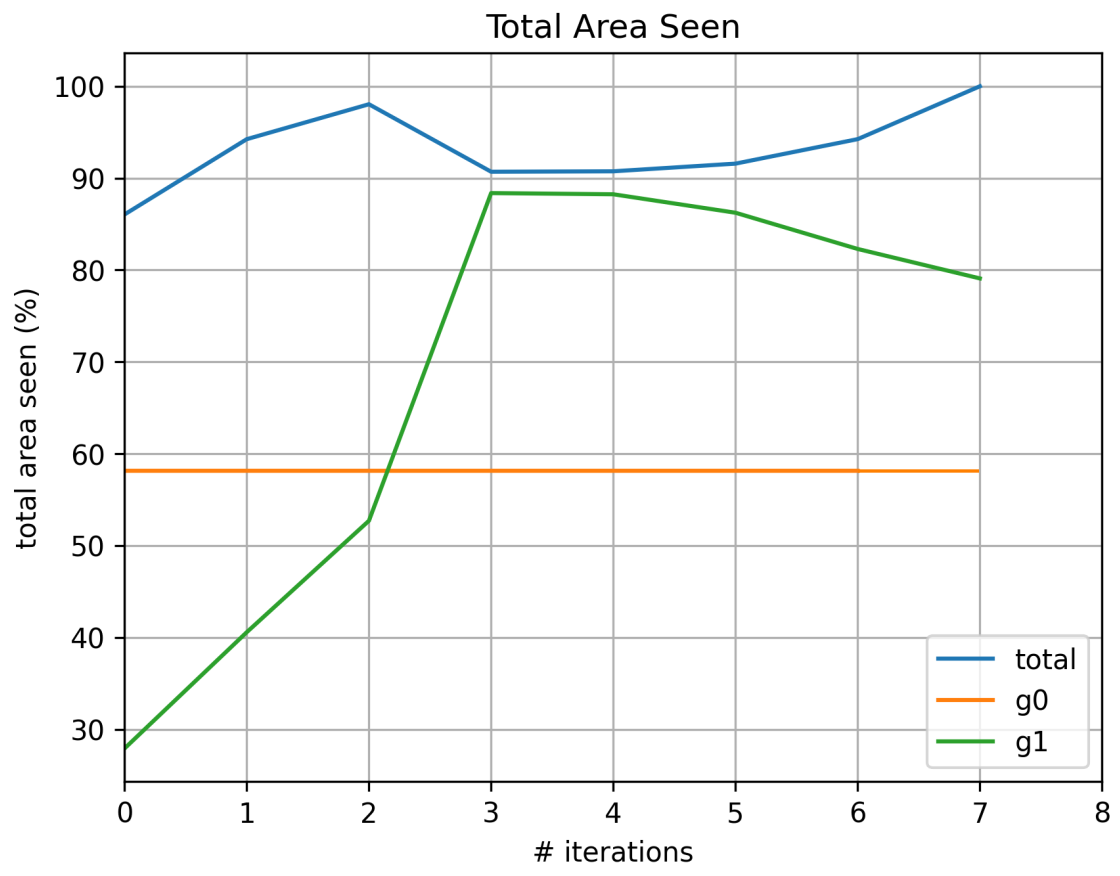
\includegraphics[width = \textwidth]{experiments/area_reflex_area_all2.png}
        \caption{Area seen for all heuristics on another arbitrary polygon.}
        \label{fig:area_reflex_area_all}
    \end{subfigure}
    \hfill
    \begin{subfigure}{0.45\textwidth}
        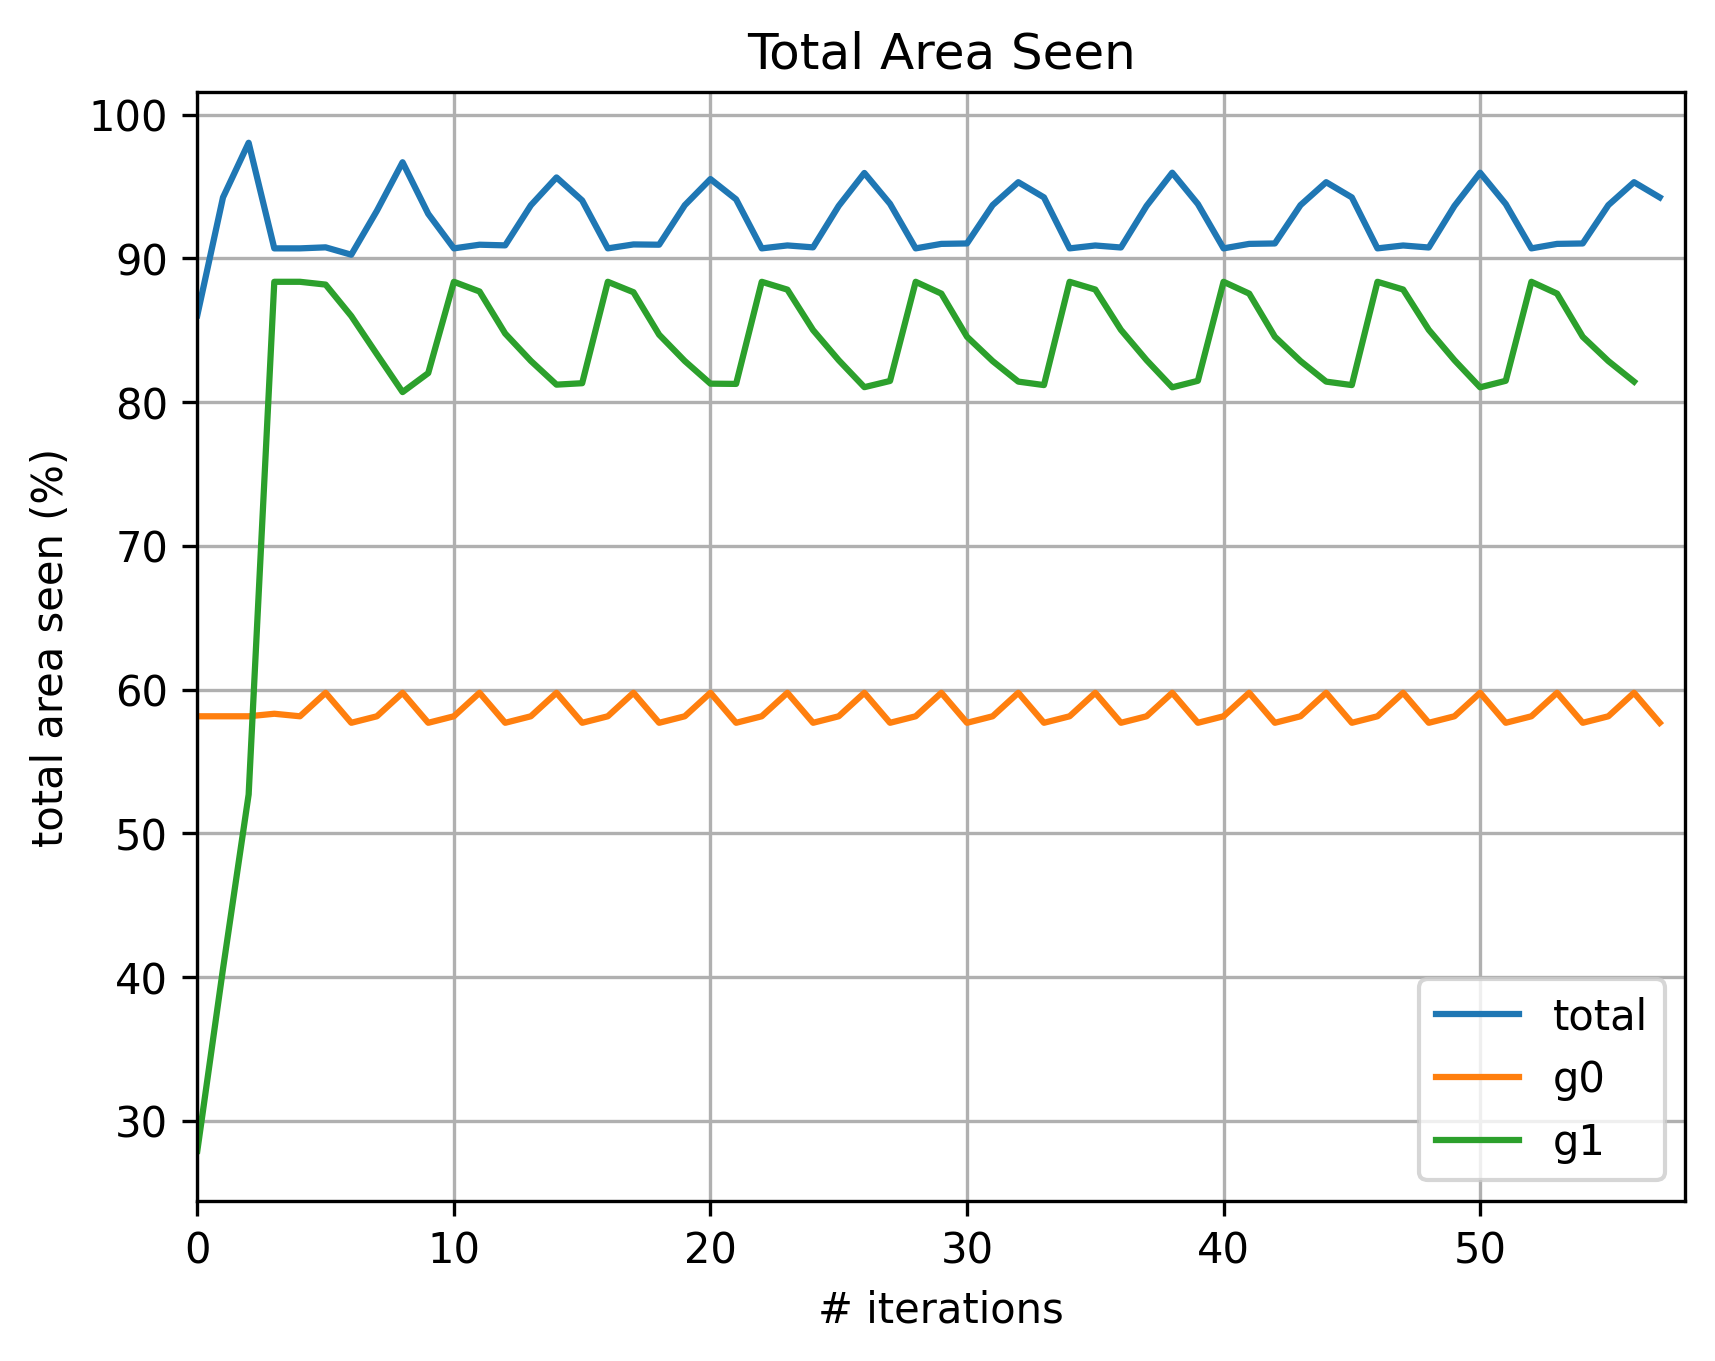
\includegraphics[width = \textwidth]{experiments/area_reflex_area_no.png}
        \caption{Area seen for no reflex area heuristic on another arbitrary polygon.}
        \label{fig:area_reflex_area_no}
    \end{subfigure}
    \caption{Area comparison between using and not using the reflex area heuristic on an arbitrary polygon guarded by two guards.}
    \label{fig:area_reflex_area}
\end{figure}



% \newpage
\subsubsection{Without Line Search}
In this section we  discuss the impact line search has on the overall behaviour of the algorithm. As introduced in Section \ref{sec:line_search}, line search determines how far a guard should move towards the direction movement vector. In this way, it computes the optimal position of a guard on the movement direction given a step size.

Line Search has step size $s$, maximum movement factor $x$ and starting factor $\frac{s^t}{x}, t = 0$ as hyperparameters. For our experiments, we choose $s = 2$ and $x = 32$. We start with a factor of $\frac 1 32$ for the movement vector. We  increase it by a step size of 2 up to factor 32.  In this way we generate 10 solutions in total, one for every step $\frac{1}{32}, \frac{1}{16}, \frac 1 8, ..., 1, 2, 4, ..., 32$. This  allows us to search a larger space of position possibilities knowing the direction of the movement vector. We  pick the best solution along all the step size based on the largest area increase. 

\begin{figure}[h!]
    \centering
    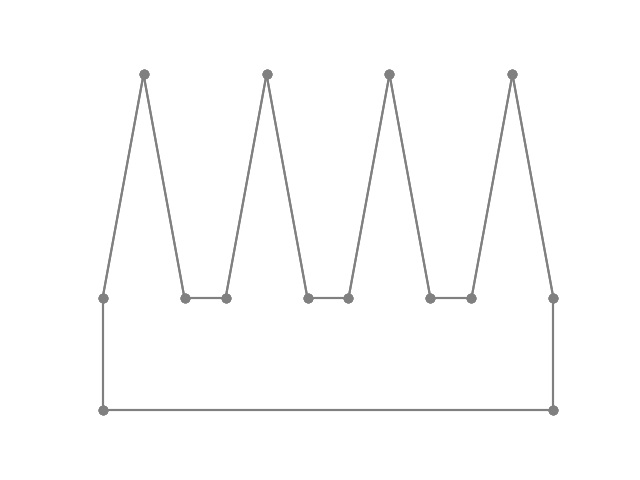
\includegraphics[width = 0.5\textwidth]{experiments/comb.png}
    \caption{Polygon in the shape of a comb with four teeth.}
    \label{fig:comb}
\end{figure}

A suggestive way to observe how well line search works is with the comb polygon with four teeth from Figure \ref{fig:comb}. Comb polygons with $t$ teeth require $t$ guards to be guarded, one guard for each tooth. This is because the space in between the teeth is large enough so that guards cannot fully see two teeth simultaneously. In our case, $t = 4$. We  compare how the guards move when we are using all the heuristics to when we are not using line search. They  start at the same fixed position in both cases, so we  focus on observing their movements.


Figure \ref{fig:no_line_search} displays the area seen per iteration for the comb polygon with four teeth. Both the total area seen and the individual area seen by each guard are shown. Starting with around 82.5\% total area seen, the global optimum is eventually found. Nonetheless, using line search clearly makes a difference between Subfigures \ref{fig:no_line_search1} and \ref{fig:no_line_search2}. The first noticeable difference is the number of iterations. Using line search allows the guards to find their optimal positions in 3 iterations, with a steady increase in the total area seen. Note that not all guards were moved in iteration 3. This is because the polygon was fully seen after moving only two of the guards. On the other hand, in subfigure \ref{fig:no_line_search2} not using line search results in the optimal position to be found in more than 80 iterations. Additionally, 3 of the guards found their optimal position after the $30^{\text{th}}$ iteration, whereas the last 50 iterations are spent on only one guard finding its own.


\begin{figure}[h!]
    \centering
    \begin{subfigure}{0.45\textwidth}
        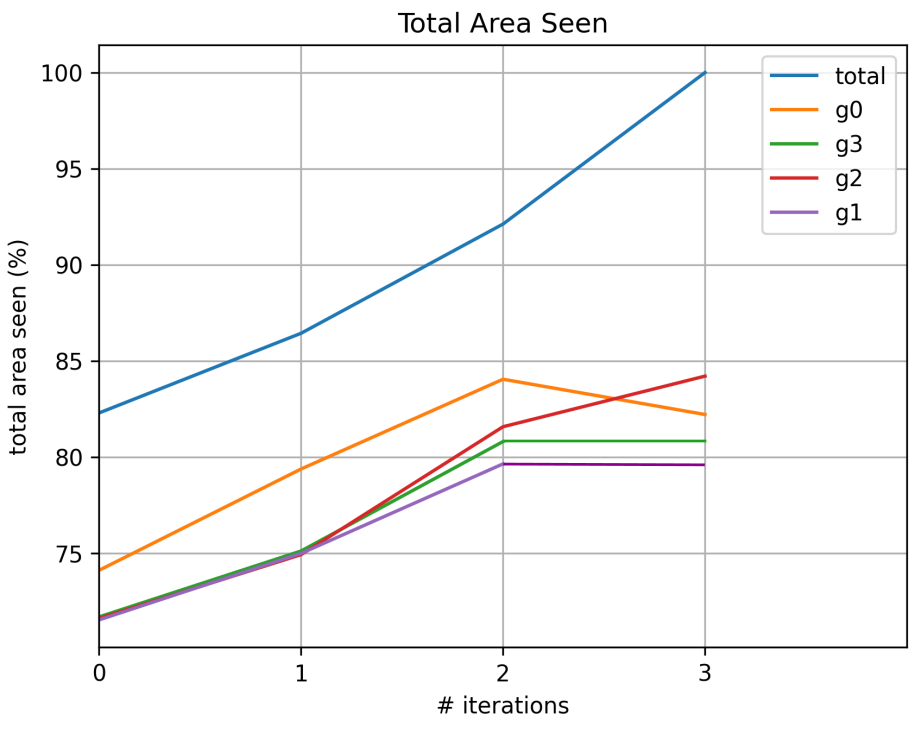
\includegraphics[width = \textwidth]{experiments/area_comb_easy_all2.png}
        \caption{All heuristics.}
        \label{fig:no_line_search1}
    \end{subfigure}
    \hfill
    \begin{subfigure}{0.45\textwidth}
        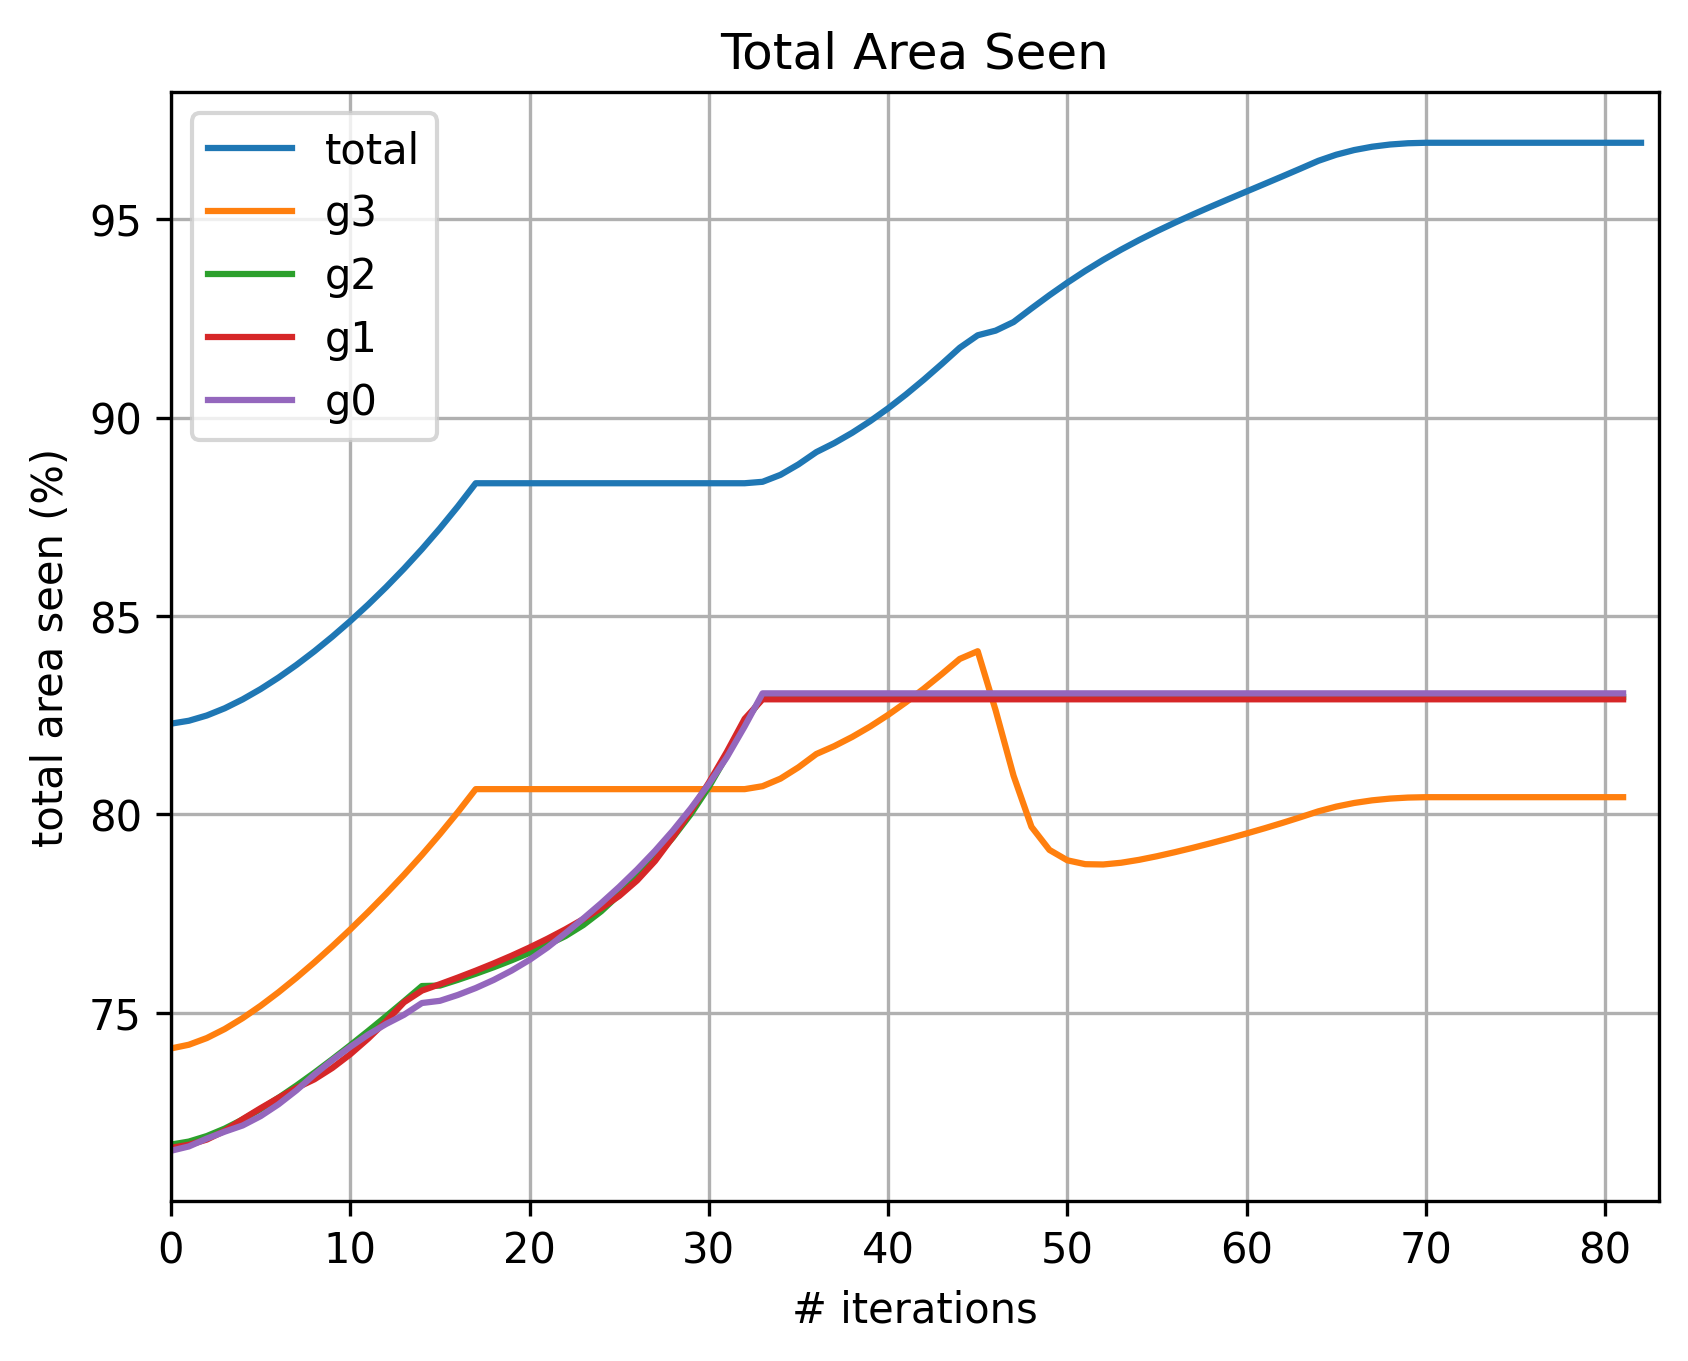
\includegraphics[width = \textwidth]{experiments/area_comb_no_linear_search.png}
        \caption{No line search.}
        \label{fig:no_line_search2}
    \end{subfigure}
    \caption{Total area seen per iteration for the comb polygon with four teeth, guarded by four guards.}
    \label{fig:no_line_search}
\end{figure}

Therefore, we reckon that line search significantly and more efficiently speeds up the process of finding the optimal position for each guard. In this way, each guard moves faster to its optimal position. The situation where multiple guards that have found their optimal position have to wait for only one guard to find its own is also avoided.

% \newpage
\subsubsection{Without Angle Behind Reflex Vertex}
In this section we  discuss the benefits of using the angle behind reflex vertices. Section \ref{sec:angle} introduced this heuristic. The idea behind this technique is that guards should be drawn faster to larger unseen areas behind reflex vertices. 
% Conversely, if the unseen area behind the reflex vertex is very small, we don't want guards to move towards it. 
In this way, we prioritise unseen areas based on their size, while still accounting for the small unseen areas.

We  compare how the guards move when we are using all the heuristics to when we are not taking into account the angle behind the reflex vertex. We  use an arbitrary polygon as an example, that needs three guards to be fully seen. Figure \ref{fig:no_angle_eg} shows a comparison between using and not using the angle behind the reflex vertex heuristic. Subfigures \ref{fig:all_angle_pos0} and \ref{fig:all_angle_pos1} display the first two iterations of the algorithm when all heuristics are used. Subfigures \ref{fig:no_angle_pos0} and \ref{fig:no_angle_pos1} focus on the first two iterations when not using the heuristic.

\newpage
We  observe a major difference in the way the final movement vector is computed for the orange guard in the two cases. When all heuristics are used, the movements of the guards are much smaller and smoother. For example, in Subfigure \ref{fig:no_angle_pos0}, the orange guard has a large movement vector outside the polygon due to the unseen part in the upper pocket. When we also take into account the angles behind the reflex vertices in the pocket, its movement vectors become much smaller (Subfigure \ref{fig:all_angle_pos0}). In fact, the orange guard is also drawn slightly to the right part of the polygon, as it has a larger angle behind the reflex vertex. That part of the polygon is already seen by the blue guard, so it starts moving towards the upper pocket in Subfigure \ref{fig:all_angle_pos1}.

\begin{figure}[h!]
    \centering
    \begin{subfigure}{0.45\textwidth}
        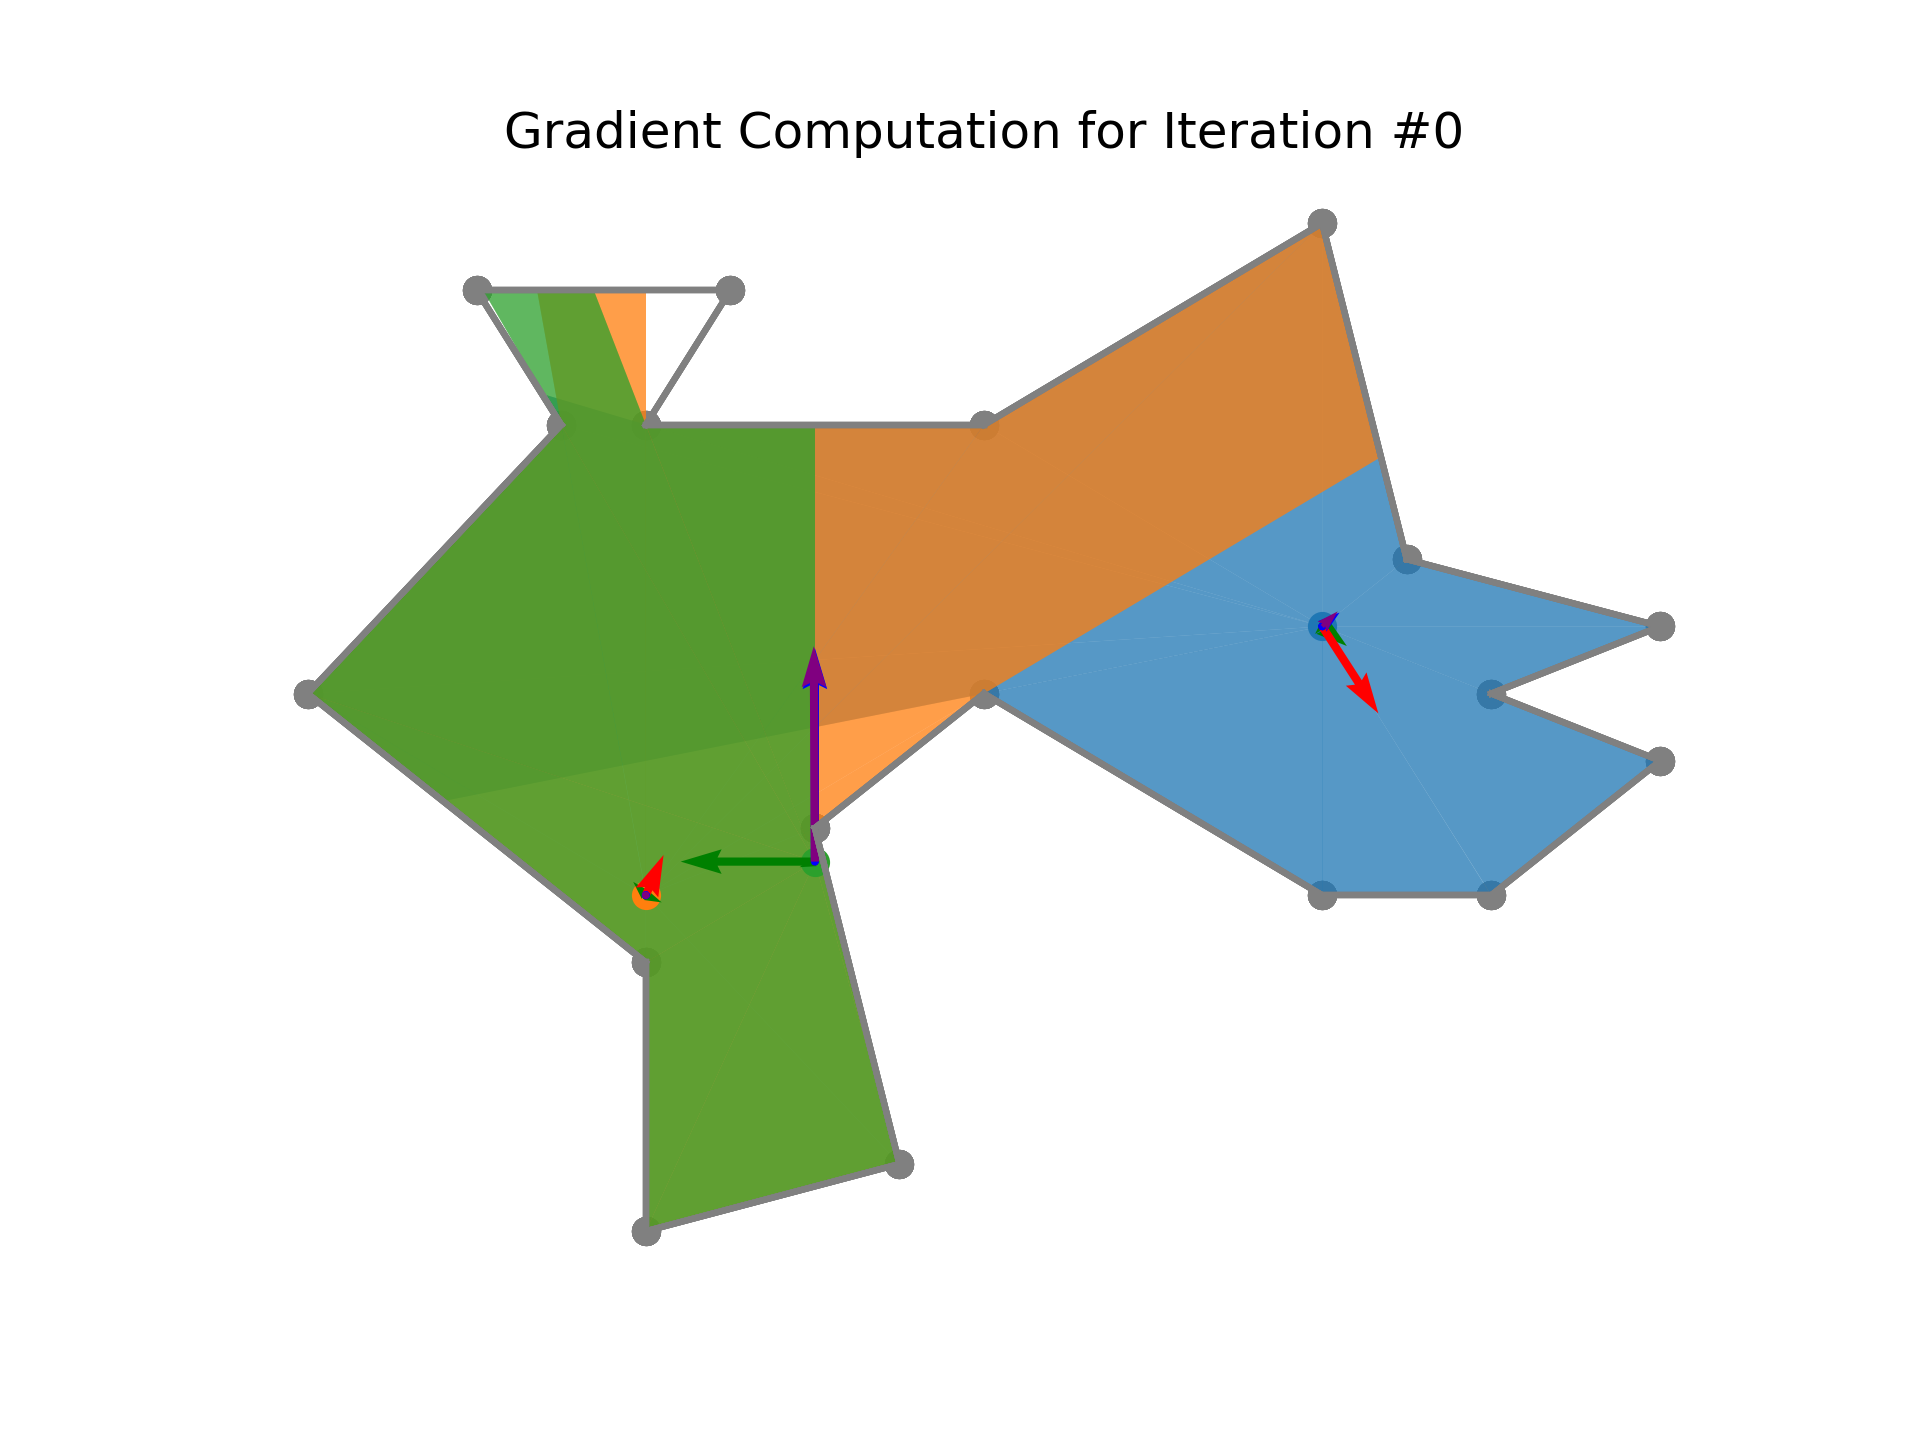
\includegraphics[width = \textwidth]{experiments/random_all_pull_pos0_fixed.png}
        \caption{All heuristics. The orange guard's movement is towards upper right.}
        \label{fig:all_angle_pos0}
    \end{subfigure}
    \hfill
    \begin{subfigure}{0.45\textwidth}
        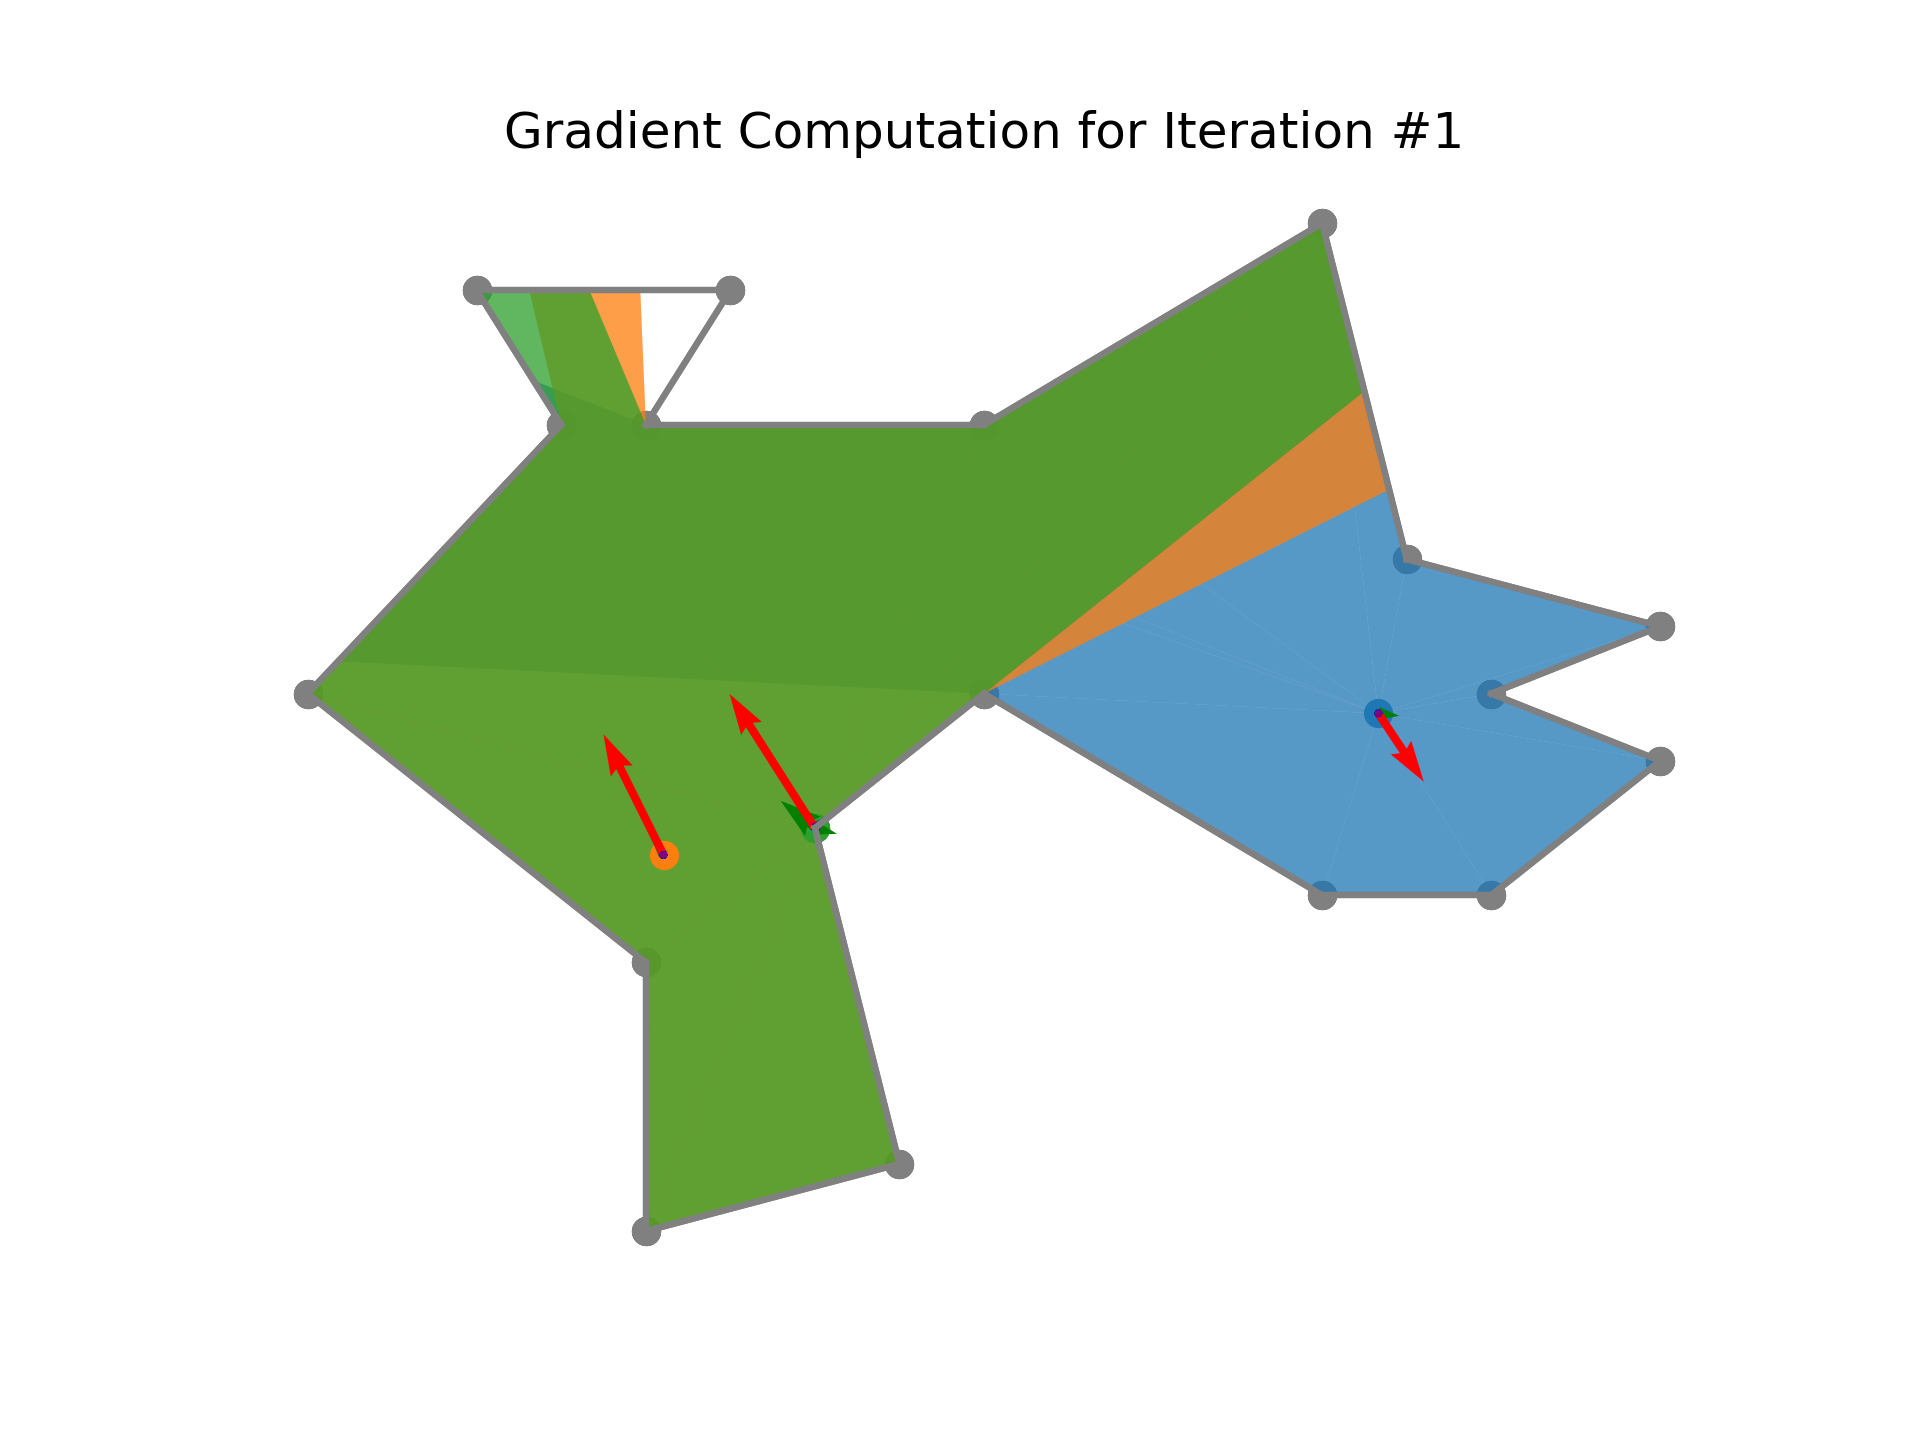
\includegraphics[width = \textwidth]{experiments/random_all_pull_pos1_fixed.png}
        \caption{All heuristics. The orange guard's movement is towards upper left.}
        \label{fig:all_angle_pos1}
    \end{subfigure}
    \vfill
    \begin{subfigure}{0.45\textwidth}
        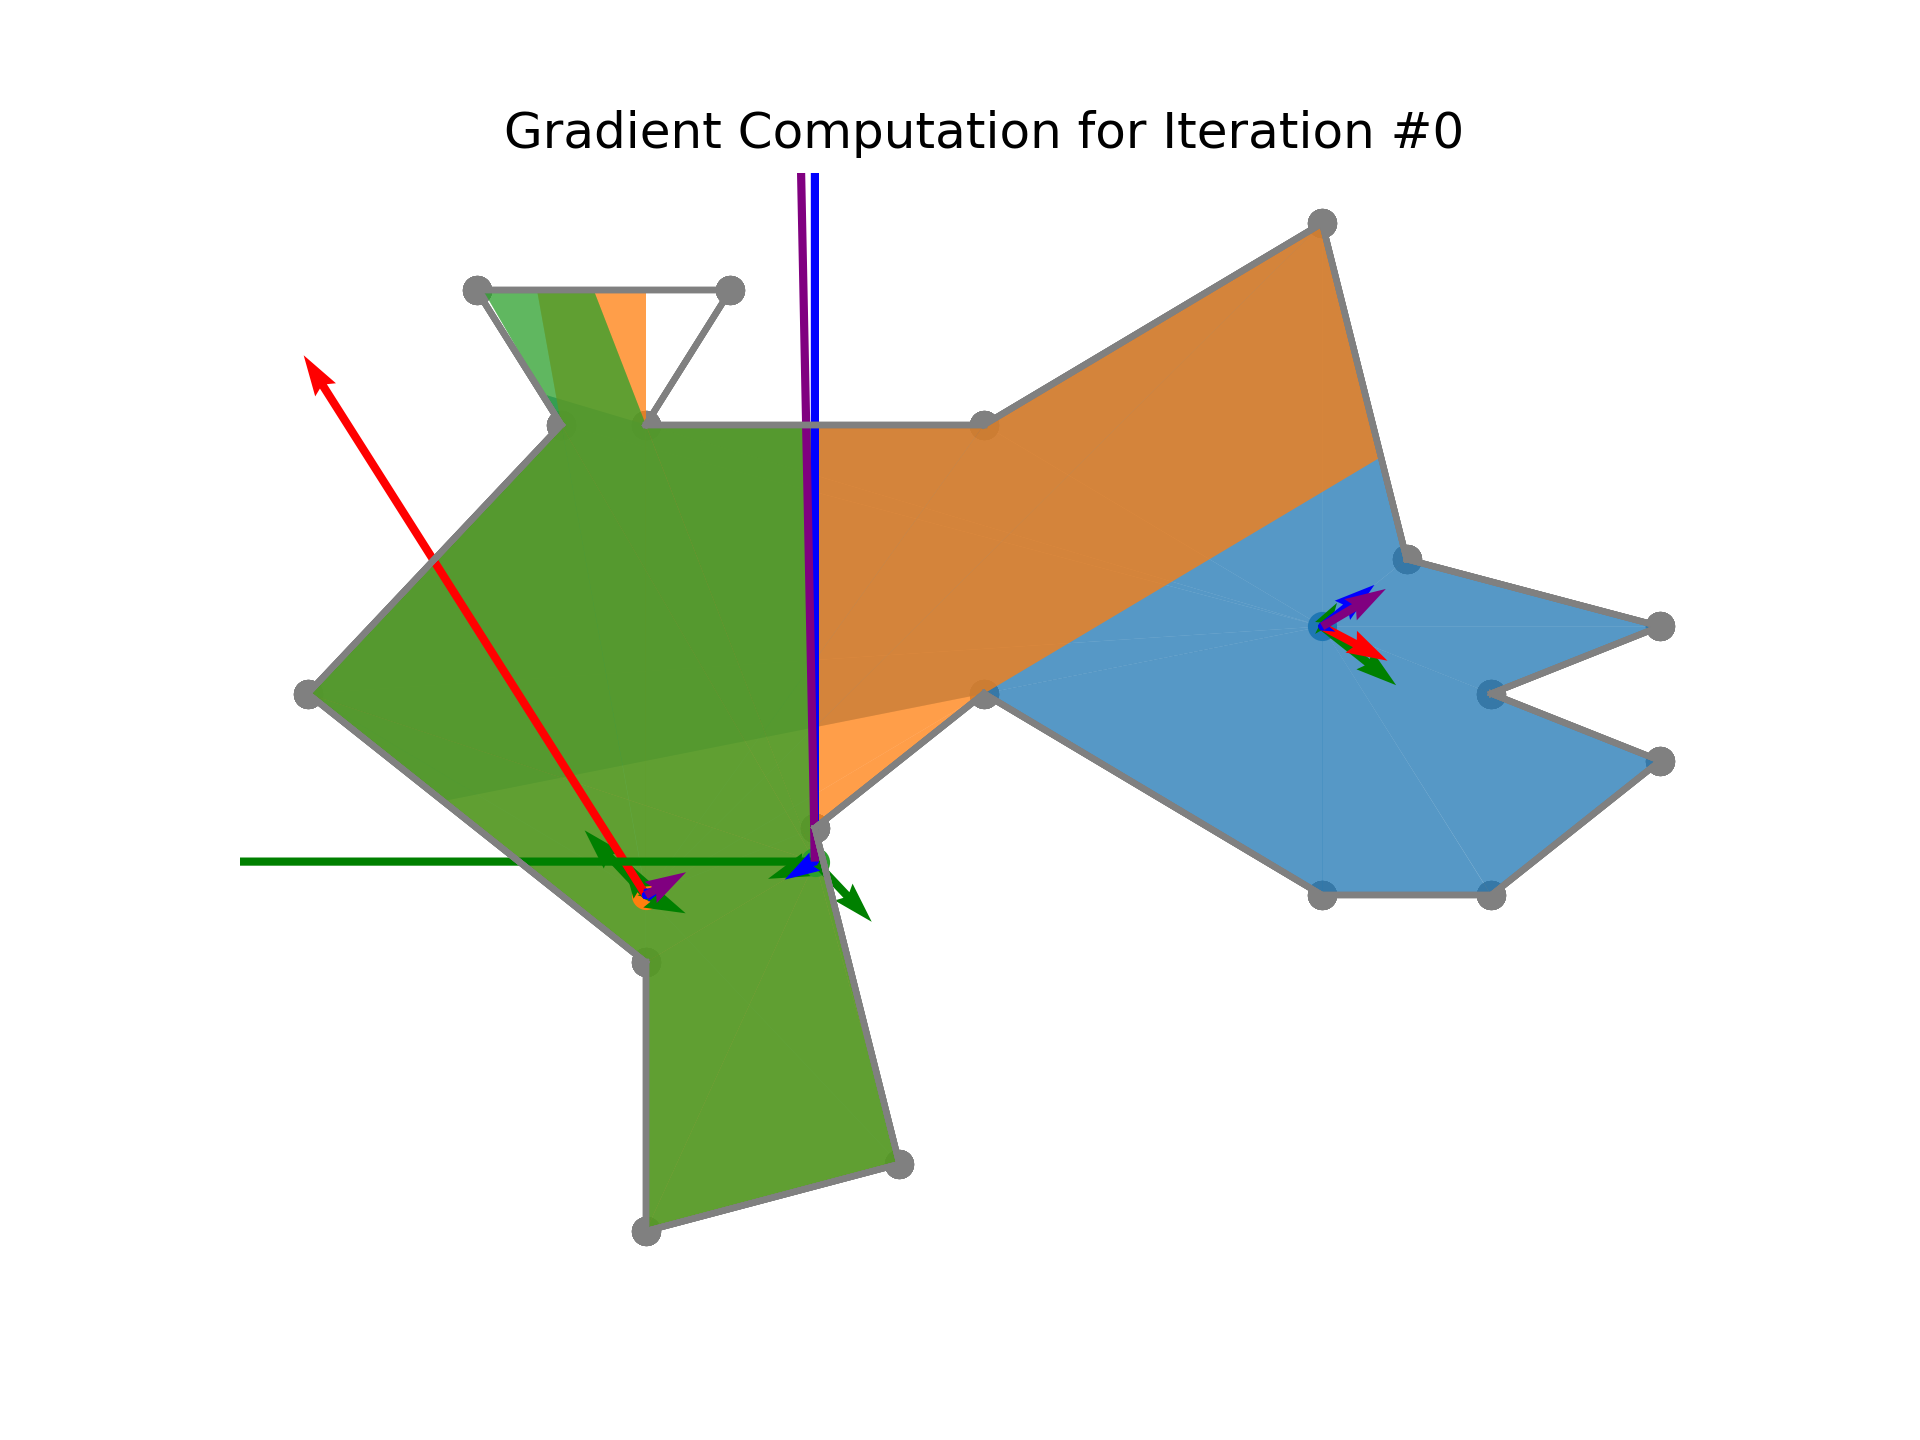
\includegraphics[width = \textwidth]{experiments/random_no_angle_pos0.png}
        \caption{No angle behind the reflex vertex. The orange guard's movement is all the way to the left boundary of the polygon.}
        \label{fig:no_angle_pos0}
    \end{subfigure}
    \hfill
    \begin{subfigure}{0.45\textwidth}
        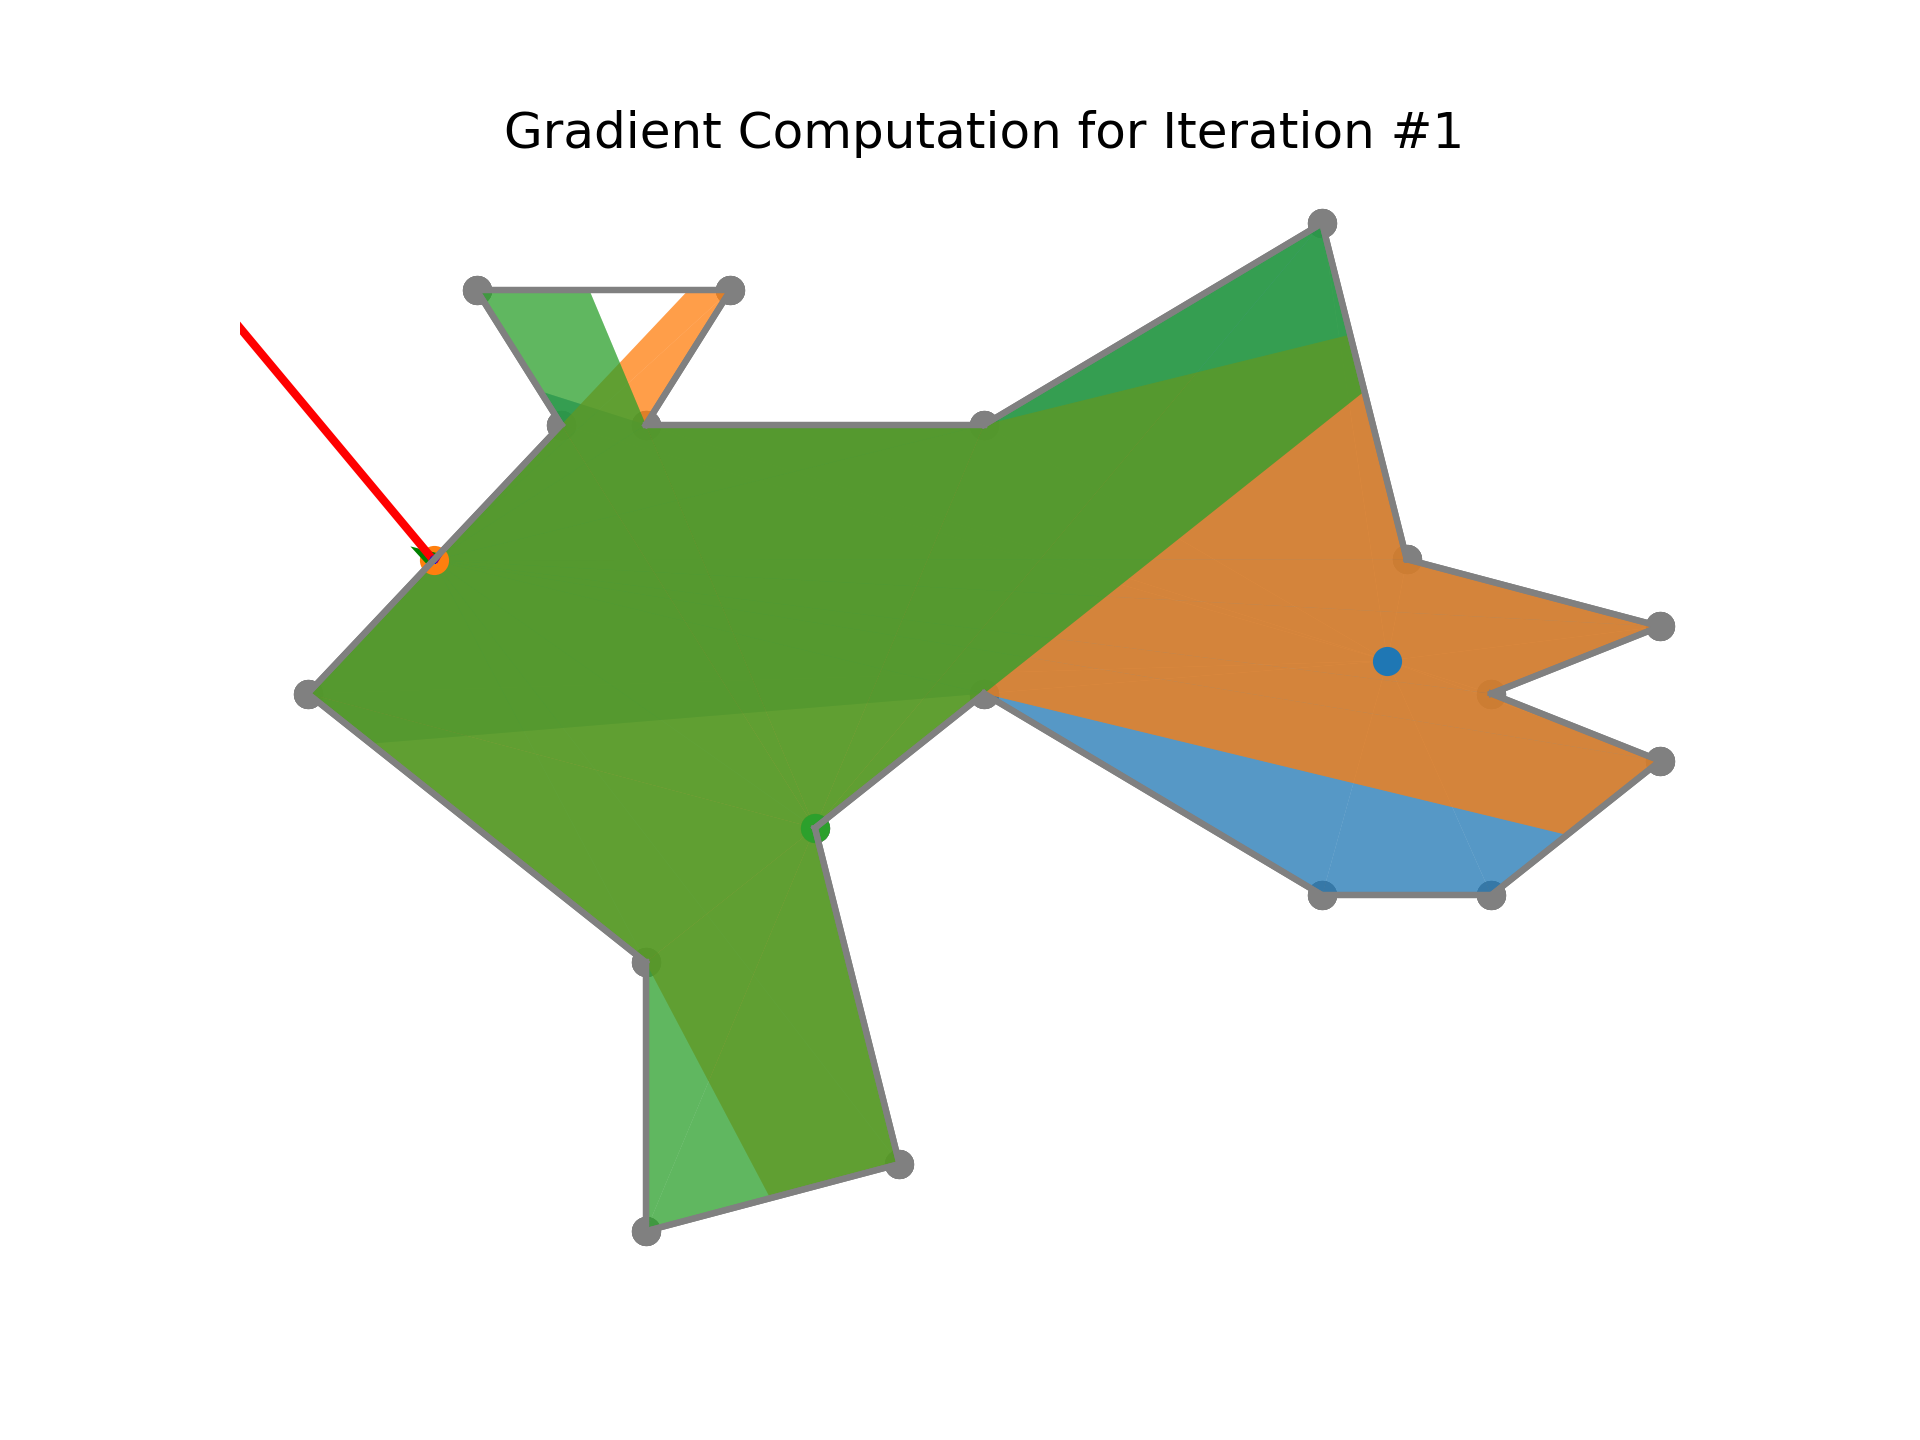
\includegraphics[width = \textwidth]{experiments/random_no_angle_pos1.png}
        \caption{No angle behind the reflex vertex. The orange guard's movement is towards the left-side outside the polygon.}
        \label{fig:no_angle_pos1}
    \end{subfigure}
    \caption{Example of different movements of guards with and without the angle behind the reflex vertex in an arbitrarily shaped polygon guarded by three guards. The total gradient vector is displayed in red, partial gradient vectors are green and the pull vector is purple.}
    \label{fig:no_angle_eg}
\end{figure}

In terms of efficiency, the optimal solution is achieved in more iterations when the angle heuristic is used. This is observed in Figure \ref{fig:no_angle_plots}. When using all heuristics, the optimal solution is achieved in 5 iterations (Subfigure \ref{fig:area_all_angle}). The movement of the guards is smooth. Two of the guards have an increasing seen area, whereas the orange guard moves slowly towards the upper pocket of the polygon. Not using the angle heuristic allows us to achieve the same goal in only 3 iterations, in a less smooth manner (Subfigure \ref{fig:area_no_angle}).

\begin{figure}[h!]
    \begin{subfigure}{0.45\textwidth}
        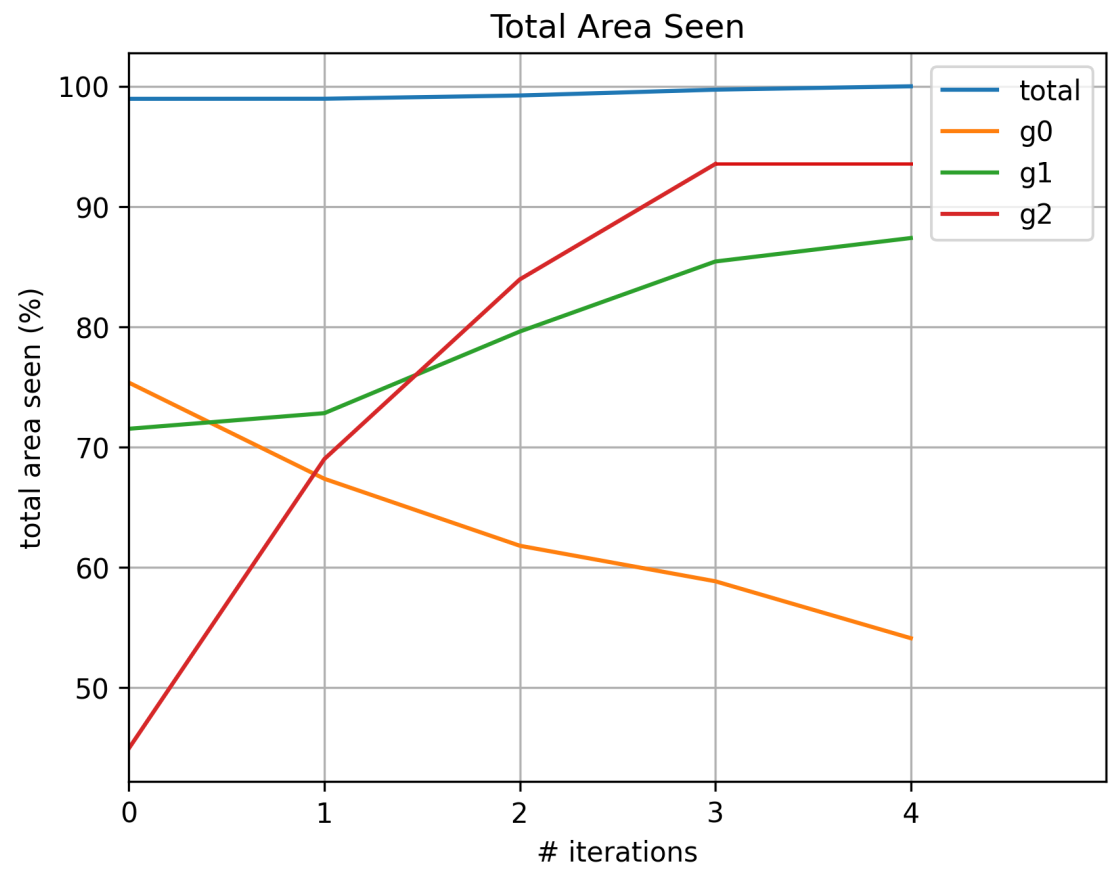
\includegraphics[width = \textwidth]{experiments/area_random_all_fixed2.png}
        \caption{Seen area for all heuristics.}
        \label{fig:area_all_angle}
    \end{subfigure}
    \hfill
    \begin{subfigure}{0.45\textwidth}
        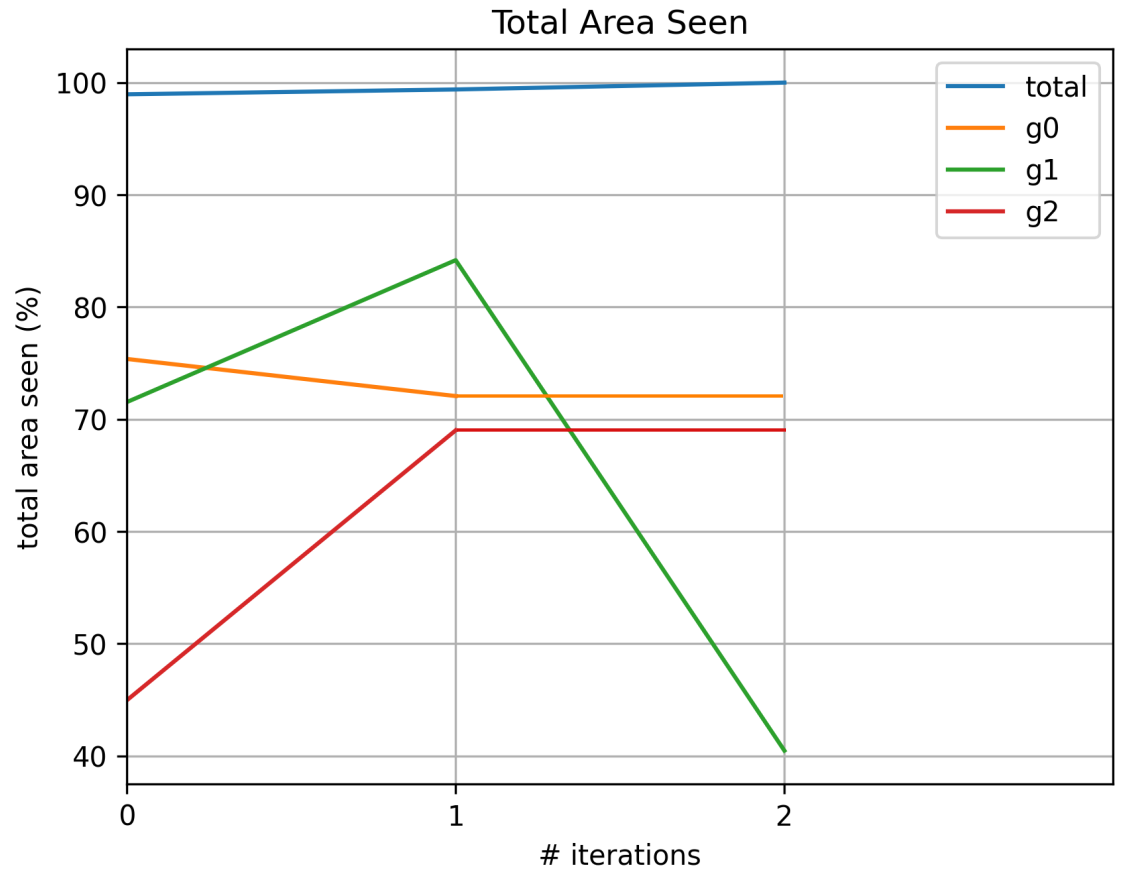
\includegraphics[width = \textwidth]{experiments/area_random_no_angle2.png}
        \caption{Seen area without the angle behind the reflex vertices.}
        \label{fig:area_no_angle}
    \end{subfigure}
    \caption{Total and individual areas seen per iteration for an arbitrarily shaped polygon guarded by three guards.}
    \label{fig:no_angle_plots}
\end{figure}

% \newpage
Therefore, computing the angle behind the reflex vertex is a heuristic that allows us to fine-tune and smoothen the movement of the guards. In this way, we  focus on moving fast towards the bigger unseen areas, while not neglecting the smaller ones. We could say that this heuristic offers a trade-off between the number of iterations and path smoothness. For this reason, the performance of the algorithm is influenced by the type of polygons it is applied to: polygons with sharper, narrower turns could benefit the most from this heuristic.


\subsubsection{No Hidden Movement}
In this section we  discuss the importance of using the hidden movement heuristic. Section \ref{sec:hidden_gradient} introduced it. The idea is based on the fact that we want guards to make progress, no matter how little. If a guard's visibility region is already seen by other guards (so its movement vector is zero), it is still unlikely that its position is optimal. Thus, we want the guard to still progress.

We  compare how the guards move when we are using all the heuristics to when we are not using the hidden movement heuristic. We  use the comb polygon with four teeth as an example. 

Figure \ref{fig:area_no_hidden_gradient} displays a comparison between using and not using the hidden movement in our algorithm. In Subfigure \ref{fig:area_comb_no_hidden_gradient} we  notice that the execution of the algorithm takes twice as many iterations than in Subfigure \ref{fig:area_comb_all2}. The reason behind this is the fact that for half of the iterations two of the guards do not move when no hidden gradient is used. Additionally, the total area seen in that case fluctuates. This is in contrast with the case where the hidden gradient heuristic is used. In that case, the total area seen is continuously increasing, and all guards who can make progress move.

\begin{figure}[h!]
    \centering
    \begin{subfigure}{0.45\textwidth}
        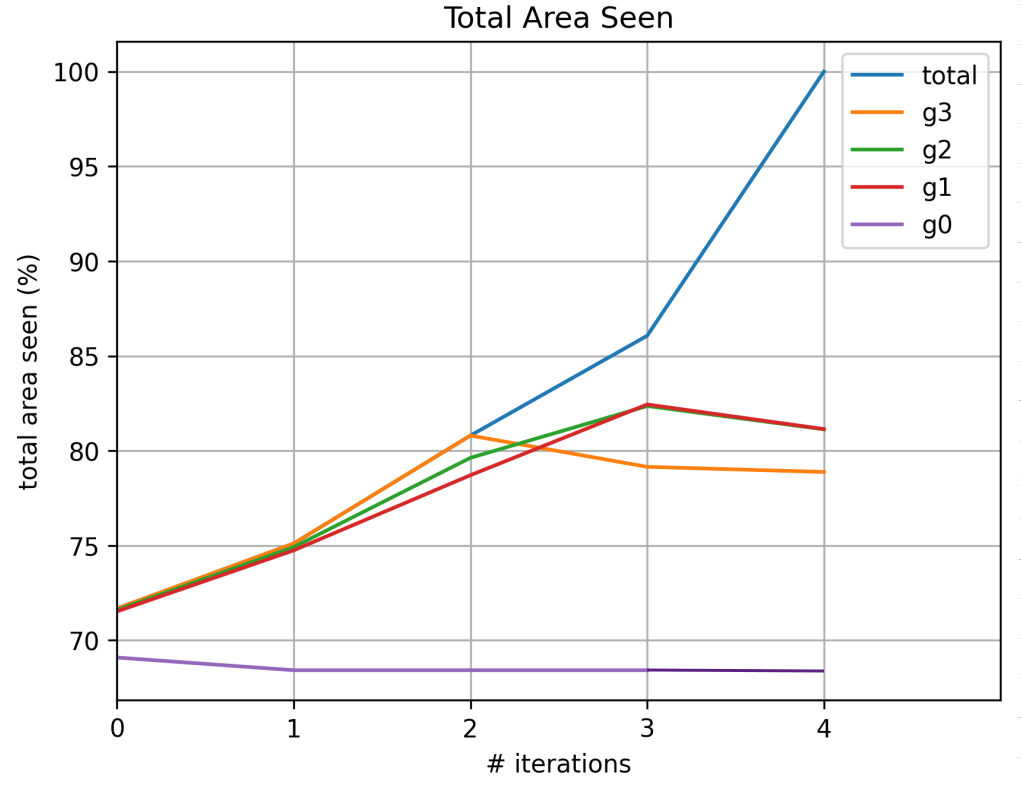
\includegraphics[width = \textwidth]{experiments/area_comb_all2.png}
        \caption{All heuristics.}
        \label{fig:area_comb_all2}
    \end{subfigure}
    \hfill
    \begin{subfigure}{0.45\textwidth}
        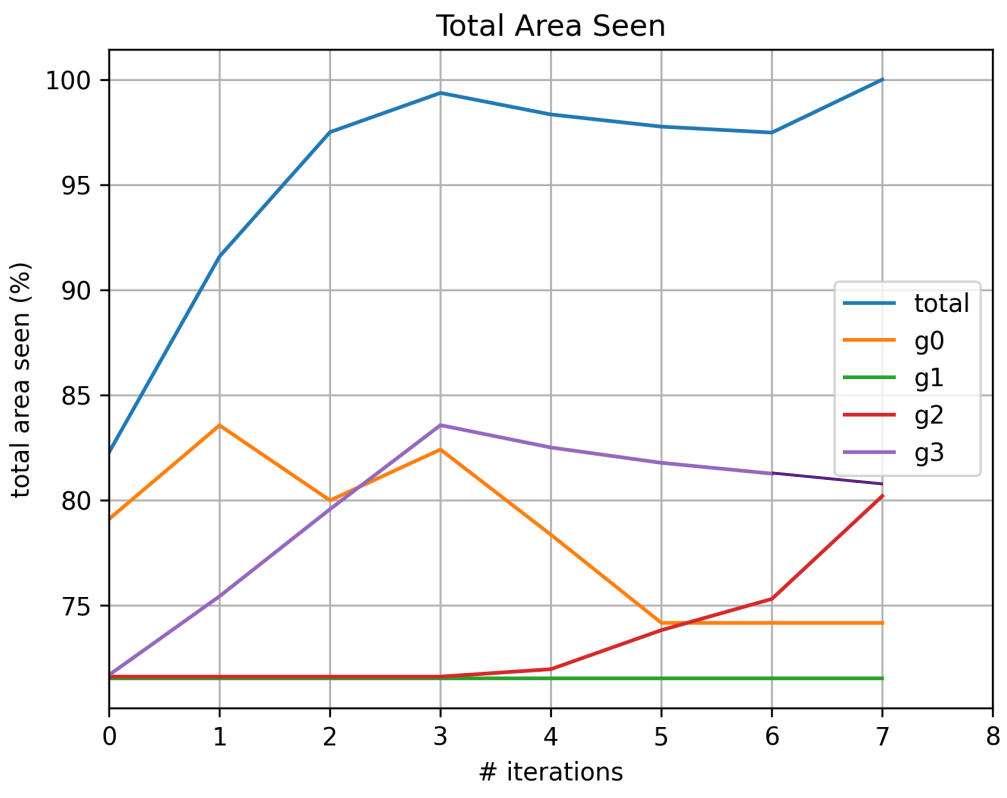
\includegraphics[width = \textwidth]{experiments/area_comb_no_hidden_gradient2.png}
        \caption{No hidden gradient.}
        \label{fig:area_comb_no_hidden_gradient}
    \end{subfigure}
    \caption{Seen area for the comb polygon with four teeth guarded by four guards.}
    \label{fig:area_no_hidden_gradient}
\end{figure}

Therefore, we reckon that the hidden gradient heuristic results in a significant improvement to our algorithm in terms of efficiency. In this way, all guards are ensured to make some progress towards their optimum and are not stalled.

\newpage
\subsubsection{Greedy Initialisation}
In this section we  discuss the benefits of using a greedy initialisation technique for our algorithm. Section \ref{sec:greedy} introduces it as beneficial for giving a head start to our algorithm. In our experiments we  greedily initialise the guards in the middle of the leftmost segment of each of their visibility regions. The reason behind this choice is that CGAL did not offer a quick way to pick a randomised position inside the visibility area. Due to the time constraints of this thesis, we decided to use a deterministic positioning.

So far we have not used greedy initialisation in any of our examples. The reason is that this technique already solves some polygons at guard placement time. An example in this case is the comb polygon with four teeth in Figure \ref{fig:comb_greedy}.

\begin{figure}[h!]
    \centering
    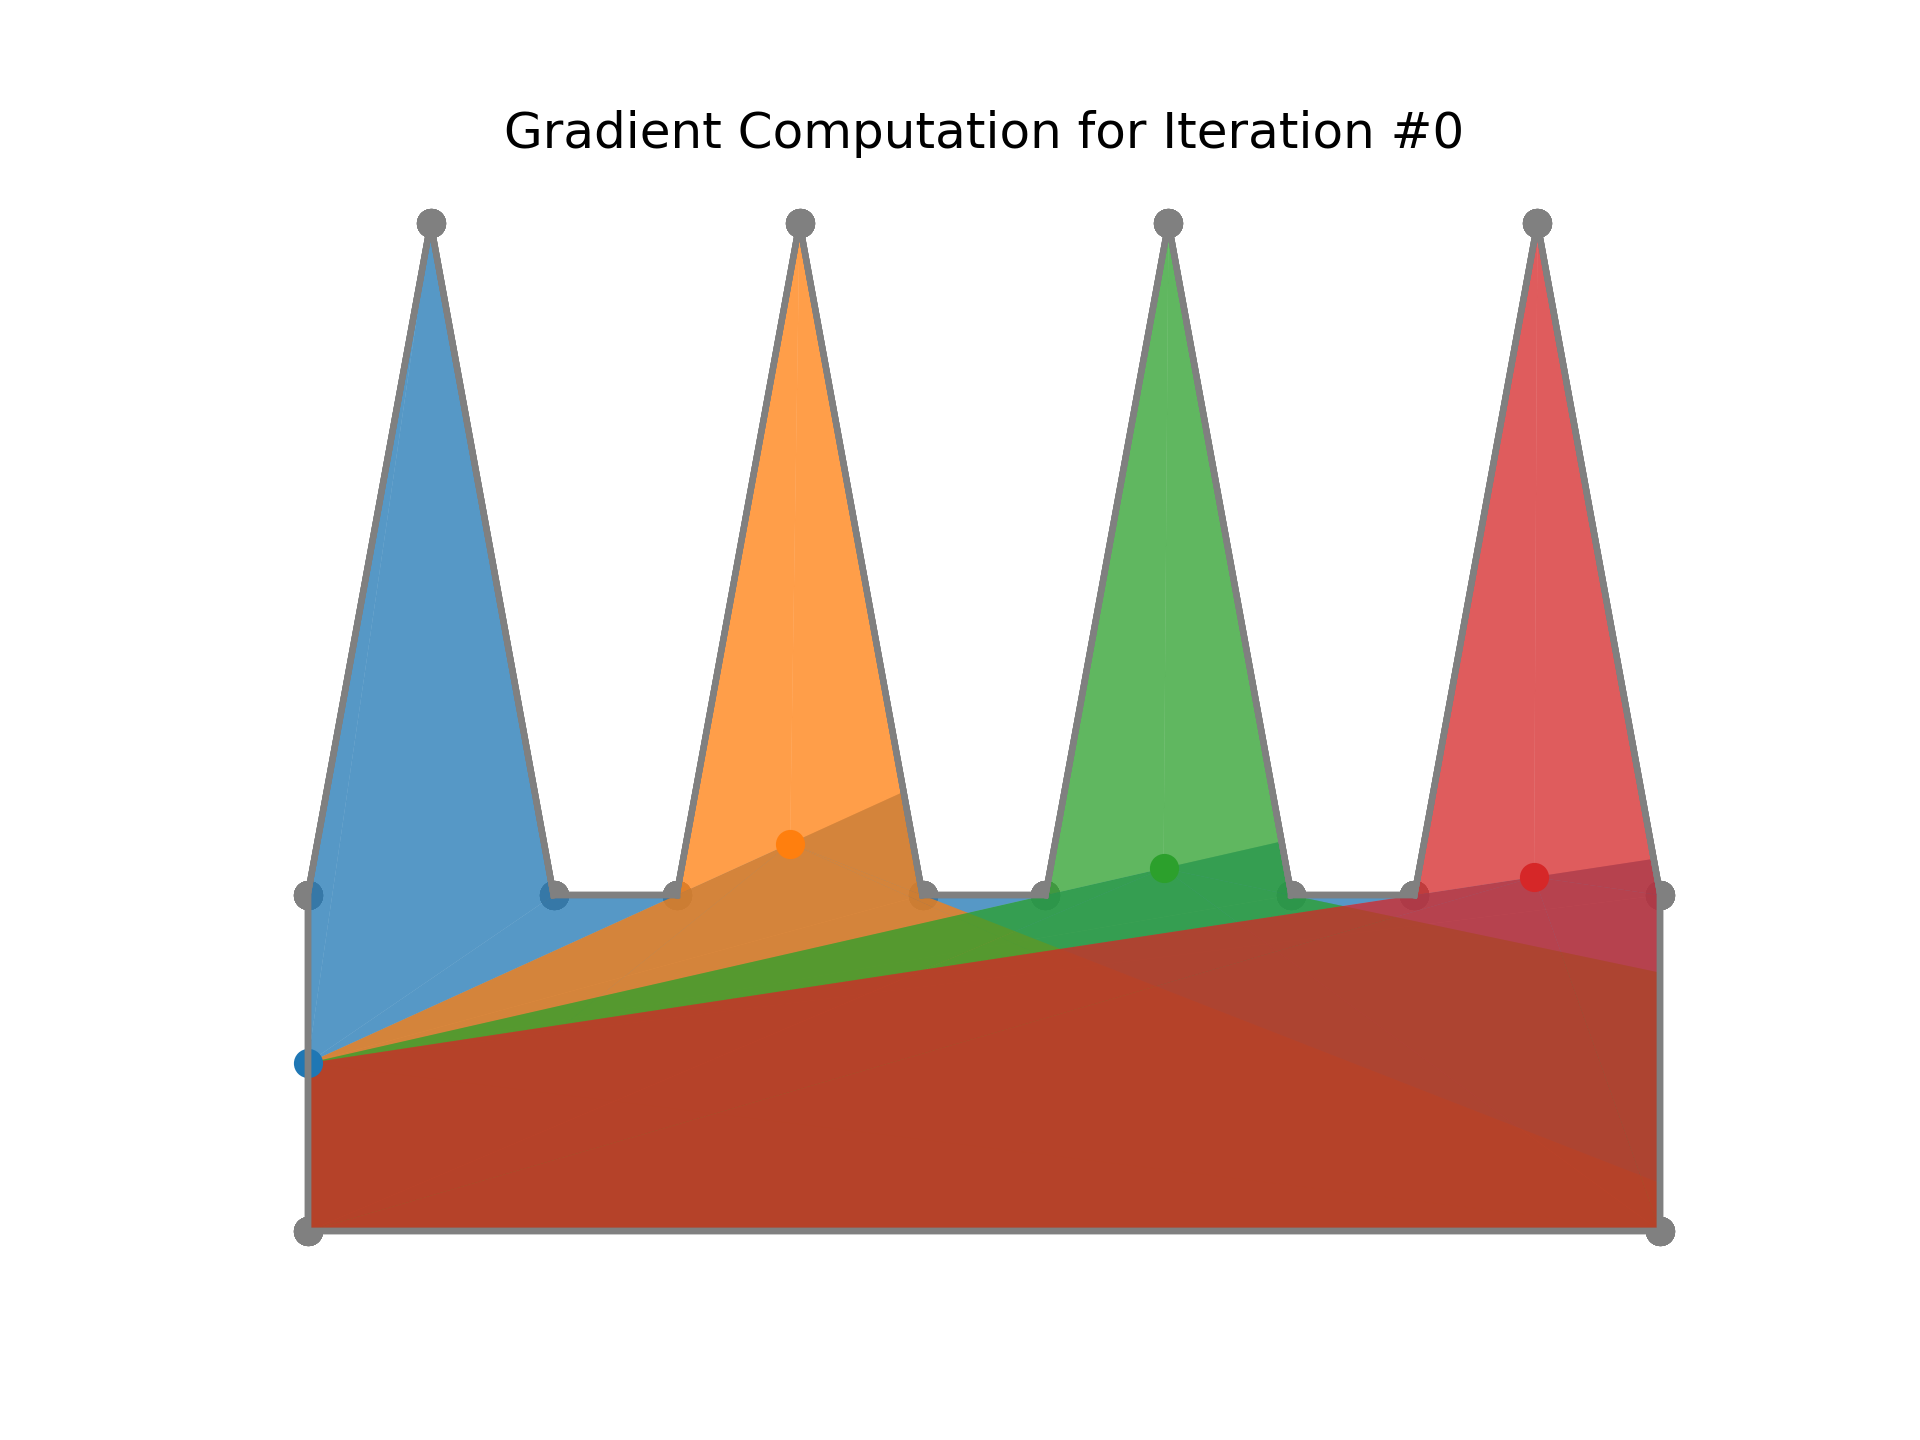
\includegraphics[width = 0.7\textwidth]{experiments/comb_greedy.png}
    \caption{The comb polygon with four teeth is already completely seen at greedy initialisation time.}
    \label{fig:comb_greedy}
\end{figure}

\newpage
In the case of polygons who are not completely seen at initialisation time, it is unclear whether the greedy placement improves the overall progress. How well the algorithm behaves is highly dependent on the initial placement of the guards. Namely, the algorithm often does not finish with different starting positions (it is stuck in local optima). Because of this drawback, we cannot create extensive experiments with different starting guard positions. 
% It is additionally not feasible to find a generalisation in the type of placements that allow the algorithm to finish.

Therefore, we believe that the greedy initialisation technique would benefit most from a deterministic placement if it were tailored to the shape of the polygon. Otherwise, an arbitrary placement would be most suitable for general cases. However, due to time constraints, this heuristic's performance is limited. So, it is to be explored with a more robust implementation that places guards arbitrarily.
% - momentum
% - reflex vertex pull
    % - onto reflex vertex
    % - pull Capping
% - line search
% - reflex area
% - hidden gradient
% - angle behind reflex vertex
% - greedy initialisation

% \newpage
\subsection{Scaling for the Comb Polygon}
In this section we  observe how the algorithm scales on the comb polygon. We  take the comb polygons with 2, 3, ..., 10, 15, 20, 50, 100 teeth. We  note how the algorithm progresses in terms of the total area seen per iteration.
As such, we  run the algorithm with all heuristics (but greedy initialisation) for all the mentioned comb polygons. All guards  start at the same $y$-coordinate, 0.1 units apart from each other. An example of such a starting point is found in Figure \ref{fig:comb6_start_pos}. In this way, we  ensure that the performance of the algorithm can be compared using the same starting position of the guards. We  deem a timeout of one hour for declaring an algorithm infeasible for larger polygons. We  then analyse how the algorithm performed under each of the circumstances. Lastly, we  offer some points of improvement.

\begin{figure}[h!]
    \centering
    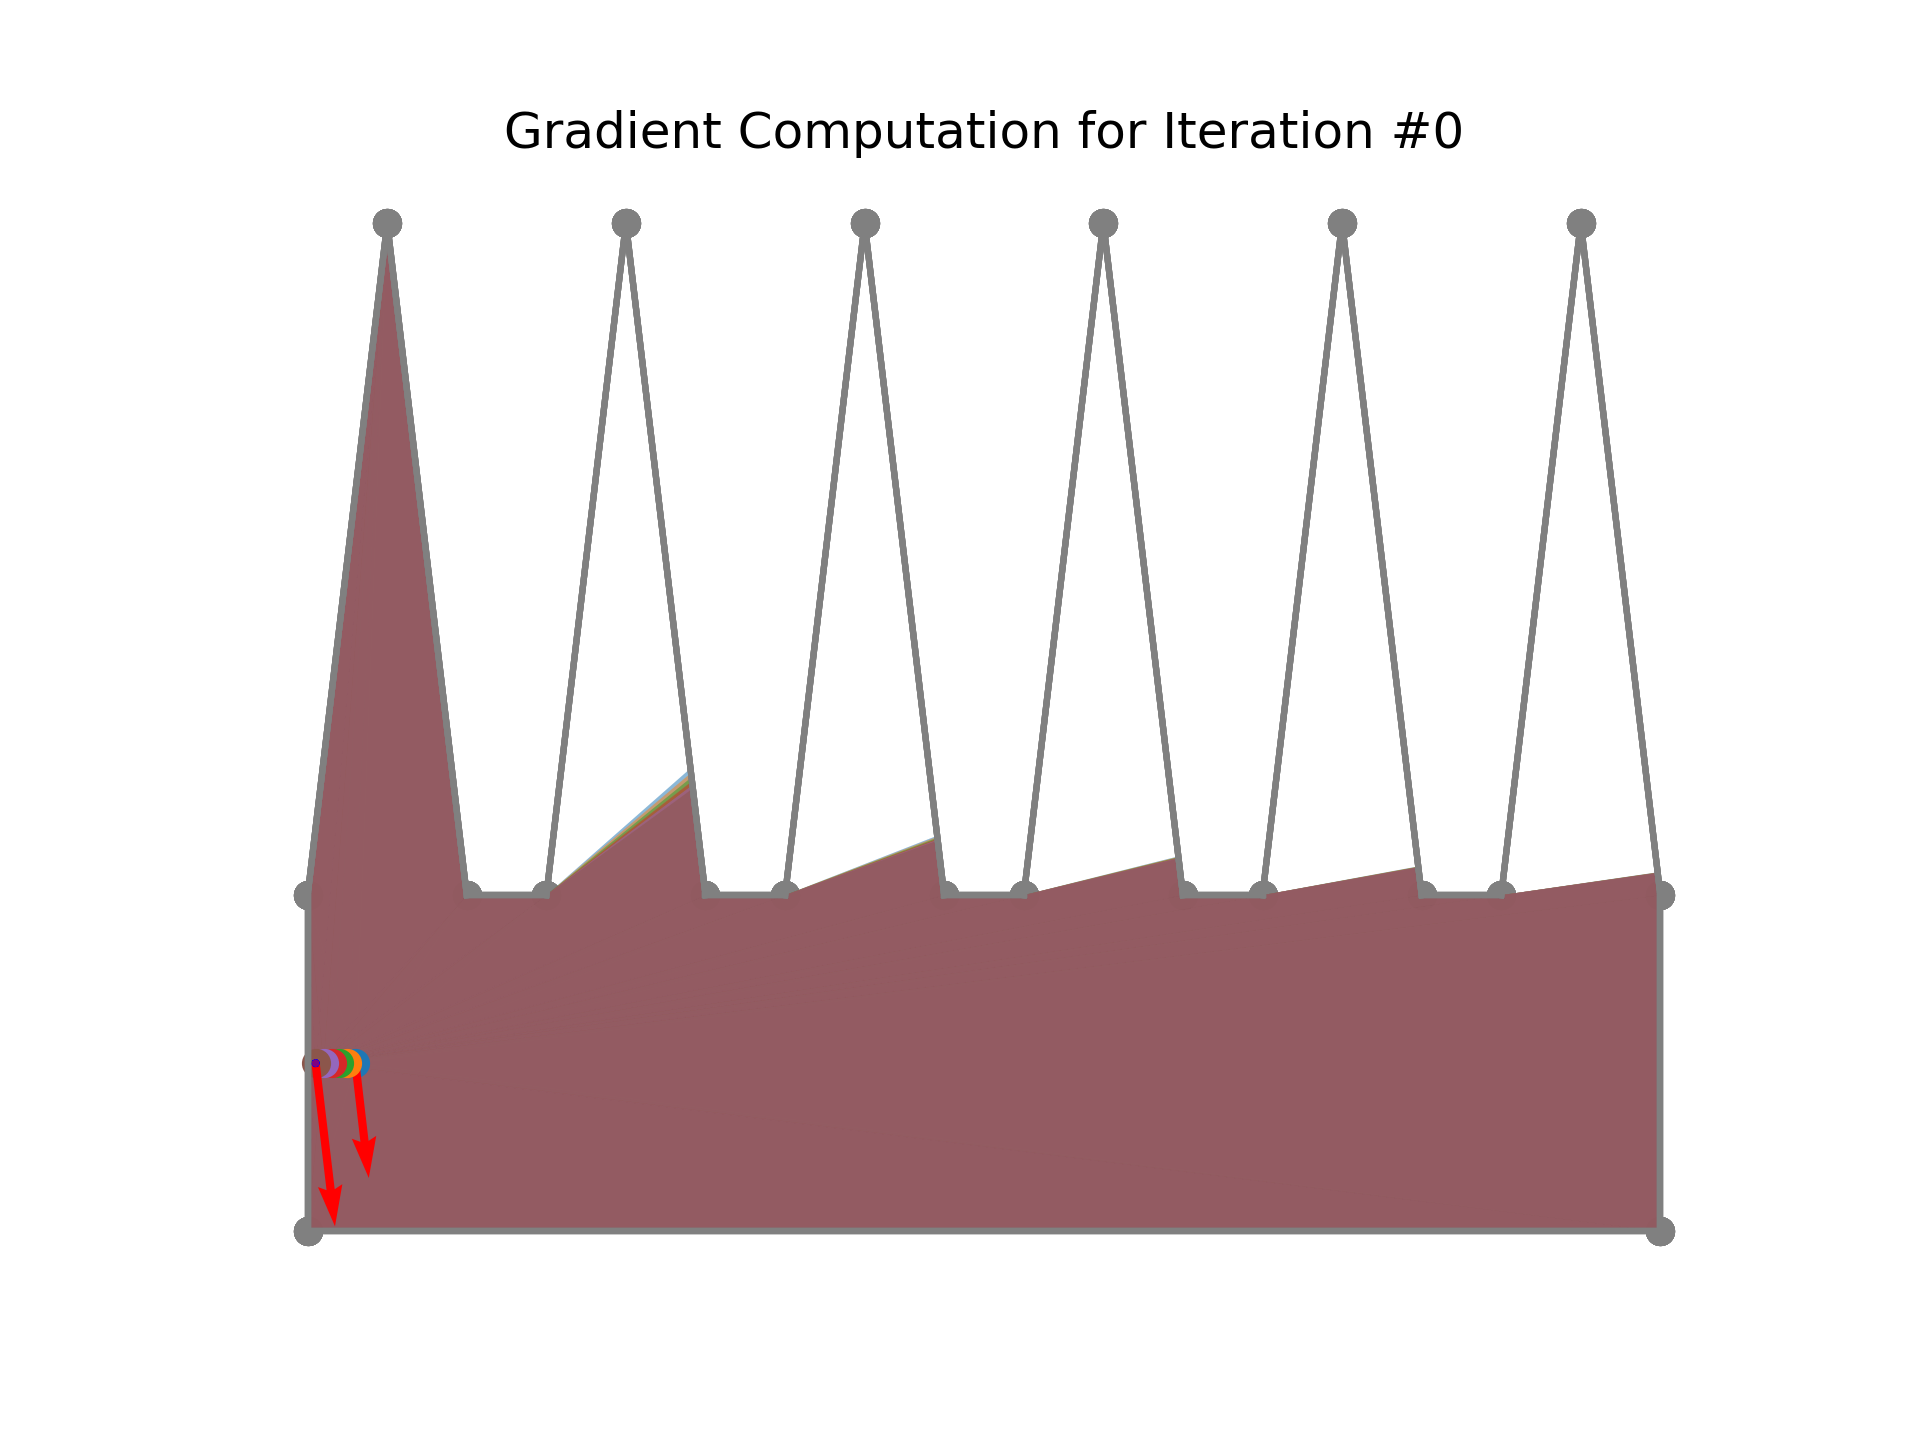
\includegraphics[width = 0.7\textwidth]{experiments/comb6_start_pos.png}
    \caption{In the comb polygon with 6 teeth, all guards start at the same $y$-coordinate, with 0.1 units in between them.}
    \label{fig:comb6_start_pos}
\end{figure}

We expect that the number of iterations and the execution time needed would scale with the number of teeth $t$ of the polygon. With every $t + 1$ tooth added, we would need the same time as before for the $t$ guards to reach their respective teeth, and some extra time for the new $t + 1^{\text{th}}$ guard. 
% We expect that the time limit would already be achieved with less than 20 comb teeth.

Figure \ref{fig:all_combs} displays the progression of our algorithm for the comb polygons with 2, 3, ..., 10, 15, 20 teeth within one hour. The comb polygons with 50 and 100 teeth did not complete any iteration within that time.
For comb polygons with 5 teeth and more than 6 teeth, the timeout was not enough to find a feasible solution. Nonetheless, it is worth discussing their behaviour, as it highlights the different issues the algorithm faces. 
For comb polygons with 7, 9 and 10 teeth, the guards appear to be stuck in a local plateau that they did not manage to escape. This is traced to an edge-case where the guards are stuck in their position because their movement vector does not improve the total area. Another reason why the guards do not move is that they are still trying to maximise their local area in the case where the total area seen cannot be increased within that step. This could result in them all moving to the same part of the polygon. Since that part of the polygon maximises their local area, they  not move anymore.
For the comb polygon with 5 teeth, the guards appear to be stuck in a local maxima that they manage to escape. Unfortunately, they later return to it and restart the cycle. It is unclear whether the comb polygon with 8 teeth would display a similar looping behaviour. Given the timeout, the guards trying to solve the comb polygon with 8 teeth display a less predictable behaviour. Hyperparameter tuning could address this issue.

\begin{figure}[h!]
    \centering
    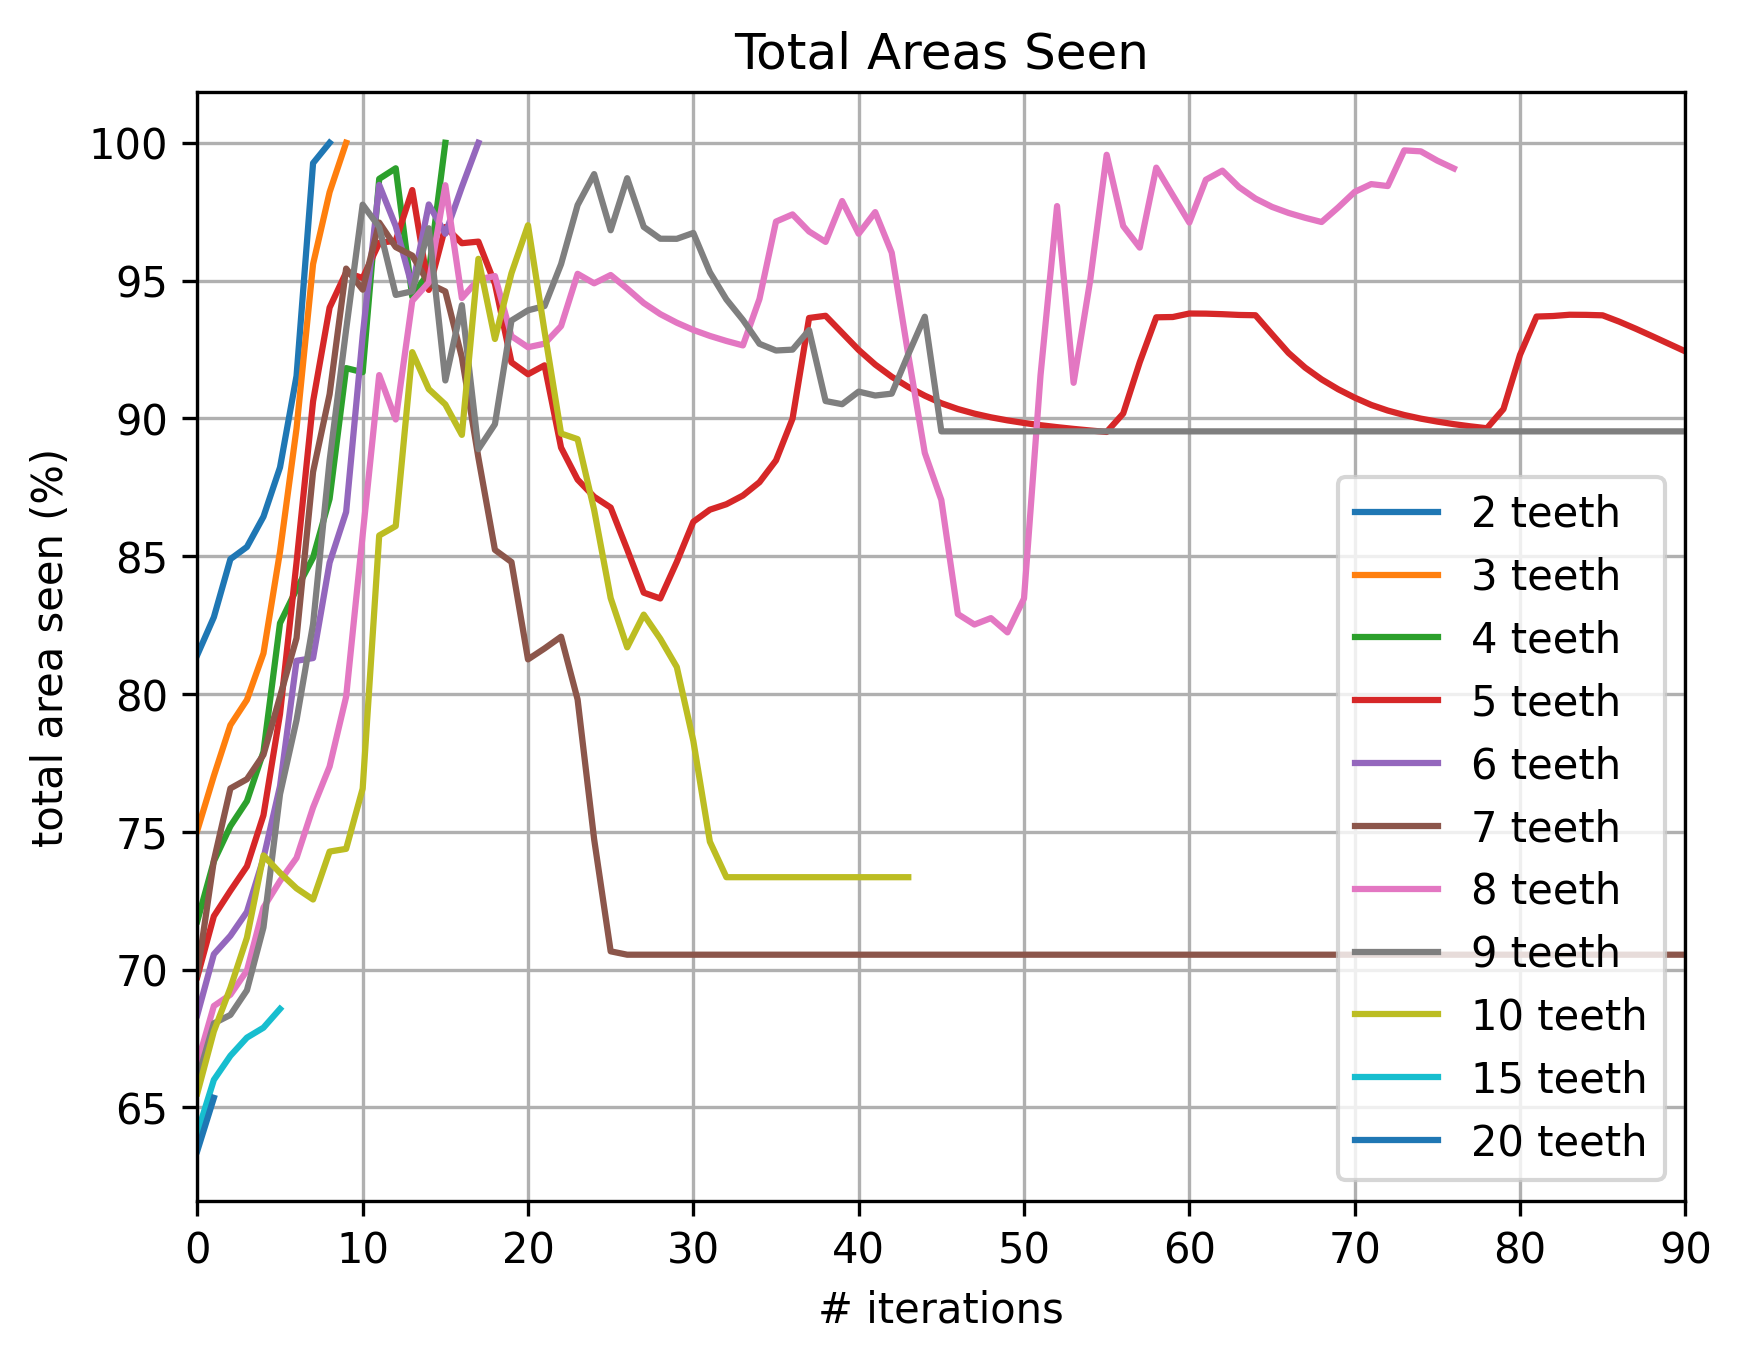
\includegraphics[width = \textwidth]{experiments/all_combs_areas.png}
    \caption{The percentage of the area seen in terms of iterations for comb polygons with 2, 3, ..., 10, 15, and 20 teeth.}
    \label{fig:all_combs}
\end{figure}

Conversely, it is also crucial to address in Figure \ref{fig:good_combs} the comb polygons which the algorithm manage to solve: 2, 3, 4 and 6 teeth. In this case, we  observe a clearer scaling: the more teeth a comb polygon has, the longer it takes to be solved. What is more, the solution also scales with the number of teeth. The comb polygon with 4 and 6 teeth take twice as many iterations to be solved than the ones with 2 and 3 teeth, respectively. We would expect a similar behaviour for comb polygons with more teeth, if the algorithms would finish.

\begin{figure}[h!]
    \centering
    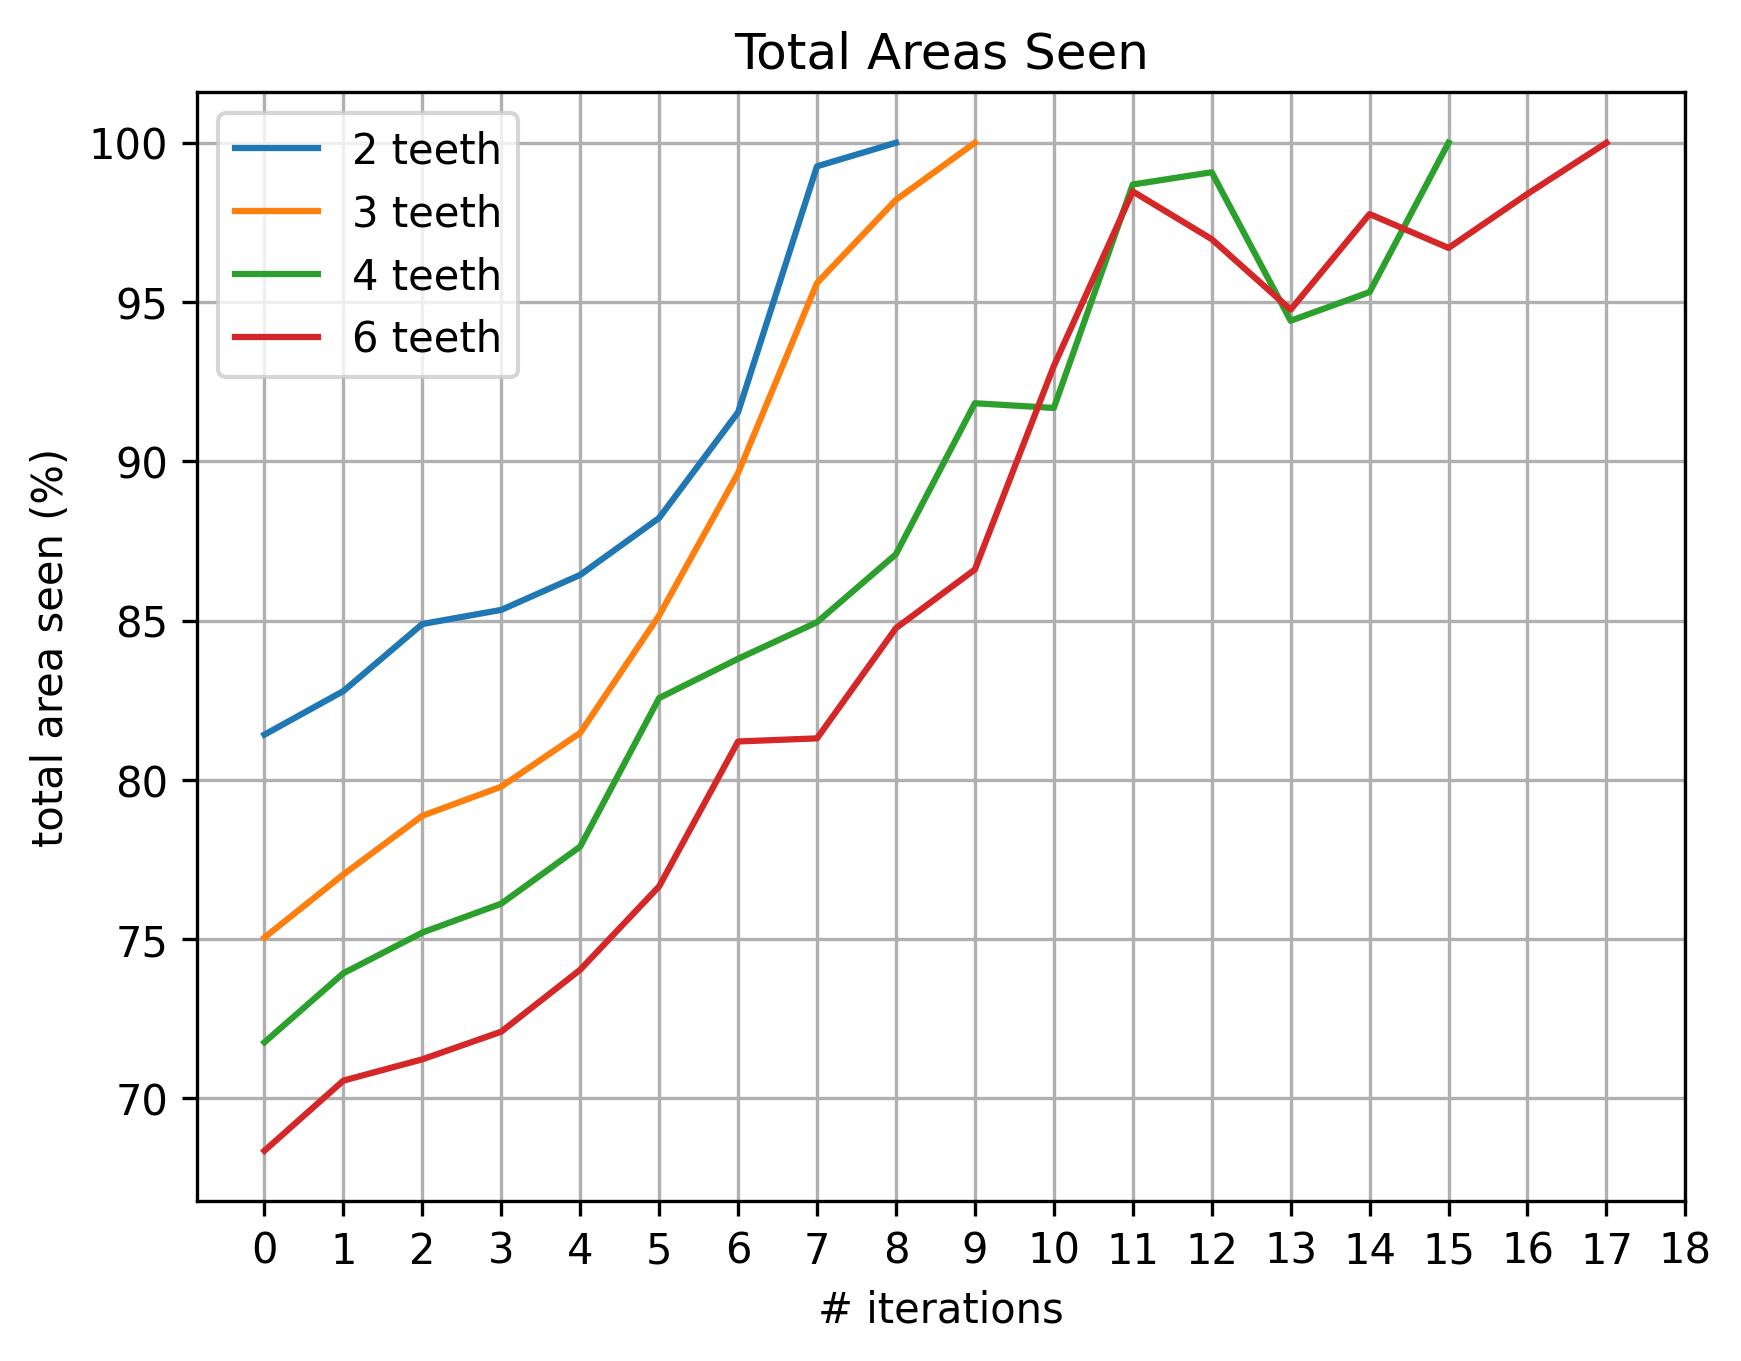
\includegraphics[width = 0.8\textwidth]{experiments/good_combs_areas.png}
    \caption{The percentage of the area seen in terms of iterations for comb polygons with 2, 3, 4, and 6 teeth.}
    \label{fig:good_combs}
\end{figure}

\newpage
It is also worth discussing how the initial guard placement and comb polygon shapes could influence the performance of the algorithm.
Firstly, it is important to note the initial placement strategy. Guards are placed in the same lower left part of the polygon. However, the larger a polygon, the lower the initially seen area. For example, we  observe how the comb polygon with 2 teeth starts at more than 80\% seen area. On the other hand, the comb polygon with 20 teeth has a less than 65\% seen area at start. We could argue that this type of placement gives larger polygons a start disadvantage. A way to mitigate this issue could be to find a way of placement that scales, while still keeping the initial similar positioning among different combs.
% \newpage

Moreover, the algorithm is sensitive to the shape of the polygons. The bigger a comb polygon grows, the sharper and narrower its teeth are. A good example in this case is Figure \ref{fig:comb20}, which displays a comb polygon with 20 teeth. Clearly, the teeth are much narrower than in the case of a comb with 4 teeth. This raises the question about the performance of the algorithm given different angles in the polygon boundary. A possible solution to this aspect would be to scale up the polygon. However, a similar question would remain: does the algorithm necessarily perform better or worse because of the polygon shape? What would be the optimal shape?

\begin{figure}[h!]
    \centering
    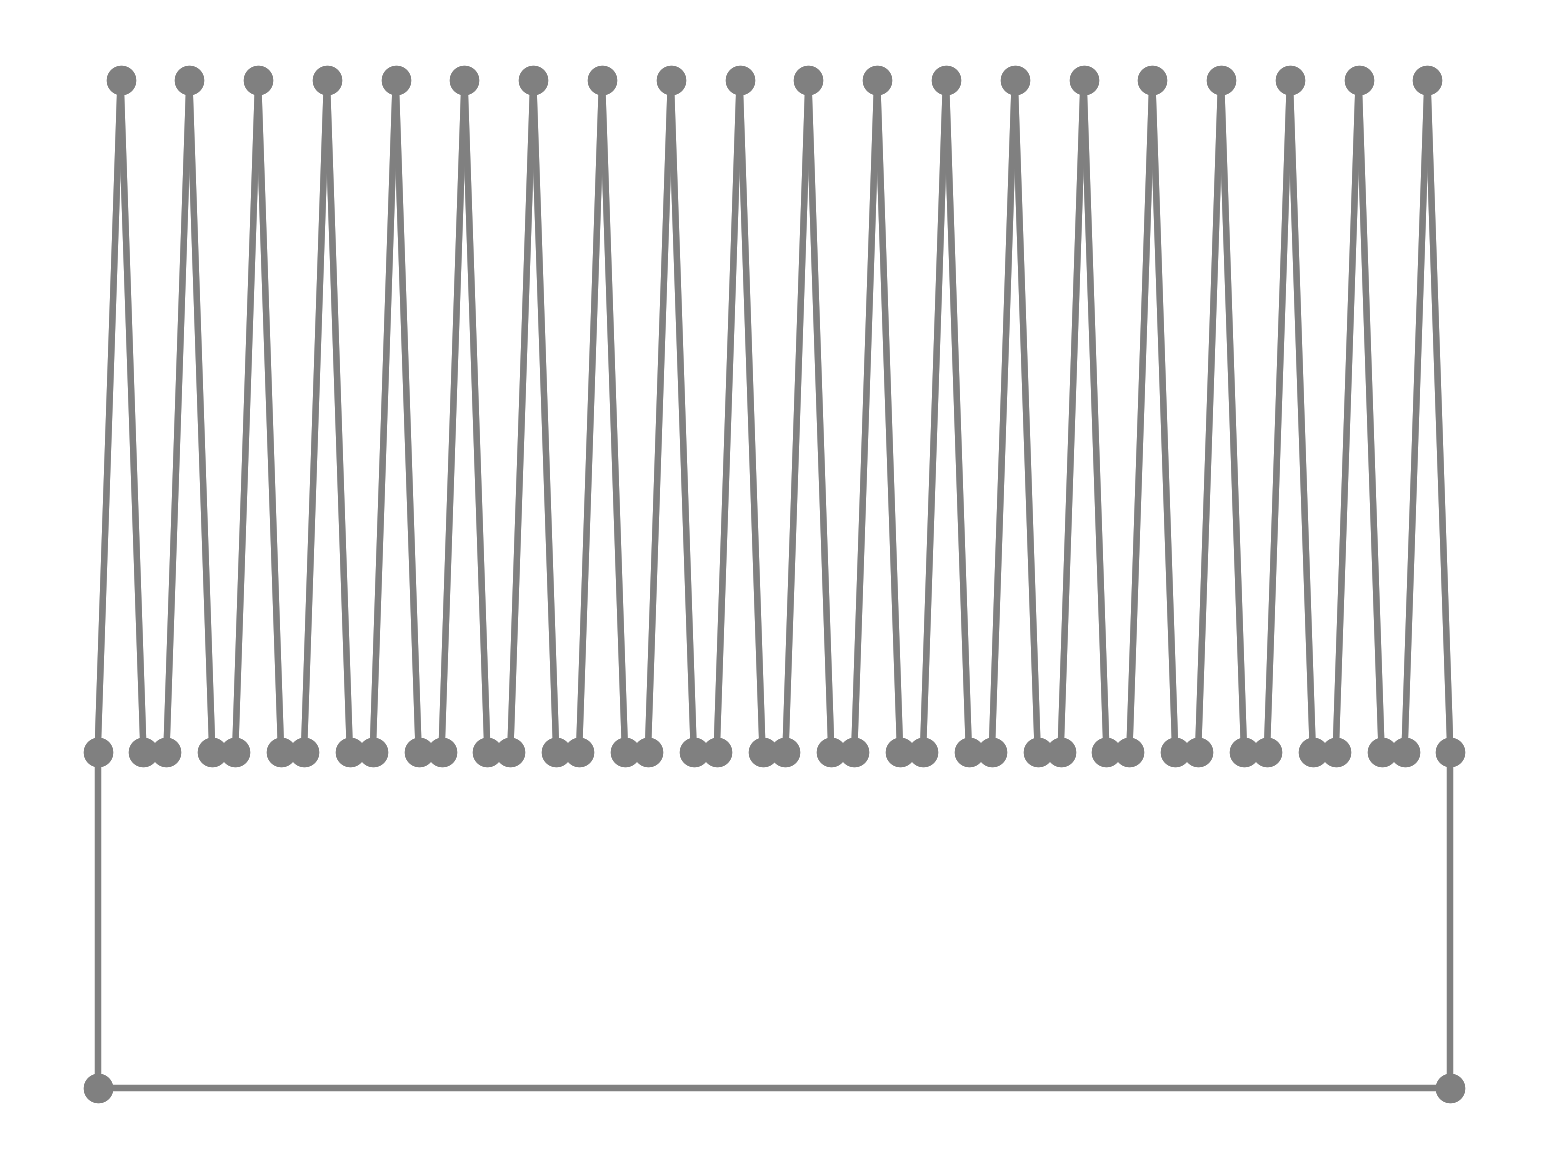
\includegraphics[width = 0.65\textwidth]{experiments/comb20.png}
    \caption{Comb polygon with 20 teeth.}
    \label{fig:comb20}
\end{figure}

\newpage
\subsection{Hyperparameter Sensitivity}
\label{sec:hyperparameters}
The algorithm is highly sensitive to the hyperparameter choices, polygon shapes and sizes, and guard starting points. We already emphasised how the hyperparameter values have been chosen: other values than the ones used would result in the program crashing or not terminating. Similarly, in the context of the comb polygon, we have discussed that the polygon shape can have a crucial effect on the performance of the algorithm.

In this section we  additionally explain how the guard starting points influence the outcome of the program. We  use the irrational guards polygon \cite{abrahamsen2021art} as an example.
The polygon can be guarded by 3 guards with irrational coordinates, or 4 guards with rational coordinates. We  thus compare these placements. We  position 3 guards at an approximation of the optimal irrational coordinates, and 4 guards at arbitrary rational coordinates. The approximated irrational guards  have coordinates $(2, 0.59), (19, 1.71), (10.57, 2.12)$. The arbitrary guards  have coordinates $(5, 0), (5.5, 0), (6, 0), (6.5, 0)$.

\begin{figure}[!h]
    \centering
    \includegraphics[width = 0.5\textwidth]{experiments/irrational_areas.png}
    \caption{Comparison for the irrational guards polygon between guards with approximately irrational coordinates and rational guard coordinates.}
    \label{fig:irrational}
\end{figure}

\newpage
Figure \ref{fig:irrational} displays the difference in runs between the previously mentioned guard placements. The orange line displays the algorithm run for the guard irrational approximation coordinates. As expected, the algorithm deems that the whole polygon is seen within the first iteration. On the other side, the blue line shows the algorithm performance for the guards with rational coordinates. Unfortunately, the program in this case crashes after the $8^{\text{th}}$ iteration. The error was unclear and the time constraints of this thesis did not allow us to solve it.

The irrational guards polygon becomes thus a suggestive example to the sensitivity of the algorithm to initial guard placements. The starting position of the guards can determine whether the algorithm is able to escape local maxima or not crash. Nonetheless, we are not able to provide a generalisation of this statement. Namely, we were not able to determine how the starting position of the guards influences the progress of the algorithm, while it is also dependent on the polygon shape.

In this way, we observed how the different heuristics influence the algorithm. Some heuristics, like momentum, proved to be fundamental to its correct development. Others, such as the pull capping, require case-specific tuning based on the start positions of the guards and the shape of the polygon.
In the next section we further discuss why the algorithm is sensitive to these hyperparameters and how it could be improved.